	%%%%%%%%%%%%%%%%%%%%%%%%%%%%%%%%%%% INICIO DE LAS CONFIGURACIONES %%%%%%%%%%%%%%%%%%%%%%%%%%%%%%%%%%%% 
\documentclass[11pt,oneside]{book}
\usepackage{geometry}								% dimensiones del documento
	\geometry{
		a4paper,									% tipo de página
		left = 25mm,								% margen izquierdo
		right = 20mm,								% margen derecho
		top = 25mm,									% margen superior
		bottom = 15mm								% margen inferior
	}
\usepackage[utf8]{inputenc}							% caracteres especiales
\usepackage[T1]{fontenc}							% permite realizar cambios al formato de separación en sílabas
\usepackage[spanish,es-tabla]{babel} 				% para ajustar algunas cuestiones como cuadro/tabla dependientes del idioma
\usepackage{enumerate}								% para ajustes de viñetas y esquemas numerados
\usepackage{helvet}									% para ajustar la tipografía a una similar a Arial
\usepackage{fancyhdr}								% para ajuste de encabezado y pie de página
\usepackage[usenames,table,xcdraw]{xcolor}			% color en documento y tablas
\usepackage{graphicx}								% para ajuste de texto en tablas
\usepackage{parskip}								% para quitar la sangría de párrafos
\usepackage{setspace}								% para ajustar el interlineado
\usepackage[autostyle]{csquotes}					% para realizar y mostrar citas 'inline'
\usepackage{amsmath}								% para poder utilizar ecuaciones en diferentes entornos, por ejemplo, listas numeradas y viñetas
\usepackage[T1,hyphens]{url}						% para separar en más de una línea URLs muy largas
\usepackage[colorlinks=true,
            linkcolor=bunl,
            urlcolor=bunl,
            citecolor=bunl]{hyperref}				% para links en color
\usepackage{titlesec}								% para formatear secciones, subsecciones, etc.
\usepackage{enumitem}								% para modificar la identación de listas numeradas
\usepackage{tocloft}								% para ajustar la posición en la página de la tabla de contenidos	
\usepackage{pdflscape}
\usepackage{multicol}

\usepackage{listings}								% para agregar código de programación al documento
% ******* PARÁMETROS DE CONFIGURACIÓN PARA ALGORITMOS ******
\definecolor{mygreen}{rgb}{0,0.6,0}
\definecolor{mygray}{rgb}{0.5,0.5,0.5}
\definecolor{mymauve}{rgb}{0.58,0,0.82}
\lstset{ 
	language=php,	
	breaklines=true,	
	frame=none,
	escapeinside={\%*}{*){Ó}},
	basicstyle=\footnotesize,
	keywordstyle=\textcolor{blue},
	numberstyle=\color{mygray},
	commentstyle=\color{mygreen},
	numbers=left,
	numbersep=4pt,
	stringstyle=\color{mymauve},
	showstringspaces=false,
	inputencoding=utf8
	%    backgroundcolor=\color{gray!10},
%    frame=single,
%    tabsize=2,
%    rulecolor=\color{black!30},
%    title=\lstname,
%    escapeinside={\%*}{*)},
%
%    breakatwhitespace=true,
%    framextopmargin=2pt,
%    framexbottommargin=2pt,
%    extendedchars=false,
%    inputencoding=utf8
}

% ******* FIN DE CONFIGURACIÓN DE ALGORITMOS ******
%\usepackage[spanish]{algorithm2e}

\hyphenation{bie-nes-tar}							%ajuste de palabras en silabas

% ajuste de la tipografía a una similar a Arial
\renewcommand{\familydefault}{\sfdefault}

% Para que no aparezca la numeración del capítulo en el número de la subsección
\renewcommand*\thesection{\arabic{section}}

% ajuste de la profundidad para numeración de secciones, subsecciones, etc.
\setcounter{secnumdepth}{4}		% en el documento
\setcounter{tocdepth}{3}		% en la tabla de contenidos

% formato de secciones
\titleformat{\section}{\normalfont\fontsize{12}{14}\bfseries}{\thesection.}{1 em}{}
\titlespacing*{\section}{0pt}{6mm}{4mm}

% formato de subsecciones
\titleformat{\subsection}{\normalfont\fontsize{12}{14}\bfseries}{\thesubsection.}{1 em}{}
\titlespacing*{\subsection}{0pt}{2mm}{1mm}

% formato de subsubsecciones
\titleformat{\subsubsection}{\normalfont\fontsize{11}{13}\bfseries}{\thesubsubsection.}{1 em}{}
%\titlespacing*{\subsection}{0pt}{-1mm}{-1mm}

% ajuste de encabezado y pie de página
\pagestyle{fancy}									% activa el estilo de encabezado y pie de página
\fancyhead{}										% borra el formato del encabezado
\renewcommand{\headrulewidth}{0pt}					% quita la barra horizontal del encabezado
\fancyfoot{}										% borra el formato del pie de página
\fancyfoot[R]{\fontsize{8}{10}\thepage}				% numeración en el borde inferior derecho

% definición de colores personalizados
\definecolor{b}{rgb}{0.3,0.3,1}						% color azul definido por mí (no es azul puro...tiene un toque de rojo y verde)
\definecolor{bunl}{rgb}{0,0.4941,0.6392}			% color azul institucional de UNL
\definecolor{w}{rgb}{1,1,1}							% color blanco
\definecolor{k}{rgb}{0,0,0}							% color negro
\definecolor{r}{rgb}{1,0,0}							% color rojo
\definecolor{g}{rgb}{0.3,1,0.3}						% color verde definido por mí (no es verde puro...tiene un toque de rojo y azul)

% para texto en monospace color azul
\newcommand\ff[1]{{\scshape\color{bunl}#1}}

% para cambiar a tipo de letra bash o shell
\newcommand*{\mf}{\fontfamily{cmtt}\selectfont}

% defaults para niveles de viñetas
\renewcommand\labelitemi{$\bullet$}	% 1er. nivel - diamante (diamond)
\renewcommand\labelitemii{$\bullet$}		% 2do. nivel - círculo relleno (bullet)
\renewcommand\labelitemiii{$\circ$}		% 3er. nivel - círculo (circle)
\renewcommand\labelitemiv{$-$}			% 4to. nivel - guión (símbolo menos)

% separación entre items
\setlist[1]{itemsep=-4 pt}
\setlist[2]{itemsep=-8 pt}
\setlist[3]{itemsep=-12 pt}

% Para evitar los warnings por overfull y underfull hbox y vbox
\hfuzz=20pt
\vfuzz=20pt
\hbadness=10000
\vbadness=\maxdimen

% para corregir la separación en sílabas de algunas palabras en particular
\hyphenation{mé-to-dos}

%Cosas para Rieso
\usepackage{tcolorbox}
\newtcolorbox{mybox}{colback=color_riesgo,colframe=colriesgo,arc=0mm,boxrule=0.2mm}
\definecolor{color_riesgo}{RGB}{154,175,194} %fondo
\definecolor{colriesgo}{RGB}{26,51,0} %Recuadro y letra del nombre

\usepackage{multirow, array}

\usepackage{etoolbox}

\makeatletter
\patchcmd{\ttlh@hang}{\parindent\z@}{\parindent\z@\leavevmode}{}{}
\patchcmd{\ttlh@hang}{\noindent}{}{}{}
\makeatother

%%%%%%%%%%%%%%%%%%%%%%%%%%%%%%%%%%%%% FIN DE LAS CONFIGURACIONES %%%%%%%%%%%%%%%%%%%%%%%%%%%%%%%%%%%%% 

%%%%%%%%%%%%%%%%%%%%%%%%%%%%%%%%%%%%%%%%% TÍTULO Y ENCABEZADO %%%%%%%%%%%%%%%%%%%%%%%%%%%%%%%%%%%%%%%%
\begin{document}
% ajuste del interlineado a 2 líneas para el título
\doublespacing
\begin{center}
\LARGE Diseño y Desarrollo de un Software de Gestión y Seguimiento de Trazabilidad de Ganado Vacuno
\end{center}

\vspace{0.25cm}
\begin{center}
\rule{\textwidth}{.4pt}
\end{center}
\vspace{0.25cm}

% ajuste del interlineado a 0.95 líneas para la sección de autor
\spacing{0.95}

\textbf{Autor:} Mario A. Rosales (mariorosales941@gmail.com)

\textbf{Director:} Ing. Lucila Romero (lucila.rb@gmail.com)

%\textbf{Co-Director:} 

\textbf{Asesor Temático:}
\begin{itemize}
\item Ing. Agrónomo Jorge Cinquini
\item Med. Veterinario Juan Carlos Garcia
\end{itemize}

\begin{center}
\rule{\textwidth}{.4pt}
\end{center}
\vspace{3.5mm}

\begin{center}
\textbf{\Large Informe Final}
\end{center}

\begin{center}
\rule{\textwidth}{.4pt}
\end{center}
% ajuste del interlineado para el resto del documento
\spacing{1.15}

% ajuste de la separación entre párrafos
\setlength{\parskip}{5mm}

%%%%%%%%%%%%%%%%%%%%%%%%%%%%%%%%%%%%%% RESUMEN Y PALABRAS CLAVE %%%%%%%%%%%%%%%%%%%%%%%%%%%%%%%%%%%%%%

%%%%%%%%%%%%%%%%%%%%%%%%%%%%%%%%%%%%%%%%% TABLA DE CONTENIDOS %%%%%%%%%%%%%%%%%%%%%%%%%%%%%%%%%%%%%%%%
\clearpage
\newpage
% quita el espacio antes del margen superior en la tabla de contenidos
\setlength{\cftbeforetoctitleskip}{0pt}			

% para ajustar la fuente del título de la tabla de contenidos
\renewcommand{\cfttoctitlefont}{\Large\bfseries}	
\tableofcontents

\clearpage
\newpage

%%%%%%%%%%%%%%%%%%%%%%%%%%%%%%%%%%%%%%%% INICIO DEL DOCUMENTO %%%%%%%%%%%%%%%%%%%%%%%%%%%%%%%%%%%%%%%%
\chapter{Análisis de Requerimientos}
\section{Etapa 1 - Análisis de Requerimientos 2}

\subsection{Ingeniería de Requerimientos}
\subsubsection{Introducción}
En \textit{Ingeniería de Software}, la \textit{Ingeniería de Requerimientos} comprende todas las tareas relacionadas con la determinación de las necesidades o las condiciones que un software debe satisfacer, tomando en cuenta los diversos requisitos de las partes interesadas. El propósito esta disciplina es hacer que los mismos alcancen un estado óptimo antes de alcanzar la fase de diseño, en todo proyecto.

La \textit{Ingeniería de Requerimientos} cumple un papel primordial en el proceso de producción de software, ya que enfoca un área fundamental: la definición de lo que se desea producir. Su principal tarea consiste en la generación de especificaciones correctas que describan con claridad, sin ambigüedades, en forma consistente y compacta, el comportamiento del sistema; de esta manera, se pretende minimizar los problemas relacionados al desarrollo de sistemas.

Si bien existen muchas definiciones para requerimiento, ha continuación se presenta la definición que aparece en el glosario de la \textit{IEEE}:

\begin{itemize}
\item \textit{Una condición o necesidad de un usuario para resolver un problema o alcanzar un objetivo.}
\item \textit{Una condición o capacidad que debe estar presente en un sistema o componentes de sistema para satisfacer un contrato, estándar, especificación u otro documento formal.}
\item \textit{Una representación documentada de una condición o capacidad, como en los casos anteriores.}
\end{itemize}

Sommerville (2005) afirma que cuando hablamos de requerimientos debemos saber que existen requerimientos funcionales y no funcionales.
\begin{itemize}
\item \textbf{\textit{Requerimientos Funcionales}}: \textit{son declaraciones de los servicios que debe proporcionar el sistema, de la manera en que éste debe reaccionar ante entradas particulares y de cómo se debe comportar en diversas situaciones.} 

%\textit{Los requerimientos funcionales definen las funciones que el sistema será capaz de realizar. Describen las transformaciones que el sistema realiza sobre las entradas para producir salidas.}

\item \textbf{\textit{Requerimientos No Funcionales}}: \textit{son restricciones de los servicios o funciones ofrecidos por el sistema. Incluyen las restricciones de tiempo, sobre el proceso de desarrollo y estándares.}

%\textit{Los requerimientos no funcionales tienen que ver con características que de una u otra forma puedan limitar el sistema, como por ejemplo, el rendimiento (en tiempo y espacio), interfaces de usuario, fiabilidad (robustez del sistema, disponibilidad de equipo), mantenimiento, seguridad, portabilidad, estándares, etc.}
\end{itemize}

\newpage
Las características de un requerimiento son sus propiedades principales. Un conjunto de requerimientos en estado de madurez, debe presentar una serie de características tanto individualmente como en grupo. A continuación se presentan las propiedades de los requerimientos, según la IEEE:
\begin{itemize}
\item \textit{\textbf{Necesario}}: \textit{un requerimiento es necesario si su omisión provoca una deficiencia en el sistema a construir, y además su capacidad, características físicas o factor de calidad no pueden ser reemplazados por otras capacidades del producto o del proceso.}

\item \textit{\textbf{Conciso}}: \textit{un requerimiento es conciso si es fácil de leer y entender. Su redacción debe ser simple y clara para aquellos que vayan a consultarlo en un futuro.}

\item \textit{\textbf{Completo}}: \textit{un requerimiento está completo si no necesita ampliar detalles en su redacción, es decir, si se proporciona la información suficiente para su comprensión.}

\item \textit{\textbf{Consistente}}: \textit{un requerimiento es consistente si no es contradictorio con otro requerimiento.}

\item \textit{\textbf{No ambiguo}}: \textit{un requerimiento no es ambiguo cuando tiene una sola interpretación. El lenguaje usado en su definición, no debe causar confusiones al lector.}

\item \textit{\textbf{Verificable}}: \textit{un requerimiento es verificable cuando puede ser cuantificado de manera que permita hacer uso de los siguientes métodos de verificación: inspección, análisis, demostración o pruebas.}
\end{itemize}

A continuación se darán algunas definiciones para ingeniería de requerimientos:
\begin{itemize}
\item \textit{Ingeniería de Requerimientos ayuda a los ingenieros de software a entender mejor el problema en cuya solución trabajarán. Incluye el conjunto de tareas que conducen a comprender cuál será el impacto del software sobre el negocio, qué es lo que el cliente quiere y cómo interactuarán los usuarios finales con el software.} (Pressman, 2006: 155).

\item \textit{Ingeniería de Requerimientos es el proceso de desarrollar una especificación de software. Las especificaciones pretender comunicar las necesidades del sistema del cliente a los desarrolladores del sistema.} (Sommerville, 2005: 82) 

\item \textit{Ingeniería de Requerimientos es la disciplina para desarrollar una especificación completa, consistente y no ambigua, la cual servirá como base para acuerdos comunes entre todas las partes involucradas y en dónde se describen las funciones que realizará el sistema.} (Boehm 1979).

\item \textit{Es el proceso mediante el cual se intercambian diferentes puntos de vista para recopilar y modelar lo que el sistema va a realizar. Este proceso utiliza una combinación de métodos, herramientas y actores, cuyo producto es un modelo del cual se genera un documento de requerimientos.} (Leite 1987).
\end{itemize}

\subsubsection{Actividades de la Ingeniería de Requerimientos}
Cinco actividades básicas se deben llevar a cabo para completar el proceso de recolección de requerimientos. Realizar las mismas ayudan a reconocer la importancia que tiene para el desarrollo de un proyecto de software realizar una especificación y administración adecuada de los requerimientos de los clientes o usuarios. Las actividades son:
\begin{itemize}
\item \textit{\textbf{Obtener requisitos}: es como comúnmente se denomina a las actividades involucradas en el descubrimiento de los requerimientos del sistema.}
%Aquí, los analistas de requerimientos deben trabajar junto al cliente para descubrir el problema que el sistema debe resolver, los diferentes servicios que el sistema debe prestar y las restricciones que se pueden presentar.

\item \textit{\textbf{Analizar requisitos}: se enfoca en descubrir problemas con los requerimientos del sistema identificados hasta el momento.}
%Detectar y corregir las falencias comunicativas, transformando los requerimientos  obtenidos en condiciones apropiadas para ser tratados en el diseño.

\item \textit{\textbf{Documentar requisitos}: en esta fase se documentan los requerimientos acordados con el cliente, en un nivel apropiado de detalle.}
%se puede decir que al documentar se está haciendo una descripción detallada del análisis realizado previamente, aplicando técnicas y/o estándares de documentación, como la notación UML (Lenguaje de Modelado Unificado), que es un estándar para el modelado orientado a objetos.

\item \textit{\textbf{Verificar los requisitos}: consiste en comprobar el correcto funcionamiento de un requisito en la aplicación.}

\item \textit{\textbf{Validar los requisitos}: en esta fase, el objetivo es ratificar los requerimientos, es decir, verificar todos los requerimientos que aparecen en el documento especificado para asegurarse que representan una descripción, por lo menos, aceptable del sistema que se debe implementar.}
%Esto implica verificar que los requerimientos sean consistentes y que estén completos.
\end{itemize}

\subsubsection{Interesados o Stakeholders}
Se identificaron a todas aquellas personas o grupo de ellas que se verán afectados por el sistema, ya sea de forma directa o indirecta; Sommerville (2005) denomina a éstos como \textit{stakeholders}. Los stakeholders identificados son: 
\begin{itemize}
\item \textit{\textbf{Alumno}}: \textit{autor del presente proyecto.}
\item \textit{\textbf{Director}}: \textit{quien se encarga de coordinar y gestionar, como así también de guiar al alumno a lo largo de todo el desarrollo del proyecto.}
\item \textit{\textbf{Asesores Temáticos}}: \textit{quienes prestan colaboración para con el alumno, brindando información y compartiendo conocimiento basado en su formación y experiencia.}
\item \textit{\textbf{Docentes}}: \textit{quienes forman el cuerpo docente de la Cátedra de Proyecto Final de Carrera.}
\item \textit{\textbf{Usuarios}}: \textit{quienes van a utilizar el software, pudiendo ser dueños o empleados de la empresa o entidad ganadera.}
\end{itemize}

\newpage
\subsubsection{Ingeniería de Requerimientos: Técnicas y Herramientas}
Serán mencionadas algunas de las técnicas mas populares. En la práctica, la técnica más apropiada para cada actividad dependerá del proyecto que se esté desarrollando.
\begin{itemize}
\item \textit{\textbf{Entrevistas}: la entrevista es de gran utilidad para obtener información cualitativa como opiniones, o descripciones subjetivas de actividades.} 
%Es una técnica muy utilizada, y requiere una mayor preparación y experiencia por parte del analista. La entrevista se puede definir como un ``intento sistemático de recoger información de otra persona'' a través de una comunicación interpersonal que se lleva a cabo por medio de una conversación estructurada. Es muy importante la forma en que se plantea la conversación y la relación que se establece en la entrevista.

\item \textit{\textbf{Observación}: por medio de esta técnica el analista obtiene información de primera mano sobre la forma en que se efectúan las actividades.}
%Este método permite observar la forma en que se llevan a cabo los procesos y, por otro, verificar que realmente se sigan todos los pasos especificados. Como sabemos, en muchos casos los procesos son una cosa en papel y otra muy diferente en la práctica. Los observadores experimentados saben qué buscar y cómo evaluar la relevancia de lo que observan.

\item \textit{\textbf{Estudio de documentación}: varios tipos de documentación, como manuales y reportes, pueden proporcionar al analista información valiosa con respecto a las organizaciones y a sus operaciones.} 
%La documentación difícilmente refleja la forma en que realmente se desarrollan las actividades, o donde se encuentra el poder de la toma de decisiones. Sin embargo, puede ser de gran impotancia para introducir al analista al dominio de operación y el vocabulario que utiliza.

\item \textit{\textbf{Tormenta de Ideas (Brainstorming)}: consiste en reuniones con pocas personas donde como primer paso sugieren toda clase de ideas sin juzgar su validez, y luego se realiza un análisis detallado de cada propuesta.} 
%Esta técnica se puede utilizar para identificar un primer conjunto de requisitos en aquellos casos donde no están muy claras las necesidades que hay que cubrir, o cuando se esta creando un sistema que habilitará un servicio nuevo para la organización.
\end{itemize}

La Entrevista y la Observación fueron claves para recolectar los requerimientos de este trabajo. Esto se debe, principalmente, a la naturaleza del mismo. Las siguientes, son algunas de las preguntas que se formularon y realizaron a los \textit{asesores temáticos}:
\begin{itemize}
\item \textit{¿Cuáles son las Razas Vacunas que existen en Argentina?}
\item \textit{¿Cuáles son sus características, qué producto se obtiene, fortalezas, debilidades, ventajas y desventajas de trabajar con estas Razas?}
\item \textit{¿Cómo es el ciclo de vida de un vacuno?}
\item \textit{¿Cuál es el clima adecuado para trabajar con cada Raza y con qué características debe contar el lugar en donde se alojan los animales?}
\item \textit{¿Cómo debe ser su alimentación?}
\item \textit{¿Cuáles son los aspectos mas importantes a tener en cuenta en este tipo de negocio?}
\item \textit{¿Cuáles son los cuidados sanitarios que deben tenerse o respetarse para con los vacunos?}
\item \textit{¿Cuáles fueron las razones por las que se ha decido utilizar un sistema informático como herramienta para facilitar las labores?}
\item \textit{¿De qué manera el nuevo software los beneficiará o ayudará?}  
\item \textit{¿El nuevo software, qué esperan que haga por ustedes?}
\end{itemize}

\newpage
Luego de haber confeccionado las preguntas, se coordino con las personas a entrevistar un lugar, día y horario para realizar las entrevistas. Los asesores son:
\begin{itemize}
\item \textbf{Ing. Agro. Jorge Cinquini}: dueño y gerente general de la empresa ganadera que se tomó como caso de estudio y sobre la cual se basó el proyecto. La empresa tiene cerca de $10$ años de trayectoria en la cría y producción de ganado y cuenta con mas de $2500$ cabezas. Como profesional, dedica su vida a llevar adelante la empresa tomando las decisiones necesarias para lograr el bienestar tanto de empleados como de animales. 

La empresa cuenta con $3$ campos en los cuales se encuentran distribuidos los bovinos. Esta distribución no es equitativa y encuentra sus fundamentos a raíz de diversas razones, ejemplo de estas suelen ser razones climáticas o estratégicas. Por ejemplo, puede ocurrir que debido a inundaciones sea necesario trasladar vacunos de un campo a otro ó, buscando alimentar con mejores pasturas a aquellos vacunos que hayan sido destinados para engorde y, posteriormente, vendidos a frigoríficos.

\item \textbf{Med. Vet. Juan Carlos Garcia}: es el médico veterinario encargado de los campos que posee la empresa. Cuenta con la colaboración de colegas, los cuales también formaron parte de las entrevistas, para controlar y realizar actividades sanitarias como así también de identificación y distribución de bovinos, siendo estas últimas las principales disparadores de elaborar un sistema preciso para lograr el seguimiento.
\end{itemize} 

Las entrevistas realizadas revelaron la mayoría de los requerimientos encontrados. Mientras que, las observaciones de actividades de campo, permitieron encontrar nuevos requerimientos, como así también aclarar y refinar los ya encontrados.

\subsection{Requerimientos Identificados}
De esta manera, siguiendo con las técnicas de recopilación de requerimientos mencionadas anteriormente, se obtuvieron los requerimientos funcionales y no funcionales que definen las características con las que deberá contar el software a ser desarrollado. A continuación, se procede a listar los requerimientos obtenidos junto con la descripción de cada uno de ellos, buscando expresar, de manera breve, la importancia de los mismos en dicho trabajo. 

\subsubsection{Requerimientos Funcionales.}
Los requerimientos funcionales que se han encontrado, son los siguientes:
\begin{itemize}

\item \textit{\textbf{RF01 - Registro y Autenticación de Usuarios}}: \textit{el sistema debe permitir el registro y autenticación de usuarios.}

\item \textit{\textbf{RF02 - Perfiles de Usuario}}: \textit{el sistema debe contar con varios perfiles que permitan acceder a distintas características o funcionalidades. Los perfiles con los que contará el software son: perfil Administrador, perfil Veterinario y un perfil Peón.}

\item \textit{\textbf{RF03 - RBAC (Control de Acceso Basado en Roles)}}: \textit{el sistema debe ser capaz de implementar este tipo de control, para salvaguardar la información.}

\item \textit{\textbf{RF04 - Validación}}: \textit{el sistema debe validar que la información ingresada por el usuario sea correcta, respetando los tipos y formatos predefinidos.}

\item \textit{\textbf{RF05 - Carga de Información de Campos}: el sistema debe contar con un modulo para configuración de Campos, en los cuales, se tengan animales. Junto con ello, deberá permitir que el usuario defina la manera en que los vacunos serán dispuestos, es decir, geográficamente, en dicho campo. En otras palabras, el sistema debe permitir al usuario dividir sus tierras por lotes, por potreros, por zonas, por corrales, entre otros.}

\item \textit{\textbf{RF06 - Carga de Información de Razas}}: \textit{el sistema debe contar con un módulo para configuración de Razas con las que se desee trabajar. A través de dicho módulo, la empresa pueda ajustar el sistema a sus necesidades, es decir, con qué de razas, categorías y subcategorías llevan adelante sus actividades.}

\item \textit{\textbf{RF07 - Registro de Vacunos}}: \textit{el sistema, a la hora de ingresar un nuevo vacuno, debe permitir asignarle un identificador, como así también ingresar información adicional sobre el bovino como por ejemplo raza, línea genética, premios obtenidos, progenitores, peso, condición corporal, categoría, edad, entre otros.}

\item \textit{\textbf{RF08 - Carga de Información de Vacunos}}: \textit{el sistema debe permitir la carga de las las actividades sanitarias, reproductivas y alimenticias realizadas sobre los bovinos, como vacunaciones, modificaciones en la dieta según la edad, servicios, entre otras.}

\item \textit{\textbf{RF09 - Stock}}: \textit{el sistema debe permitir visualizar en tiempo real el stock de animales. El mismo debe estar presentado de manera clara, discriminando por razas, categorías y subcategorías.}

\item \textit{\textbf{RF10 - Registro de Operaciones}}: \textit{El sistema debe contar con un módulo para el registro de operaciones. Entre ellas, se encuentran la Compra, Venta, Cambio de Categoría, Mortandad, entre otras, referentes al ciclo de vida de la empresa y los animales.}

\item \textit{\textbf{RF11 - Creación de Eventos}}: \textit{el sistema debe permitir la creación de eventos que permitan llevar adelante el seguimiento de los vacunos. Un ejemplo de estos eventos suelen ser, por ejemplo, cuándo dar servicio a las hembras y cuándo realizar tacto sobre las mismas.}

\item \textit{\textbf{RF12 - Notificaciones}}: \textit{el sistema debe notificar al usuario ante el advenimiento de algún evento. El aviso se hará a través del envió de un correo electrónico a los usuarios interesados y, a través de mensajes en ventanas popup dentro del sistema.}

\item \textit{\textbf{RF13 - Creacion de Reportes}}: \textit{el sistema debe permitir la creación de reportes mediante los cuales se pueda obtener, de manera resumida, la información almacenada en el sistema. Entre los reportes mas comunes se encuentran el resumen de stock, el resumen de operaciones realizas en un período específico o la información de un vacuno en particular.}

\item \textit{\textbf{RF14 - Log}}: \textit{el sistema debe poder llevar algún tipo de registro de accesos al sistema, de operaciones o consultas realizadas. En caso de ocurrir algún error, esto será de utilidad para poder identificar el motivo que dió origen al mismo.}
\end{itemize}

\subsubsection{Requerimientos No Funcionales}
\begin{itemize}

\item \textit{\textbf{RNF01 - Disponibilidad (Availability)}}: \textit{medida de disponibilidad del sistema para su uso. El sistema debe estar disponible para su uso las 24 hr del día.} %(Barbacci et al.,1995)

\item \textit{\textbf{RNF02 - Seguridad/Confidencialidad (Confidentiality)}}: \textit{ausencia de acceso no autorizado a la información. El sistema debe brindar un servicio de control de acceso basado en roles, con el mismo se espera brindar protección a los datos e información tanto de usuarios como propias del negocio. La aplicación estará habilitada solo para aquellos usuarios registrados. Se deberá validar la autenticación de usuario al momento de interactuar con el sistema.} %(Barbacci et al., 1995)

\item \textit{\textbf{RNF03 - Funcionalidad (Functionality)}}: \textit{habilidad del sistema para realizar el trabajo para el cual fue concebido. El sistema debe comportarse de manera adecuada, según los objetivos para los cuales se lo haya creado.} %(Kazman et al., 2001)

\item \textit{\textbf{RNF04 - Desempeño (Performance)}}: \textit{grado en el cual un sistema o componente cumple con sus funciones designadas, dentro de ciertas restricciones dadas, como velocidad, exactitud o uso de memoria. Los tiempos de respuesta que serán tolerados deberán estar por debajo de 5 segundos.} %(IEEE 610. 12)

\item \textit{\textbf{RNF05 - Confiabilidad (Reliability)}}: \textit{medida de la habilidad de un sistema de mantenerse operativo a lo largo del tiempo. El sistema debe funcionar de igual manera sin importar el tiempo de uso que posea.} %(Barbacci et al., 1995)

\item \textit{\textbf{RNF06 - Seguridad externa (Safety)}}: \textit{medida de ausencia de errores que generan pérdidas de información. El sistema debe estar libre de fallas que provoquen la perdida de información o la inoperabilidad del mismo.}%(Barbacci et al., 1995)

\item \textit{\textbf{RNF07 - Seguridad interna (Security)}}: \textit{medida de la habilidad del sistema para resistir a intentos de uso no autorizados y negación de servicios, mientras se sirve a usuarios legítimos. El sistema debe impedir el acceso a usuarios no autorizados, mientras habilita a los que sí poseen autorización.} %(Kazman et al., 2001)

\item \textit{\textbf{RNF08 - Adaptabilidad}}: \textit{el sistema debe funcionar independientemente del sistema operativo y navegador web con el que se cuente. Como así también, deberá adaptarse para se utilizado en dispositivos móviles como Tablets y SmartPhones.}

\item \textit{\textbf{RNF09 - Diseño Escalable y Mantenible}}: \textit{el sistema debe desarrollarse de forma tal que su mantencion, corrección de errores o introducción de modificaciones, pueda hacerse de manera sencilla. Así mismo, en caso de ser necesario agregar nuevas funcionalidades o módulos, el sistema debe ser capaz de permitir el anexo de nuevas características sin afectar las ya existentes. El diseño de la interfaz debe ser simple, consistente y la navegación intuitiva.}

\item \textit{\textbf{RNF10 - Acceso a Internet}}: \textit{el sistema trabaja con conexión a internet, por defecto.}

\item \textit{\textbf{RNF11 - Concurrencia}}: \textit{sin restricciones. Todos los usuarios puede utilizar la aplicación al mismo tiempo. Se estima que el sistema pueda contar con un máximo de 30 usuarios.}

\item \textit{\textbf{RNF12 - Manejo de Errores}}: \textit{en caso de ocurrir errores, los mismos deben estar expresados a través de mensajes claros, ofreciendo al usuario una descripción de lo ocurrido y, por otro lado, brindar datos de contacto para comunicarse con el administrador.}
\end{itemize}

\subsection{Representación de los requerimientos recolectados}
El \textit{Lenguaje Unificado de Modelado}, UML, tiene como objetivo permitir visualizar, especificar, construir y documentar un sistema para generar un modelo que represente la interacción del sistema desde el punto de vista del usuario. Para llevar a cabo el proyecto se optó por utilizar Diagramas de Casos de Uso. Por otra parte, los diagramas tienen la característica de ser útiles como herramientas de validación y verificación en la etapa de pruebas, encontrando las discrepancias existentes entre los requerimientos y las funcionalidades del sistema.

Según Sommerville (2005), un Caso de Uso especifica una secuencia de acciones, incluyendo variantes, que el sistema puede ejecutar y que produce un resultado observable para un actor particular. En otras palabras, es una descripción de los pasos o actividades que deberán realizarse para llevar a cabo un proceso. Por otro lado, Sommerville (2005) afirma que un actor es un componente que representa una entidad externa al sistema y que estimula al caso de uso con eventos de entrada, esperando una respuesta. Por tanto, podríamos decir que un diagrama de casos de uso muestra las relaciones entre los actores y los casos de uso. Dicho de otro modo, es un diagrama que muestra la comunicación y el comportamiento de un sistema mediante su interacción con los actores y/o otros sistemas.

\newpage
Con la ayuda de un diagrama de casos de uso, puede analizar y comunicar:
\begin{itemize}
\item \textit{Los escenarios en los que el sistema o aplicación interactúa con personas, organizaciones o sistemas externos.}
\item \textit{Los objetivos que el sistema o aplicación contribuye a lograr.}
\item \textit{El ámbito del sistema.}
\end{itemize}
    
En un diagrama de casos de uso no se muestran los casos de uso en detalle; solamente se resumen algunas de las relaciones entre los distintos componentes que forman parte del diagrama. En concreto, en el diagrama no se muestra el orden en que se llevan a cabo los pasos para lograr los objetivos de cada caso de uso. Esos detalles pueden describirse en otros diagramas y documentos, que pueden vincularse a cada caso de uso.

En las descripciones que se proporcionen de los casos de uso se usarán diversos términos relacionados con el dominio en el que trabaja el sistema, como \textit{Cambios de Categoría}, \textit{Destetes}, \textit{Raza}, \textit{Campo}, entre otros. Es importante definir de manera clara estos términos y sus relaciones y, para ello, puede resultar útil un diagrama de clases de UML, el mismo será incluido en el capítulo \eqref{capitulo2}.

\subsubsection{Casos de Uso}
Los casos de uso solamente se usan para los requisitos funcionales de un sistema. Otros requisitos, como las reglas de negocio, los requisitos de calidad del servicio y las restricciones de implementación, deben representarse por separado. La arquitectura y los detalles internos también deben describirse por separado.

Un diagrama de casos de uso esta compuesto por distintos componentes, los cuales se describen a continuación:

\begin{itemize}
\item \textit{\textbf{Actor}}: \textit{un actor es una clase de persona, organización, dispositivo o componente de software externo que interactua con el sistema.}

\item \textit{\textbf{Caso de Uso}}: \textit{un caso de uso representa las acciones que uno o varios de los actores realizan a fin de conseguir un objetivo determinado.}

\item \textit{\textbf{Asociaciones}}: \textit{en un diagrama de casos de uso, los casos de uso están asociados a los actores que los realizan.}

\item \textit{\textbf{Sistema}}: \textit{el sistema es aquello que se está desarrollando. Puede ser un pequeño componente de software cuyos actores simplemente son otros componentes de software; puede ser una aplicación completa; o puede ser un gran conjunto de aplicaciones distribuidas que se implementan en muchos equipos y dispositivos.}
\end{itemize}

Existen innumerables herramientas que ayudan a generar diagramas UML, como por ejemplo: StarUML, ArgoUML, Enterprise Architect, entre otras. Se optó por utilizar Enterprise Architect debido al conocimiento y experiencia previa con la herramienta. 

El modelo de casos de uso, además de su representación gráfica, está compuesto por las especificaciones textuales de cada caso de uso. De forma tal que podemos refinar o especificar con mayor nivel de detalle el objetivo de los casos de uso.

La especificación de cada caso de uso se baso en el siguiente formato:
\begin{itemize}
\item \textit{\textbf{Caso de Uso}}: \textit{nombre del caso de uso.}

\item \textit{\textbf{Descripción}}: \textit{resumen del objetivo del caso de uso.}

\item \textit{\textbf{Actor(es)}}: \textit{actor o actores que hacen uso del caso de uso.}

\item \textit{\textbf{Precondición}}: \textit{resumen de las condiciones que deben cumplirse para que el caso de uso comience. (Opcional)}

\item \textit{\textbf{Curso Normal}}: \textit{describe los pasos que suceden al momento de ejecutar el caso de uso.}

\item \textit{\textbf{Curso Alternativo}}: \textit{describen las alternativas que surgen a partir del flujo normal.}

\item \textit{\textbf{Poscondición}}: \textit{resumen las condiciones que se deben cumplir luego de la ejecución de un caso de uso. (Opcional)}

\item \textit{\textbf{Inclusiones}}: \textit{aquellos casos de uso que necesitan ser invocados para lograr cumplir con el objetivo del caso de uso actual.}

\item \textit{\textbf{Extensiones}}: \textit{aquellos casos de uso que no necesariamente deben ser invocados para cumplir con el objetivo del caso de uso actual.}
\end{itemize}

Los diagramas de casos de uso pueden verse en la \textit{Sección \eqref{ApDCU}} mientras que las fichas textuales se encuentran en la \textit{Sección \eqref{ApFCU}}, estando ambas secciones en el \textit{Apéndice \eqref{Ap}} 

Cabe destacar que, por cuestiones de practicidad y legibilidad, se decidió dividir al diagrama de casos de uso en cuatro diagramas mas pequeños, en los que se pueda apreciar de manera mas clara las acciones de cada actor al utilizar el sistema. De esta manera, se obtuvieron los diagramas para el usuario \textit{\textbf{Administrador}} (ver Fig. \eqref{Ap101}), para el usuario \textit{\textbf{Encargado}} fue necesario, a su vez, generar dos diagramas que permitan visualizar el total de las acciones que el mismo puede realizar (ver Fig. \eqref{Ap102} y \eqref{Ap103}) y finalmente, para el usuario \textit{\textbf{Veterinario}} (ver Fig. \eqref{Ap104}).

En los diagramas podrá observarse que algunos de los casos de uso o actores aparecen repetidos. En caso de estar repetidos se antepone a su nombre un \textbf{$*$} (asterisco), esto forma parte de la estrategia de diseño que se opto al dividir al diagrama de casos de uso en cuatro, buscando encontrar legibilidad y claridad, facilitando su comprensión.

\newpage
\subsection{Análisis y Definición de Framework y Tecnologías Complementarias}

\subsubsection{Introducción}
\textit{Desarrollo web} es un término que define la creación de sitios web para Internet. Para conseguirlo se hace uso de tecnologías de software del lado del servidor y del cliente que involucran una combinación de procesos de base de datos con el uso de un navegador web a fin de realizar determinadas tareas o mostrar información.

Tradicionalmente un software puede ser desarrollado usando lenguajes compilados (C, C++, Delphi), semicompilados (.NET, Mono, Java), o interpretados (Python, PHP) para crear tanto la funcionalidad como la interfaz de usuario, pero hoy en día se ha vuelto popular el desarrollo orientado a web, siendo más homogéneo y multiplataforma, y dependiendo de las tecnologías utilizadas, más rápido y robusto para diseñar, implementar y probar, una vez terminado.

En diseño de software el \textit{front-end} es la parte del software que interactúa con los usuarios y el \textit{back-end} es la parte que procesa la entrada desde el front-end. Esta división es un tipo de abstracción que ayuda a mantener separadas las diferentes partes del sistema. La idea general es que el front-end sea el responsable de recolectar los datos de entrada del usuario, que pueden ser de muchas y variadas formas, y los transforma ajustándolos a las especificaciones que demanda el back-end para poder procesarlos, devolviendo generalmente una respuesta que el front-end recibe y expone al usuario de una forma entendible para este. La conexión del front-end y el back-end es un tipo de interfaz.

\subsubsection{Lenguajes de Programación Back-End}
En la actualidad existen diversos lenguajes de programación del lado del servidor entre los cuales podemos mencionar Java, Ruby, PHP y Python. A continuación se realiza una breve descripción de los mismos. 
\begin{itemize}
\item \textit{\textbf{Java}}: \textit{es un lenguaje de programación compilado orientado a objetos que, en la actualidad, se ha convertido en uno de los lenguajes más usados y más demandados por los desarrolladores. Es de tipado fuerte, pues exige declaraciones explícitas para funcionar. Posee una curva de aprendizaje más marcada. La gran ventaja de Java es que puede ser usado para crear aplicaciones independientes de la plataforma. Cualquier ordenador o dispositivo móvil que pueda ejecutar una máquina virtual de Java puede ejecutar una aplicación Java. El inconveniente de ejecutarse dentro de una máquina virtual es que el programa Java se ejecuta más lentamente que los programas desarrollados con otros lenguajes como PHP o Python.}

\item \textit{\textbf{Ruby}}: \textit{es un lenguaje de scripting interpretado cuya sintaxis es concisa. Es similar a Java en que ambos son lenguajes orientados a objetos y están fuertemente tipados. Ruby está tipado dinámicamente mientras que Java está tipado estáticamente, de esta manera, las declaraciones de tipo no se utilizan. Tanto Java como Ruby proporcionan herencia y tienen métodos públicos, privados y protegidos. Ruby posee una curva de aprendizaje mas leve en comparación con Java y más rápido también.}

\item \textit{\textbf{PHP (Hypertext Pre-processor o Procesador de Hipertexto)}}: \textit{es un lenguaje de programación interpretado del lado del servidor, especialmente adecuado para el desarrollo web. Es rápido, flexible y pragmático. Con su crecimiento, surgieron proyectos asociados tales como Frameworks, IDE’s (Entorno de desarrollo integrado), que le han aportado robustez y consistencia. Otro aspecto a tener en cuenta y que suma confianza a este lenguaje, es el hecho de que muchas de las páginas con mayor número de visitas han sido desarrolladas bajo esta tecnología. Es de tipado débil, lo cual lo hace más flexible y más tendente al sentido común de cómo llevar a cabo una tarea.}

\item \textit{\textbf{Python}}: \textit{es fácil de dominar. Su sintaxis está diseñada para ser intuitiva y su relativa simplicidad permite a los principiantes comenzar rápidamente a escribir código para diversas aplicaciones. Es de tipado débil y para ejecutarlo se necesita un compilador que pueda convertir el código a uno que el sistema operativo pueda entender.}
\end{itemize}

La elección del lenguaje se basó, principalmente, en la curva de aprendizaje, luego se tuvo en cuenta el tamaño y el grado de actividad de la comunidad, como así también la disponibilidad de documentación y conocimientos previos. Siguiendo los criterios anteriormente mencionados, el lenguaje elegido para el desarrollo de este proyecto es PHP. Sus características, mencionadas anteriormente, hacen de este lenguaje de programación el más conveniente a ser tomado como lenguaje base para el desarrollo del sitio web propuesto.

\subsubsection{Lenguajes de Programación Front-End}
HTML (HyperText Markup Language) es el lenguaje en que se construyen los sitios web. %En una casa sería la estructura, desde los cimientos al tejado.
CSS (Cascading Style Sheets) es el lenguaje que se utiliza para dar forma a los sitios web. %En una casa sería la pintura, los muebles, la finalización.
Javascript es un lenguaje de programación que permite que el cliente -o sea, el usuario- pueda hacer cambios en un sitio web sin tener que recargarlo cada vez que quiera modificar algo. %En una casa sería la disposición de los muebles. 
La desventaja de este idioma es que cada navegador puede interpretarlo de forma distinta, por lo que no es fácil utilizarlo correctamente.

``HTML5 provee básicamente tres características: estructura, estilo y funcionalidad. Nunca fue declarado oficialmente pero, incluso cuando algunas APIs (Interface de Programación de Aplicaciones) y la especificación de CSS3 por completo no son parte del mismo, HTML5 es considerado el producto de la combinación de HTML, CSS y Javascript. Estas tecnologías son altamente dependientes y actúan como una sola unidad organizada bajo la especificación de HTML5. HTML está a cargo de la estructura, CSS presenta esa estructura y su contenido en la pantalla y Javascript hace el resto que es extremadamente significativo'' (Gauchat, 2012, p.1).

Por lo expuesto anteriormente es que se ha definido utilizar HTML, CSS y Javascript como los lenguajes de programación del lado del cliente, para el desarrollo del presente trabajo.

\newpage
\subsubsection{Frameworks Back-End}
Un framework es una estructura de software creada para ayudar en el desarrollo. Es una aplicación o conjunto de módulos que permiten, o tienen por objetivo, el desarrollo ágil de aplicaciones mediante la aportación de bibliotecas y/o funcionalidades ya creadas. Las principales razones para utilizar un framework son las siguientes:
\begin{itemize}
\item \textit{Evitan escribir código repetitivo.}
\item \textit{Permiten centrarse en programar la aplicación.}
\item \textit{Utilizan buenas prácticas.}
\item \textit{Ofrecen una estructura base común.}
\item \textit{Aceleran el desarrollo.}
\item \textit{Reducen los costos.}
\item \textit{Optimizan el código.}
\end{itemize}

Por estos motivos es que se ha decidido utilizar un framework para el desarrollo de este proyecto. Los criterios de aceptación para la selección del mismo son los siguientes:
\begin{itemize}
\item \textit{\textbf{Programación Orientación a Objetos}}: \textit{debe permitir y facilitar la utilización de este paradigma.}

\item \textit{\textbf{Patrón de diseño MVC}}: \textit{debe permitir la utilización de este patrón de diseño.}

\item \textit{\textbf{Bases de datos relacionales}}: \textit{debe facilitar la utilización de bases de datos relacionales.}
\end{itemize}

Hasta aquí, hemos definido el lenguaje de programación back-end (PHP) y se han mencionado las ventajas de utilizar un framework. Pero aún queda por definir, entre otras cosas, cuál de todos los frameworks PHP existentes se va a utilizar. Pero, \textit{¿Por qué elegir un framework PHP?}. Algunos de los beneficios de utilizar un framework PHP son:
\begin{itemize}
\item \textit{Un framework PHP hace que el desarrollo sea más rápido. Por ejemplo, no es necesario escribir consultas complejas para recuperar información almacenada en la base de datos debido a que proporcionan operaciones CRUD (Create, Read, Update and Delete o Crear, Leer, Actualizar y Eliminar).}

\item \textit{Los framework permiten a los desarrolladores escalar sistemas fácilmente.}

\item \textit{El mantenimiento de código es más fácil que con una aplicación desarrollada en PHP puro. El código de la aplicación es conciso y fácil de usar.}

\item \textit{El modelo MVC asegura un desarrollo rápido.}

\item \textit{Los framework son mejores para proteger la aplicación web de amenazas de seguridad comunes.}

\item \textit{El principio DRY (Don't Repeat Yourself o Una vez y sólo una) garantiza que el mínimo código tenga un máximo impacto.}
\end{itemize}

Los beneficios anteriores son demasiado importantes para ser ignorados. A pesar de que PHP sin formato se puede utilizar para crear cualquier aplicación, los estándares de desarrollo actuales requieren herramientas y habilidades de administración del tiempo, para satisfacer la demanda del mercado. Con lo cual, la utilización de un framework PHP, es la mejor forma de llevar adelante el presente trabajo.

En la actualidad, existe una amplia gama de framework PHP disponibles. Decidir cuál de todos ellos es el mas indicado para el trabajo que se desea realizar, se vuelve una tarea crucial ya que el mismo será utilizado a lo largo de todo el desarrollo y sus características deben ser las adecuadas de manera que asimilar esta herramienta nos beneficie según las propiedades mencionadas anteriormente. De esta manera surge la pregunta \textit{¿Cómo elegir un framework PHP?}. Responder las siguientes cuestiones puede ayudar a elegir el framework adecuado:
\begin{itemize}
\item \textit{¿Cuáles son las características y la funcionalidad del framework?, ¿Ofrece lo que necesito?.}
\item \textit{¿Cuál es la curva de aprendizaje del framework?.}
\item \textit{¿Qué tan escalable es el framwork?.}
\item \textit{¿El equipo de trabajo desarrolla y mantiene activamente el framework?.}
\item \textit{¿El framework proporciona soporte a largo plazo (soporte LTS)?.}
\item \textit{¿El framework tiene un fuerte apoyo comunitario?.}
\end{itemize}

Dentro de los frameworks que cumplen con los criterios anteriores se han analizado los siguientes: Symfony, Laravel y Yii. Los tres frameworks son buenas opciones para construir aplicaciones web, pero cada uno tiene un propósito diferente. Se ha realizado una comparativa de sus características, ventajas y desventajas con el fin de elegir el que mejor se ajuste a las necesidades de este proyecto.

\textbf{Symfony} \footnote{\textbf{Symfony}. \url{https://symfony.com/what-is-symfony}.}

Es un framework Open Source diseñado para optimizar el desarrollo de las aplicaciones web basándose en el patrón de diseño MVC (Modelo Vista Controlador). Separa la lógica de negocio, la lógica de servidor y la presentación de la aplicación web generando así, código fácil de leer, lo que permite un sencillo mantenimiento. Proporciona varias herramientas y clases encaminadas a reducir el tiempo de desarrollo de un sistema. Además, automatiza las tareas más comunes, permitiendo al desarrollador dedicarse por completo a los aspectos específicos de cada aplicación. Utiliza programación orienteda a objetos y es compatible con la mayoría de gestores de bases de datos, como MySQL, PostgreSQL, Oracle y Microsoft SQL Server. Se puede ejecutar tanto en plataformas basadas en Unix como en plataformas Windows.

Es sencillo de usar en la mayoría de casos, aunque es preferible para el desarrollo de grandes aplicaciones Web que para pequeños proyectos.

\newpage
\textbf{Laravel} \footnote{\textbf{Laravel}. \url{https://laravel.com/}.}

Es un framework Open Source para desarrollar aplicaciones y servicios web con PHP 5 y PHP 7. Su filosofía es desarrollar código PHP de forma elegante y simple, evitando el ``código espagueti''. Tiene como objetivo ser un framework que permita el uso de una sintaxis elegante y expresiva para crear código de forma sencilla y permitiendo multitud de funcionalidades. Intenta aprovechar lo mejor de otros frameworks y aprovechar las características de las últimas versiones de PHP.

Facilita la interacción con bases de datos con la ayuda de un mecanismo avanzado de creación de consultas. La autenticación de usuarios es mucho más simple ya que contiene el sistema de autenticación incorporado listo para usar. Su curva de aprendizaje relativamente baja, reduciendo costos y tiempos en el desarrollo y mantenimiento. Es flexible y adaptable al modelo MVC y posee una buena y completa documentación en su sitio oficial, acompañado de una amplia comunidad y foros.

Se encuentra en constante cambio y actualización, lo que genera la necesidad de reescribir código si se desea contar siempre con la última versión. Se recomienda utilizar una version LTS de Laravel.

\textbf{Yii} \footnote{\textbf{Yii}. \url{https://www.yiiframework.com/}.}

Es un framework Open Source basado en componentes de alto rendimiento para el desarrollo rápido de aplicaciones web modernas. Debido a su arquitectura basada en componentes y su sofisticado soporte de caché, es especialmente adecuado para desarrollar aplicaciones a gran escala como portales, foros, sistemas de gestión de contenido (CMS), proyectos de comercio electrónico, servicios web REST, entre otros. Al igual que Laravel, utiliza el administrador de dependencias Composer, con el que maneja diferentes dependencias e instalaciones.

Admite patrón de diseño MVC y cuenta con soporte de autenticación de usuarios incorporado. Permite el manejo de errores y \textit{logging}. Los errores son manejados y personalizados, y los \textit{log} de mensajes pueden ser categorizados, filtrados y movidos a diferentes destinos.

Laravel es el framework back-end elegido por su curva de aprendizaje baja, por su gran comunidad y documentación disponible, tanto en el sitio oficial como en foros, por su sencillez, ascalabilidad y mantenibilidad.

\newpage
\subsubsection{Frameworks Front-End}
\textbf{Bootstrap} \footnote{\textbf{Bootstrap}. \url{https://getbootstrap.com/}.}

Es un kit de herramientas de código abierto para desarrollar con HTML, CSS y JS. Es una biblioteca de componentes front-end más popular del mundo. Contiene plantillas de diseño con tipografía, formularios, botones, cuadros, menús de navegación y otros elementos de diseño basado en HTML y CSS, así como extensiones de JavaScript adicionales.

Bootstrap tiene un soporte relativamente incompleto para HTML5 y CSS3, pero es compatible con la mayoría de los navegadores web modernos. Desde la versión 2.0 también soporta diseños web adaptables. Esto significa que el diseño gráfico de la página se ajusta dinámicamente, tomando en cuenta las características del dispositivo usado (Computadoras, tabletas, teléfonos móviles).

Bootstrap es modular y consiste esencialmente en una serie de hojas de estilo Lees \footnote{\textbf{Lees}: dinámico lenguaje de hojas de estilo que puede ser compilado en Hojas de estilo en cascada (CSS) y ejecutarse en el lado del cliente o en el lado del servidor.} que implementan la variedad de componentes de la herramienta. Utilizarlo permite el uso de variables, funciones y operadores, selectores anidados, así como clases mixin. Por otra parte, los desarrolladores eligen en un formulario los componentes y ajustes deseados, y de ser necesario, los valores de varias opciones a sus necesidades.

\subsubsection{Bases de Datos}
Laravel tiene soporte para los motores de bases de datos más populares como:
\begin{itemize}
\item \textit{MySQL}
\item \textit{PostgreSql}
\item \textit{SQLite}
\item \textit{SQL Server}
\end{itemize}

En SQLite la base de datos completa consta de un único archivo en el disco, lo que lo hace extremadamente portátil. Es ideal para desarrollar e incluso probar. En contrapartida, no cuenta con soporte para los usuarios, es decir, conexiones administradas con privilegios de acceso establecidos a la base de datos y las tablas. Además, permite que solo se lleve a cabo un solo funcionamiento de escritura en un momento dado, lo que permite un rendimiento limitado. Por lo tanto se ha decidido descartar a SQLite de la lista anterior. En cuanto a SQL Server, también debe ser descartado, debido a la falta de licencia de software libre.

\newpage
De esta manera, quedan aún MySQL y PostgreSql. De ellos se ha realizado un análisis mediante el cual se pueda optar por uno de ellos de manera objetiva. Hay diferencias radicales entre PostgreSQL y MySQL. Se debe tomar una decisión informada después de evaluar las diferencias y compensaciones entre los dos sistemas. hecho un resumen de las similitudes y diferencias de las capacidades y características más comúnmente evaluadas entre PostgreSQL y MySQL:

\begin{itemize}
\item \textit{\textbf{Código Abierto}}: \textit{el software de código abierto tiene beneficios únicos —costo, flexibilidad, seguridad y responsabilidad— que no pueden ser superados por las soluciones de software privativo. El software de código abierto está disponible gratuitamente y puede ser redistribuido y modificado por cualquiera. El software de código abierto tiene viabilidad a largo plazo y siempre está a la vanguardia de la tecnología.}

\textit{PostgreSQL es desarrollado por el Grupo Global de Desarrollo de PostgreSQL, un grupo diverso de múltiples compañías y contribuyentes individuales. Es software libre y de código abierto. PostgreSQL se lanza bajo la licencia PostgreSQL, una licencia de código abierto liberal, similar a las licencias BSD o MIT.}

\textit{El proyecto de desarrollo de MySQL ha hecho disponible su código fuente bajo los términos de la Licencia Pública General de GNU, así como una variedad de acuerdos privativos. Ahora es propiedad de Oracle Corporation y ofrece varias ediciones pagas para uso privativo.}

\item \textit{\textbf{Cumplimiento de ACID}}: \textit{ACID (atomicidad, consistencia, aislamiento, durabilidad) es un conjunto de propiedades de las transacciones de bases de datos. El cumplimiento de ACID asegura que ningún dato se pierda o transmita a otro lugar en el sistema en caso de una falla, incluso cuando se hacen varios cambios durante una sola transacción.}

\textit{PostgreSQL cumple con ACID por completo y se asegura de que se cumplan todos los requerimientos. MySQL solo cumple con ACID cuando usa los mecanismos de almacenamiento InnoDB y NDB Cluster.}

\item \textit{\textbf{Cumplimiento de SQL}}: \textit{el cumplimiento de SQL es un estándar que una base de datos debe cumplir e implementa todos los estándares y pautas para el lenguaje de consulta estructurada. Cumplir con el estándar SQL hace que sea muy fácil trasladar datos de una base de datos que cumpla con SQL hacia otra (por ejemplo, desde Oracle hacia PostgreSQL o SQL Server).}

\textit{PostgreSQL cumple con SQL en gran medida. MySQL cumple parcialmente en algunas versiones.}

\item \textit{\textbf{Replicación}}: \textit{la replicación de bases de datos es la copia electrónica regular de datos desde una base de datos en un computador o servidor hacia una base de datos en otro, de modo que todos los usuarios compartan el mismo nivel de información. El resultado es una base de datos distribuida en la cual los usuarios pueden acceder a datos relevantes para sus tareas sin interferir con el trabajo de otros.}

\textit{PostgreSQL soporta replicación maestro-standby e introdujo mejoras significativas, lo que resulta en replicación casi en tiempo real y capacidad de espera activa (hot standby) para servidores standby. MySQL soporta replicación maestro-standby.}

\item \textit{\textbf{Rendimiento}}: \textit{el rendimiento es un área que solo se puede medir evaluando las métricas de escenarios potenciales, pues depende netamente de los requerimientos del usuario en específico y en la naturaleza de la aplicación.}

\textit{PostgreSQL se usa ampliamente en sistemas grandes donde las velocidades de lectura y escritura son cruciales y los datos necesitan ser validados. Además, soporta una variedad de optimizaciones de rendimiento que solo están disponibles en soluciones comerciales, como soporte para datos geoespaciales, concurrencia sin bloquedo de lecturas. MySQL es una opción muy popular para proyectos basados en web que necesitan una base de datos simplemente para transacciones de datos directas y sencillas. Sin embargo, es habitual que MySQL no rinda bien cuando se somete a cargas pesadas o al intentar completar consultas complejas.}

\item \textit{\textbf{Seguridad}}: \textit{la seguridad de la base de datos se refiere al conjunto de medidas usadas para proteger y asegurar una base de datos o gestor de base de datos contra el uso ilegítimo, amenazas maliciosas y ataques. Es un término amplio que incluye una variedad de procesos, herramientas y metodologías que garantizan la seguridad dentro de un ambiente de base de datos.}

\textit{PostgreSQL tiene roles y roles heredados para establecer y mantener los permisos. PostgreSQL tiene soporte nativo para SSL en conexiones para cifrar la comunicación cliente/servidor. También tiene seguridad a nivel de registros. Además de esto, PostgreSQL viene con una mejora integrada llamada SE-PostgreSQL, la cual provee controles de acceso adicionales basados en las políticas de seguridad de SELinux.}

\textit{MySQL implementa seguridad basada en Listas de Control de Acceso (ACLs) para todas las conexiones, consultas y otras operaciones que un usuario pudiera intentar realizar. También hay algo de soporte para conexiones cifradas con SSL entre clientes y servidores MySQL.}

\item \textit{\textbf{Hosting}}: \textit{a medida que más empresas optan por mover sus datos hacia la nube, la capacidad de encontrar proveedores en la nube que soporten su base de datos se vuelve cada vez más importante. El hosting en la nube permite flexibilidad en los servidores, permitiéndole expandir o contraer rápidamente su capacidad. También le permite reducir el potencial tiempo fuera de línea mientras gestiona fácilmente picos de carga de trabajo.}

\textit{PostGre es soportado por todos los proveedores más importantes de servicios en la nube, incluyendo Amazon, Google y Microsoft. Por su parte, MySQL también es soportado por los mismos proveedores.}

\item \textit{\textbf{Soporte comunitario}}: \textit{PostgreSQL tiene una comunidad muy fuerte y activa que constantemente mejora características existentes, mientras sus innovadores committers se esfuerzan para asegurar que siga siendo la base de datos más avanzada con nuevas e innovadoras características y seguridad.}
	
\textit{MySQL tiene una gran comunidad de contribuyentes que, particularmente desde la adquisición por parte de Oracle, se centra principalmente en mantener características existentes con algunas características nuevas surgiendo ocasionalmente.}

\item \textit{\textbf{Soporte para concurrencia}}: \textit{la concurrencia significa que varios usuarios pueden tener acceso a los datos al mismo tiempo. Es una de las principales funcionalidades consideradas al desarrollar un sistema que requiera que varios suscriptores accedan a los datos al mismo tiempo pues mejora la capacidad de que muchas personas accedan y utilicen la base de datos en varias ubicaciones simultáneamente.}

\textit{PostgreSQL hace frente a la concurrencia de forma eficiente con su implementación MVCC (control de concurrencia multiversión), la cual logra niveles muy altos de concurrencia. MySQL solo tiene soporte MVCC en InnoDB.}

\item \textit{\textbf{Soporte para NoSQL/JSON}}: \textit{tanto NoSQL como JSON son muy populares, y las bases de datos NoSQL son cada vez más comunes. JSON es un formato simple de datos que permite a los programadores almacenar y comunicar conjunto de valores, listas y correlaciones clave-valor entre sistemas.}

\textit{PostgreSQL soporta JSON y otras características NoSQL como soporte nativo para XML y pares clave-valor con HSTORE. También soporta indexación de datos JSON para un acceso más rápido. MySQL tiene soporte para tipo de datos JSON, pero no para ninguna otra característica NoSQL. No soporta indexación para JSON.}

\item \textit{\textbf{Vistas materializadas y tablas temporales}}: \textit{una vista materializada es un objeto de base de datos que contiene los resultados de una consulta que puede ser actualizada según sea necesario desde la tabla base original. Se la puede ver como un ``caché'' para bases de datos. Una tabla temporal almacena datos que no se necesite que persistan más allá de lo que dure la sesión que la cree. La principal forma en que difiere de las Vistas Materializadas es que estas últimas ofrecen la capacidad de actualizar periódicamente los datos, resultando en mejor eficiencia para ese caso de uso.}

\textit{PostgreSQL soporta vistas materializadas y tablas temporales. MySQL soporta tablas temporales pero no soporta vistas materializadas.}

\item \textit{\textbf{Soporte para datos geoespaciales}}: \textit{los datos geoespaciales son todos los puntos de datos geográficos que una base de datos mantiene y puede proveer para análisis. Es la información sobre un objeto físico que puede ser representada por valores numéricos en un sistema de coordenadas geográfico.}

\textit{PostgreSQL soporta datos geoespaciales mediante la extensión PostGIS. Hay funciones y tipos dedicados para datos geoespaciales, disponibles directamente a nivel de base de datos, haciendo que el análisis y la codificación sea más fácil para los desarrolladores. En MySQL el soporte para datos geoespaciales está integrado.}

\item \textit{\textbf{Soporte para lenguajes de programación}}: \textit{el soporte para lenguajes de programación ayuda a una gran variedad de desarrolladores a realizar muchas tareas en el lenguaje en el que tengan más experiencia. Los desarrolladores pueden decidir con libertad, a nivel de casos individuales, si van a realizar cierto procedimiento en el servidor o en el cliente, pues el servidor soporta una gran variedad de diferentes lenguajes de programación para funciones de base de datos. Los lenguajes de programación tienden a dar más poder a los desarrolladores.}

\textit{PostgreSQL soporta una gran variedad de lenguajes de programación incluyendo: C/C++, Java, JavaScript, .Net, R, Perl, Python, Ruby, Tcl y otros; incluso es posible ejecutar código proporcionado por el usuario en un proceso separado (esto es, ejecutándose como trabajadores en segundo plano). MySQL tiene algo de soporte para programación del lado del servidor, en un solo lenguaje no extensible.}

\item \textit{\textbf{Sistema de tipos extensible}}: \textit{una base de datos que soporta un sistema de tipos extensible puede ser extendido por el usuario de varias formas, lo que incluye agregar nuevos tipos de datos, funciones, operadores, funciones de agregado, métodos de indexación y lenguajes de procedimientos.}

\textit{PostgreSQL tiene varias características dedicadas a la extensibilidad. Es posible agregar nuevos tipos, nuevas funciones o nuevos tipos de índice, por ejemplo. MySQL no tiene soporte para extensibilidad.}
\end{itemize}

En la tabla \eqref{fig102} se muestra un cuadro resumen de la comparación realizada, según los puntos listados anteriormente. Aunque hay muchas similitudes y coincidencias entre ambos, también hay diferencias bien marcadas. Sin embargo, es necesario evaluar el escenario particular y determinar qué base de datos es la más adecuada para el caso de uso específico. Por el tipo de trabajo a realizar y por las caracteŕisticas buscadas, se elige a PostgresSQL como DBMS.

\renewcommand{\figurename}{Tabla.} 
\begin{figure}[tbhp]
\centerline{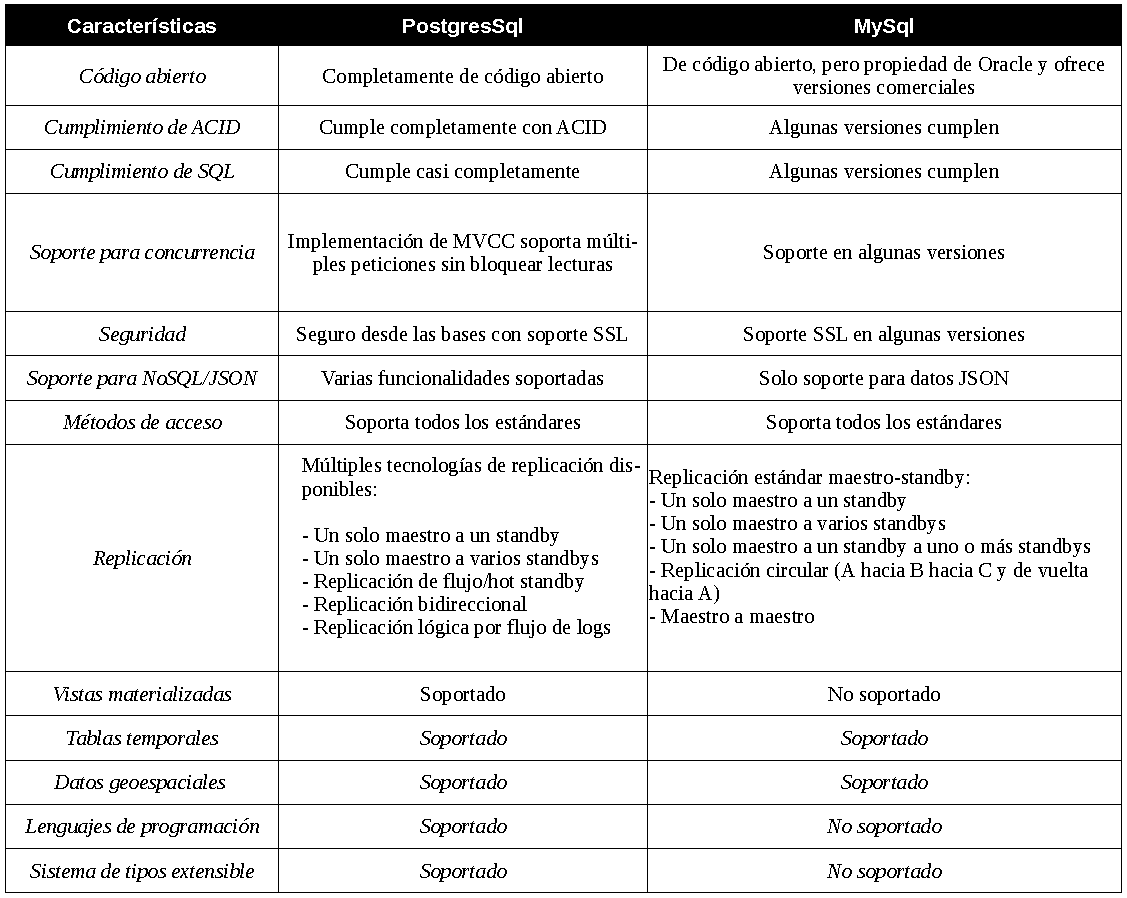
\includegraphics[scale=0.8]{figs/Tabla_Comparativa_DB.pdf}}
\caption{Tabla Comparativa de Motores de Base de Datos.}
\label{fig102}
\end{figure}
\renewcommand{\figurename}{Figura.}

\newpage
\subsubsection{Framewokrs para Testing}
\begin{itemize}
\item \textit{\textbf{PHPUnit}} \footnote{\textbf{PHPUnit}. \url{https://phpunit.de/}.}: \textit{es un entorno para realizar pruebas unitarias en el lenguaje de programación PHP. PHPUnit es un framework. Se creó con idea de que cuanto antes se detecten los errores en el código antes podrán ser corregidos. Este conocido framework para PHP nos permite crear y ejecutar juegos de tests unitarios de manera sencilla. Como todos los frameworks de pruebas unitarias, PHPUnit utiliza \textit{assertions} para verificar que el comportamiento de una unidad de código es el esperado.}

\item \textit{\textbf{Selenium}} \footnote{\textbf{PHPUnit}. \url{https://www.seleniumhq.org/}.}: \textit{es un entorno de pruebas de software para aplicaciones basadas en la web. Selenium provee una herramienta de grabar/reproducir para crear pruebas sin usar un lenguaje de scripting para pruebas (Selenium IDE). Incluye también un lenguaje específico de dominio para pruebas (Selanese) para escribir pruebas en un amplio número de lenguajes de programación populares incluyendo Java, C\#, Ruby, Groovy, Perl, Php y Python. Las pruebas pueden ejecutarse entonces usando la mayoría de los navegadores web modernos en diferentes sistemas operativos como Windows, Linux y OSX.}
\end{itemize}

\subsubsection{Manejadores de Dependencias}
\begin{itemize}
\item \textit{\textbf{Bower}} \footnote{\textbf{Bower}. \url{https://bower.io/}.}: \textit{es un complemento ideal para el desarrollo web. Es un sencillo programa que nos sirve para tener al día las dependencias de un proyecto para la web, en lo que respecta al desarrollo frontend, con Javascript o incluso CSS. Se trata de un programa basado en NodeJS que se ejecuta desde la consola y que tiene un sencillo API de comandos útiles para realizar tareas de mantenimiento y administración de paquetes necesarios para construir un proyecto web, concretamente la parte del lado del cliente. Con Bower es posible descargar y actualizar todo tipo de bibliotecas, frameworks, plugins, entre otros, sin tener que preocuparse por descargarlos e instalarlos.}
\end{itemize}

\subsubsection{Bibliotecas}
\begin{itemize}
\item \textit{\textbf{jQuery}} \footnote{\textbf{jQuery}. \url{https://jquery.com/}.}: \textit{es una biblioteca de JavaScript rápida, pequeña y rica en funciones. Entre otras cosas, se encarga del recorrido y manipulación de documentos HTML, manejo de eventos, animación, y Ajax mucho más simple con una API fácil de usar que funciona en una multitud de navegadores.}
\end{itemize}

\newpage
\subsubsection{Sistemas de Control de Versiones}
\begin{itemize}
\item \textit{\textbf{Git}} \footnote{\textbf{Git}. \url{https://git-scm.com/}.}: \textit{es un sistema de control de versiones distribuidas de código abierto y gratuito diseñado para manejar todo, desde proyectos pequeños a muy grandes, con velocidad y eficiencia. Es fácil de aprender y tiene una huella pequeña con un rendimiento increíblemente rápido. Supera a las herramientas de SCM como Subversion, CVS, Perforce y ClearCase con funciones como ramificación local barata, áreas de preparación conveniente y flujos de trabajo múltiples.}

\item \textit{\textbf{GitHub}} \footnote{\textbf{GitHub}. \url{https://github.com/}.}: \textit{es una plataforma de desarrollo inspirada en la forma en que trabajas. Desde el código abierto hasta el negocio, puede alojar y revisar códigos, administrar proyectos y crear software junto a millones de otros desarrolladores.}
\end{itemize}

\clearpage
\newpage
\chapter{Diseño del Sistema}
\section{Etapa 2 - Diseño del Sistema} \label{capitulo2}

\subsection{Introducción}
En el capítulo anterior se realizó un análisis que permitió definir las herramientas tecnológicas necesarias para lograr el objetivo de este proyecto. Por otro lado, se llevaron a cabo las tareas de elicitación de requerimientos, describiendo los procesos utilizados y los resultados obtenidos, siendo estos últimos los que definen qué es lo que el sistema debe hacer o dicho de otra manera, lo que el cliente espera del software. 

Por su parte, el presente capítulo busca transformar esos requerimientos recabados en una solución que satisfaga las demandas del cliente.

\subsection{Arquitectura del Sistema}
Teniendo en cuenta el objetivo general de este trabajo, el de desarrollar un Sitio Web, podemos estimar el tipo de arquitectura que será necesaria utilizar para llevar adelante el mismo. Este tipo de sistemas requiere la implementación del \textit{modelo cliente-servidor}. Este modelo se caracteriza por distribuir las tareas entre los proveedores de recursos o servicios, llamados servidores, y los demandantes, llamados clientes. Un cliente, en este caso un navegador web, realiza peticiones a un servidor, en este caso un programa, buscando obtener una respuesta.

En esta arquitectura, se cuenta con la importante ventaja de tipo organizativa debida a la centralización de la gestión de la información y la separación de responsabilidades, lo que facilita y clarifica el diseño del sistema.

La interfaz de usuario, es un aspecto importante a tener en cuenta dentro del proceso de desarrollo de sistemas interactivos. Si bien es posible desarrollar una interfaz de usuario partiendo desde cero, la solución más comúnmente usada, por razones de eficiencia y uniformidad, es apoyarse en arquitecturas que incluyen gestores de ventanas y a veces también cajas de herramientas (\textit{tool-box}). Esto implica que la interfaz estará íntimamente relacionada con el sistema de gestión de ventanas, por lo que se hace aconsejable una separación entre la aplicación y su interfaz, para conseguir los siguientes objetivos:
\begin{itemize}
\item \textit{\textbf{Portabilidad}}: \textit{permitir que una misma aplicación pueda ser utilizada en diferentes sistemas.}
\item \textit{\textbf{Reusabilidad}}: \textit{la separación incrementa la reusabilidad de los componentes.}
\item \textit{\textbf{Múltiples interfaces}}: \textit{flexibilidad para disponer de diferentes interfaces para la misma funcionalidad.}
\item \textit{\textbf{Personalización}}: \textit{adecuar las características de la interfaz a las preferencias y necesidades del usuario sin tener que modificar la aplicación.}
\end{itemize}

Siguiendo estos principios, se describen a continuación tres modelos de arquitectura cliente-servidor para la construcción de interfaces de usuario: el modelo \textit{Seeheim}, el \textit{Model–View–Controller} (Modelo-Vista-Controlador o MVC), y el PAC.

\begin{itemize}
\item \textit{\textbf{Seeheim}}: \textit{el modelo plantea la comunicación entre el usuario y la aplicación, de manera estructurada, en tres niveles}:
\begin{enumerate}
\item \textit{\textbf{El nivel de presentación}}: \textit{es la parte estática y visible de la interfaz que se comunica con el usuario y se construye sobre sistemas de ventanas y cajas de herramientas. Supondría el léxico de la interfaz.}

\item \textit{\textbf{El nivel de diálogo}}: \textit{es la parte dinámica que maneja los eventos o mensajes que se producen como consecuencia de las acciones del usuario, sobre la interfaz. Establece la comunicación entre el nivel de presentación y el nivel de aplicación, es decir, establece la relación entre los eventos y su correspondiente respuesta por parte del nivel de aplicación. Se podría equiparar a la sintaxis de la comunicación entre los otros dos niveles.}

\item \textit{\textbf{Interfaz de aplicación}}: \textit{es la parte de la aplicación que el usuario controla y que es visible para éste último. Equivaldría a la semántica de la aplicación.}
\end{enumerate}

\textit{La división en capas facilita el tratamiento de cada una por separado y además promueve la reutilización y la portabilidad, con lo que se posibilita el desarrollo rápido de prototipos, tarea fundamental para un diseñador.}

\item \textit{\textbf{MVC (Modelo Vista Controlador)}}: \textit{es un patrón de arquitectura de software que separa, los datos y la lógica de negocio de una aplicación, de la representación y la gestión de los eventos y las comunicaciones. Para ello MVC propone la construcción de tres componentes: el \textit{modelo}, la \textit{vista} y el \textit{controlador}. Es decir, por un lado define componentes para la representación de la información, y por otro la interacción del usuario.}

\textit{El modelo es la representación de la información con la cual el sistema opera, por lo tanto gestiona todos los accesos a dicha información, implementando también los privilegios de acceso que se hayan descrito en las especificaciones de la aplicación (lógica de negocio). Envía a la vista aquella parte de la información que en cada momento se le solicita sea mostrada. Las peticiones de acceso o manipulación de información llegan al modelo a través del controlador. El controlador responde a eventos, usualmente acciones del usuario, e invoca peticiones al modelo cuando se hace alguna solicitud sobre la información (por ejemplo, editar un documento o un registro en una base de datos). También puede enviar comandos a su vista asociada si se solicita un cambio en la forma en que se presenta el modelo (por ejemplo, desplazamiento o scroll por un documento o por los diferentes registros de una base de datos). Por tanto, se podría decir que el controlador hace de intermediario entre la vista y el modelo.} 

\textit{Por último, la vista presenta el modelo (información y lógica de negocio) en un formato adecuado para interactuar con el usuario, para lo cual requiere de dicho modelo la información que debe presentar como salida.}

\newpage
\item \textit{\textbf{PAC (Presentación-Abstracción-Control)}}: \textit{se apoya en tres pilares básicos}:
\begin{itemize}
\item \textit{\textbf{Presentación}: gestiona las entradas/salidas.}
\item \textit{\textbf{Abstracción}: representa la semántica de la aplicación.}
\item \textit{\textbf{Control}: gestiona el diálogo y la correspondencia entre la aplicación y presentación.}
\end{itemize}
\end{itemize}

Como puede apreciarse, PAC es una arquitectura bastante similar a MVC, aunque existen diferencias entre ellas. PAC agrupa la entrada/salida en la presentación, mientras que en MVC la vista se ocupa de la salida y el controlador de la entrada. Además, PAC introduce el control como mecanismo para mantener la consistencia entre la abstracción y la presentación, lo que en MVC no supone una tarea asignada de antemano. Por último, PAC no ha nacido vinculado a ningún entorno de programación, como le ocurre a MVC, aunque ambos lleven a una aproximación orientada a objetos.

Luego de analizar los patrones de diseño presentados, se llega a la conclusión de que tanto MVC como PAC proveen los medios necesarios para lograr una aplicación modular, escalable y fácil de mantener. En ambos casos se tiene a la interfaz de usuario separada de la lógica de negocio y se propone la organización de la información a través de modelos o abstracciones.

%Es importante aclarar que la selección de la arquitectura es un proceso que no puede disociarse de la selección tecnológica. Por eso, además de analizar las ventajas operacionales de los distintos modelos presentados, se debe tener en cuenta la disponibilidad de tecnologías que permitan implementarlos. Este es un punto en el que MVC se supera a PAC, ya que su enorme popularidad ha impulsado el surgimiento de un gran número de frameworks y herramientas pensadas para implementar este tipo de patrón arquitectónico, facilitando y agilizando el desarrollo de aplicaciones web.

Con lo expuesto anteriormente se cuenta con las herramientas suficientes para definir el patrón de diseño a utilizar para el desarrollo del sistema, el mismo será MVC.

\subsection{Descomposición del Sistema en Módulos}
El objetivo detrás de la descomposición del sistema en en módulos es el de generar subsistemas abstractos lo suficientemente pequeños que permitan independizarlos unos de otros de forma tal que el abordaje de la solución pueda ser abordado de manera mas sencilla.

En ingeniería de software, un \textit{Diagrama de Clases} en Lenguaje Unificado de Modelado (UML) es un tipo de diagrama de estructura estática que describe al sistema mostrando sus clases, atributos, operaciones (o métodos), y las relaciones entre los objetos. En la Fig. \eqref{fig201} se puede apreciar el diagrama.

Los diagramas son el nexo entre los requerimientos del sistema y el sistema propiamente dicho. Es decir, que cuanto mas pueda describirse la estructura y lógica del sistema a través de estos modelos UML, mejor aún será el nivel de detalle alcanzado y será mas fácil abordar el problema.

\begin{figure}[tbhp]
\centerline{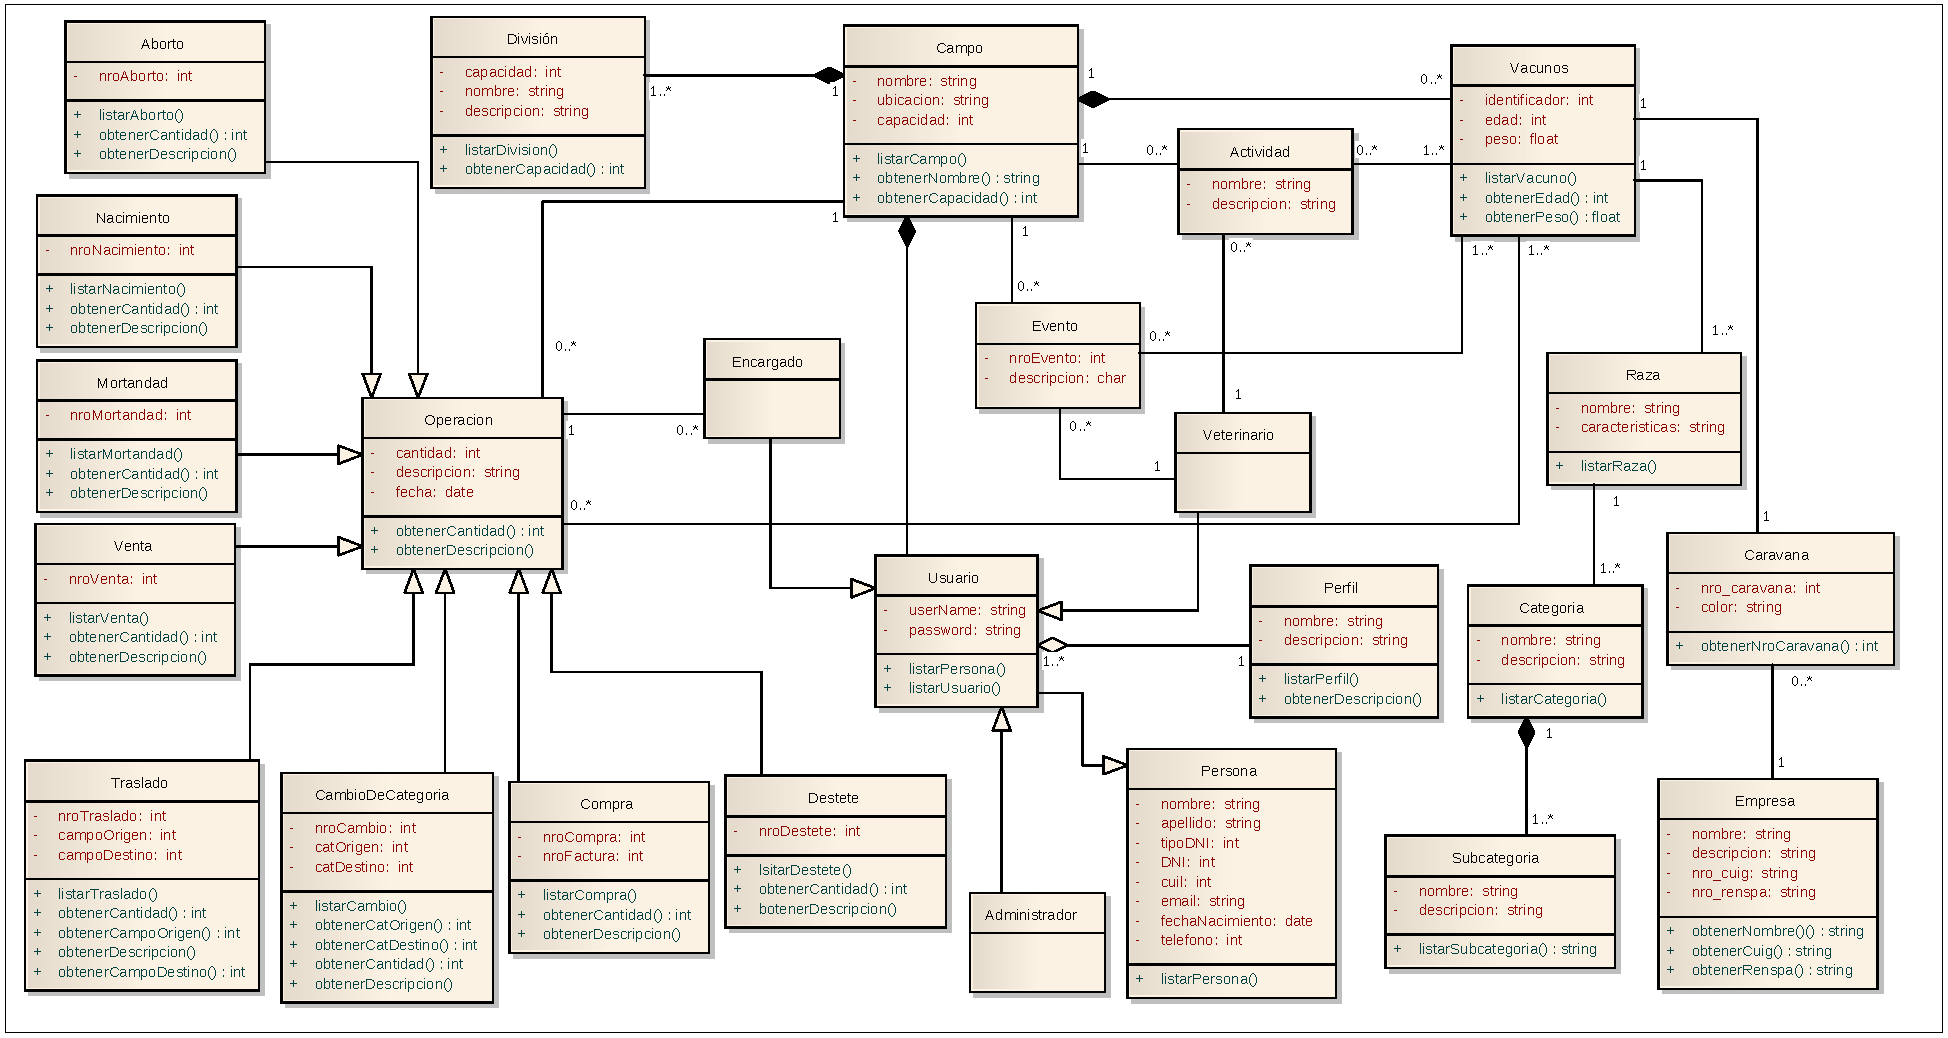
\includegraphics[scale=0.55]{figs/FINAL_Diagrama_Clases.pdf}}
\caption{Diseño del Sistema: Diagrama de Clases.}
\label{fig201}
\end{figure}

\clearpage
\newpage
\subsection{Diseño físico de la Base de Datos}
Tomando referencia del diagrama de clases se diseño la base de datos. El diagrama físico de la base de datos puede apreciarse en la Fig. \eqref{fig202}. En él, se encuentran los atributos y relaciones entre las distintas tablas. Los elementos utilizados para representar estas relaciones son los denominados Foreign Key (FK) que intentan esbozar la relación de existencia de una instancia de una clase, en otra. Por otro lado, dentro de una misma tabla, la forma de identificar e individualizar cada registro se hace bajo la utilización de lo que se denomina Primary Key (PK). Visualmente, los atributos PK poseen un asterisco (*) a su izquierda mientras que los atributos FK poseen en su nombre dicha propiedad. 

\begin{figure}[tbhp]
\centerline{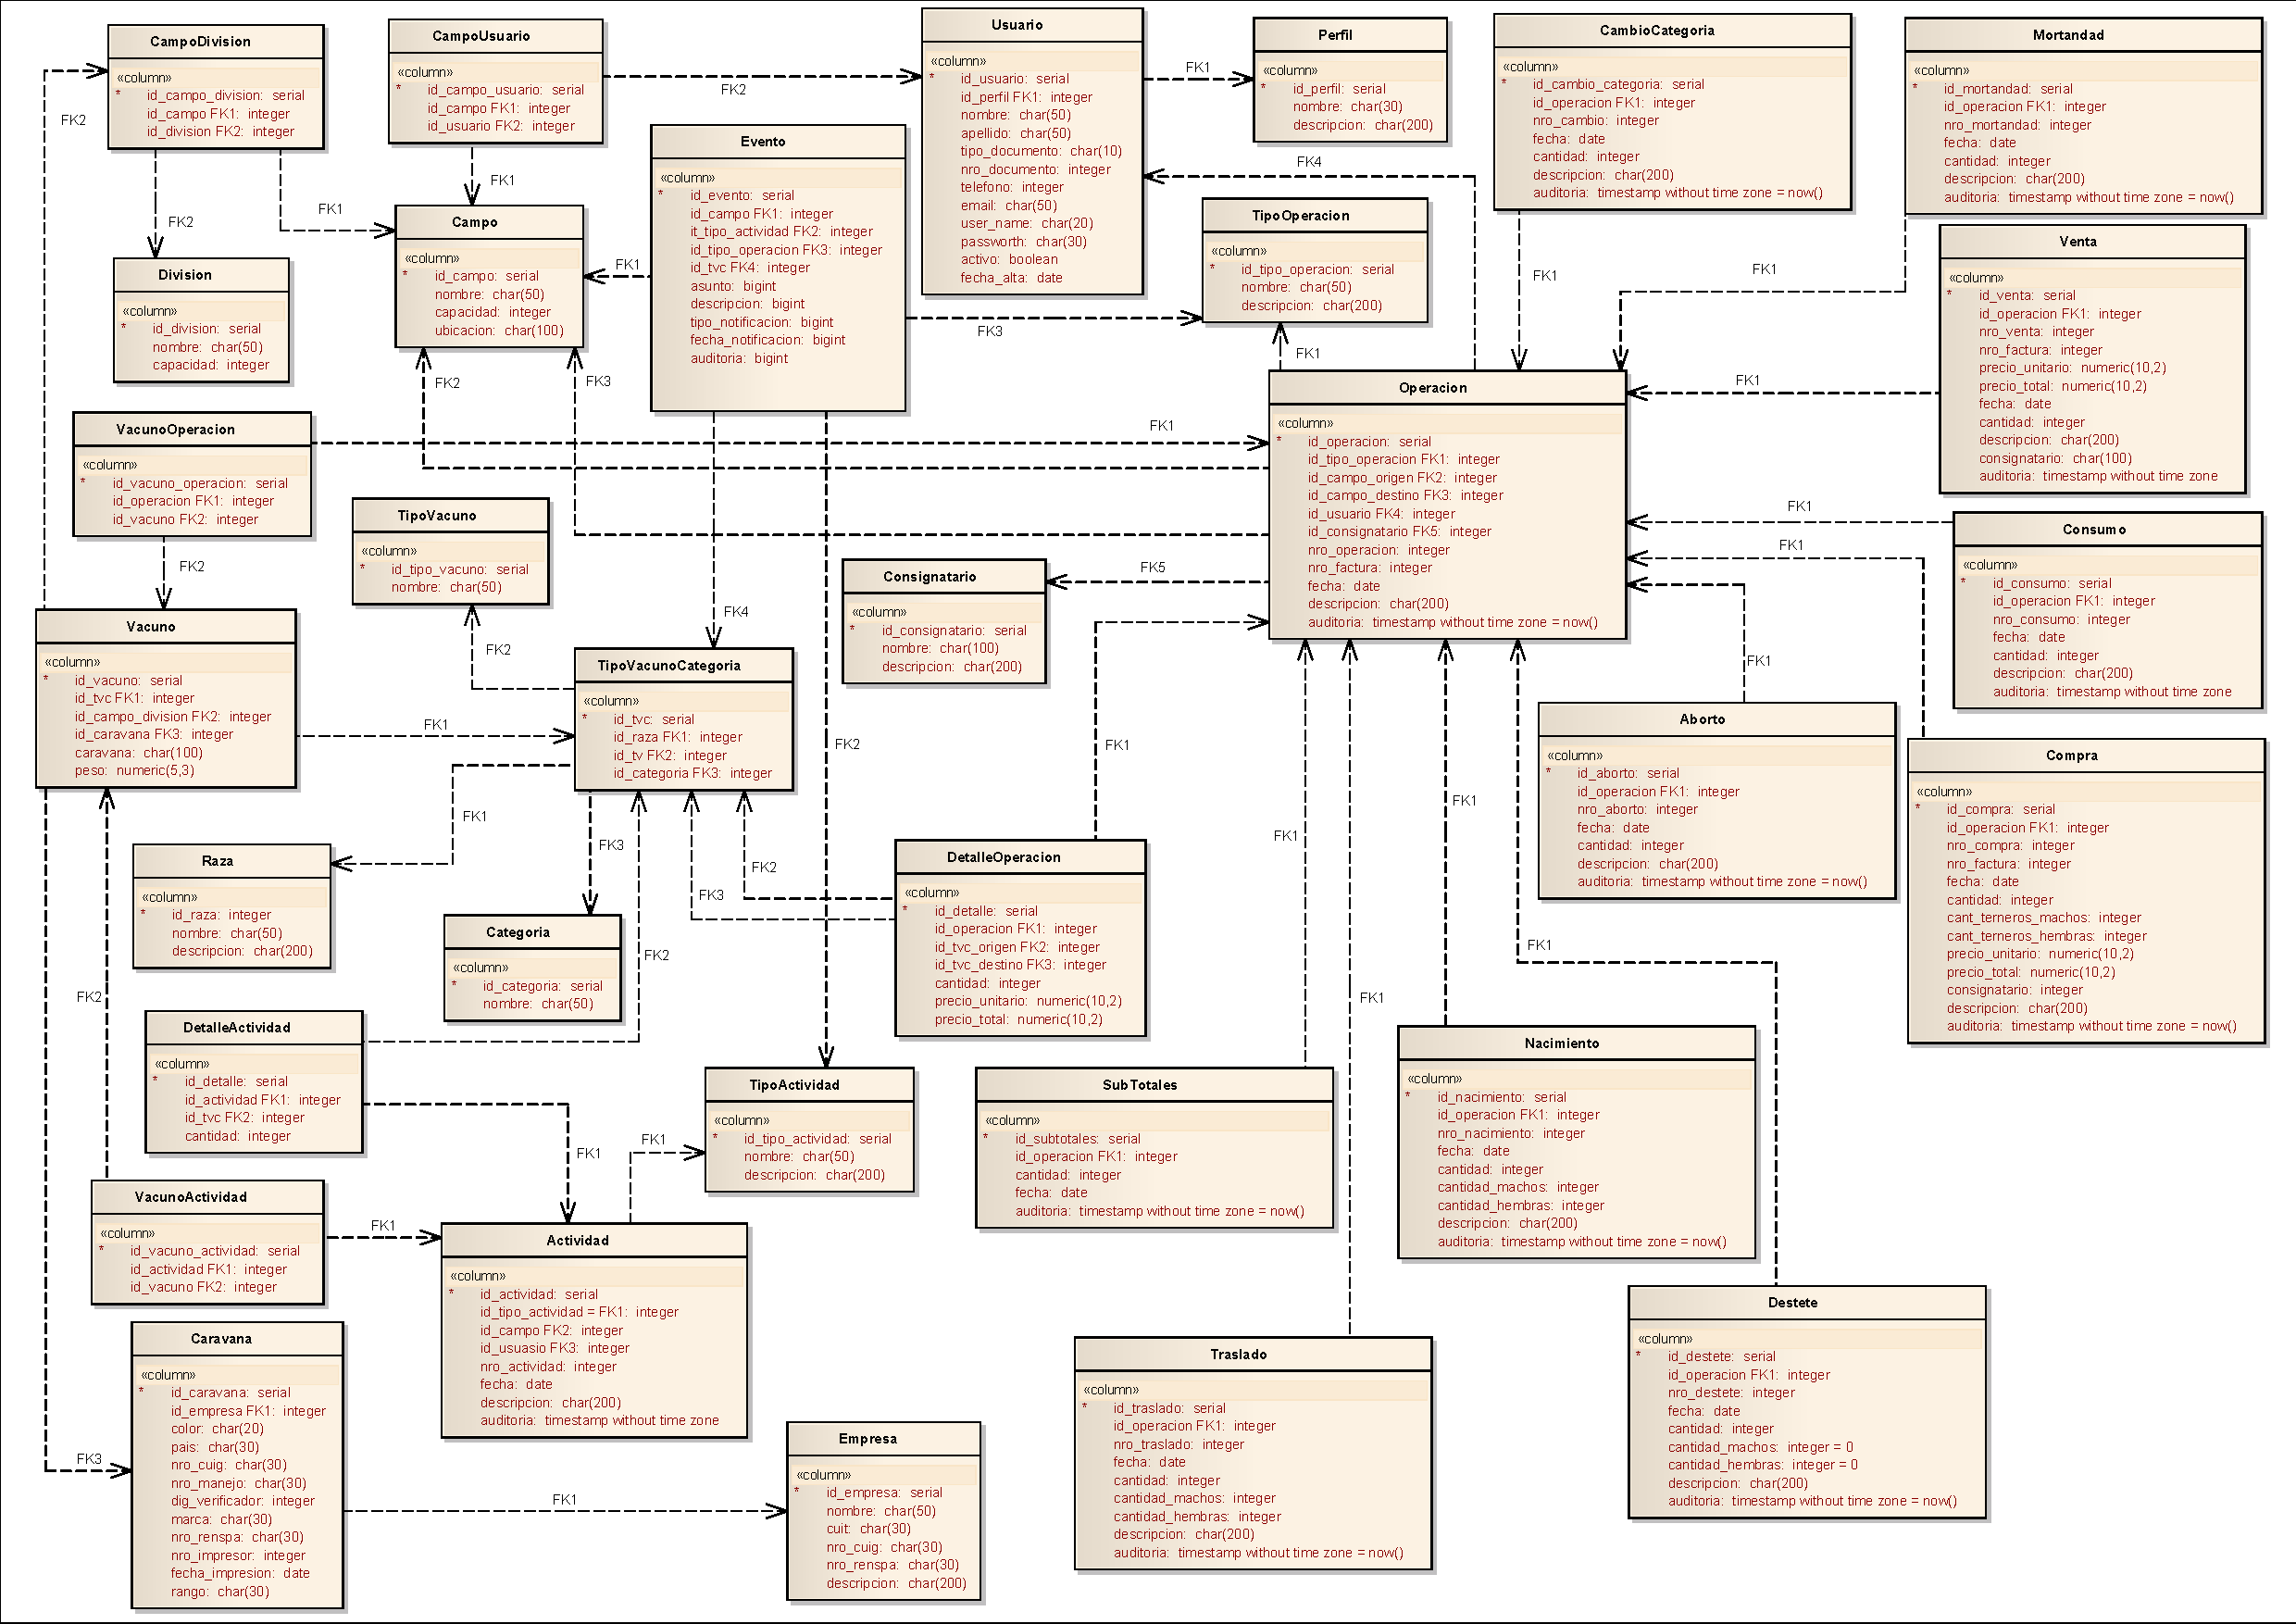
\includegraphics[scale=0.4]{figs/FINAL_Diagrama_Fisico_DB.pdf}}
\caption{Diseño del Sistema: Diseño Físico de la Base de Datos.}
\label{fig202}
\end{figure}

\newpage
\subsection{Diseño de la Interfaz Gráfica de Usuario}
En la vida cotidiana interactuamos constantemente con Interfaces Gráficas de Usuario (GUI por su nombre en inglés Graphical User Interface) no sólo al usar una computadora sino también en objetos de uso diario como el celular, el cajero automático, etc. entre muchas otras cosas. La interfaz tiene un papel fundamental para que el producto sea o no competitivo. El producto no será exitoso si el usuario no consigue concretar una acción (por ejemplo:  una transacción económica), o no entiende la secuencia de pasos a seguir, o cuando no encuentra con facilidad cómo concretar la acción que necesita (por ejemplo: realizar una compra) o cuando no considera atractivo el diseño de la aplicación que está utilizando.

La Interfaz de Usuario es la parte del software que las personas pueden ver, oír, tocar, hablar; es decir, donde   se pueden entender. Contiene, esencialmente, dos componentes: la \textit{entrada} y la \textit{salida}. La entrada es cómo una persona le comunica sus necesidades o deseos al sistema. La salida es la forma en que la computadora transmite los resultados a lo solicitado por el usuario.

En la actualidad la GUI es parte fundamental de cualquier aplicación, y por lo tanto tiene tanta importancia como el desarrollo de la aplicación en sí.

Principios de diseño de interfaz gráfica de usuarios, según Sommerville:
\begin{itemize}
\item \textit{\textbf{Familiaridad del usuario}: significa que la interfaz debe utilizar términos e imágenes conocidos por el usuario; y los objetos que manipula el sistema deben estar relacionados con el ámbito de trabajo.}

\item \textit{\textbf{Uniformidad de la Interfaz}: significa que tanto comandos como menús deben tener el mismo formato. Las Interfaces uniformes reducen el tiempo de aprendizaje.}

\item \textit{\textbf{Mínima sorpresa}: el comportamiento del sistema no debe mostrar situaciones inesperadas. Ante éste tipo de situaciones el usuario puede mostrar irritabilidad, por lo tanto perder interés en utilizar la aplicación.}

\item \textit{\textbf{Recuperación de estados}: éste es uno de los principios más importantes al diseñar una Interfaz. Es inevitable cometer errores, por lo tanto el sistema le debe proporcionar al usuario la manera de subsanarlos o volver a estados anteriores. Éste principio involucra varias acciones como pedir al usuario que confirme acciones destructivas, que el usuario pueda deshacer, etc.}
 
\item \textit{\textbf{Guía de usuarios}: la Interfaz debe proporcionar al usuario asistencia, ayuda. No sólo cuando se cometen errores sino también cuando no se sabe qué hacer o cómo hacer alguna tarea. Esta ayuda debe estar integrada al sistema (algunas además ofrecen ayuda on line) y debe ser clara cuando el usuario la requiera, sin saturar con información.}
 
\item \textit{\textbf{Diversidad de usuarios}: se debe tener en cuenta los diferentes usuarios que pueden utilizar la aplicación. Aquellos casuales, que necesitan que los guíen, y aquellos que podrían usarla constantemente los cuales necesitarán trabajar con métodos abreviados, tan rápido como sea posible. Además se podría incluir recursos para mostrar diferentes tamaños de texto, reemplazar sonido por texto y al revés, modificar tamaño de botones, etc. Esto refleja la noción de Diseño Universal, principio de diseño cuyo objetivo es evitar excluir usuarios.}
\end{itemize}

\subsubsection{Aspectos fundamentales a la hora de Diseñar la Interfaz}
A continuación se describen aquellos aspectos que han sido considerados a la hora de realizar el diseño de la Interfaz Gráfica de Usuario:

\begin{itemize}
\item \textit{\textbf{Diseño adaptable}}: \textit{el diseño web adaptable (también conocido como diseño web adaptativo o responsivo), es una filosofía de diseño y desarrollo cuyo objetivo es adaptar la apariencia de las páginas web al dispositivo que se esté utilizando para visitarlas.}

\textit{La ventaja de utilizar un diseño adaptable radica en que con una sola versión en \textbf{HTML} y \textbf{CSS} se pueden cubrir todas las resoluciones de pantalla, con lo que el sitio web estará optimizado para distintos dispositivos y resoluciones.}

\begin{figure}[tbhp]
\centerline{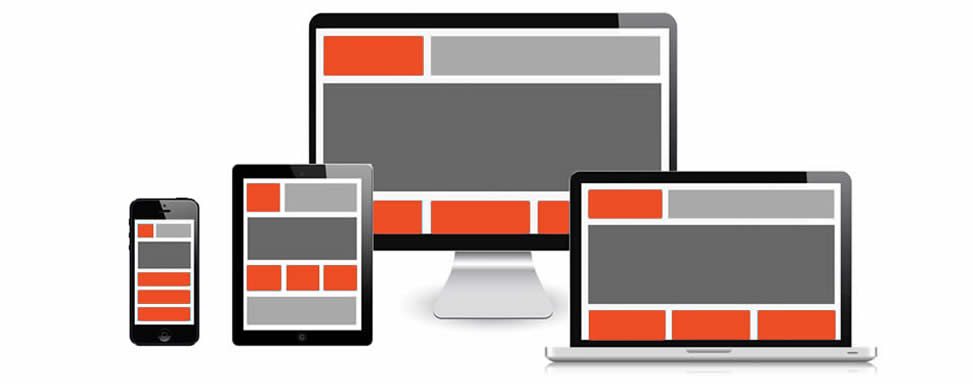
\includegraphics[scale=0.3]{figs/responsive_2.jpg}}
\caption{Diseño del Sistema: Diseño Adaptable.}
\label{fig203}
\end{figure}

\item \textit{\textbf{Compatibilidad}: el objetivo de la compatibilidad web es lograr que una aplicación se vea de la misma manera en todos los navegadores y que funcione correctamente en cada uno de ellos. Para conseguir la compatibilidad web se utilizaron tablas de compatibilidad (quirksmode.org, w3c.org) donde se pueden realizar consultas acerca de la compatibilidad de cada recurso utilizado con los distintos navegadores. Por otro lado, se validó el código de manera automática con la herramienta de validación de lenguaje de marcado del W3C (World Wide Web Consortium).}

\item \textit{\textbf{Usabilidad}: la usabilidad web es el grado de facilidad de uso que tiene una página web para los visitantes que entran e interactúan con ella. Un sitio web con buena usabilidad es aquel que permite a los usuarios una interacción sencilla, intuitiva, agradable y segura.}
    
\textit{Para lograr buena usabilidad es necesario combinar con habilidad una serie de factores de diversos tipos: tecnológicos, de diseño, de contenidos, etc. Jakob Nielsen \footnote{\textbf{Jakob Nielsen}. \url{https://www.nngroup.com/articles/ten-usability-heuristics/}.} (Enero,1995) formuló diez principios sobre usabilidad de páginas web:}

\begin{enumerate}
\item \textit{\textbf{Visibilidad del estado del sistema}: siempre se debe tener informado al usuario de lo que está pasando en nuestra web y ofrecerle una respuesta en el menor tiempo posible.}

\item \textit{\textbf{Relación entre el sistema y el mundo real}: el sistema tiene que ``habla'' el lenguaje del usuario con palabras o frases que a éste le sean familiares y que pueda reconocer con facilidad. La información tiene que mostrarse con un orden lógico y las imágenes o iconos usados tienen que ser claros, sin darle la posibilidad al usuario de equivocarse.}

\item \textit{\textbf{Control y libertad del usuario}: a veces, un usuario se equivoca, es normal. Tenemos que darle al usuario la posibilidad de subsanar el error y no sentirse frustrado por no poder realizar algo.}

\item \textit{\textbf{Consistencia y estándares}: se deben tener en cuenta los convenios establecidos para ciertos iconos. Por ejemplo, las líneas horizontales que indican el menú desplegable. En la versión responsive es mejor implementar este icono como menú desplegable y no utilizar otro, ya que el usuario puede llegar a no entender dicho icono.}

\item \textit{\textbf{Prevención de errores}: se debe prevenir cualquier error que pueda cometer el usuario. Y dado el caso de que este cometa uno, tenemos que poner a su alcance todas las opciones posibles para poder corregirlo. La opción de autocompletar es un buen ejemplo de este principio de usabilidad web.}

\item \textbf{Reconocer antes que recordar}: siempre es mejor reconocer que obligar al usuario a memorizar acciones u objetos para que pueda cumplir su objetivo. Ayudar al usuario a no memorizar en importante a la hora de pensar en el diseño de un sitio web.

\item \textit{\textbf{Flexibilidad y eficiencia de uso}: el sitio web debe estar preparado para todo tipo de usuario, desde los más novatos hasta los más experimentados. Si conseguimos que cualquiera pueda navegar por nuestra web logramos flexibilidad. Y si tenemos opciones para los más experimentados obtenemos eficiencia.}

\item \textbf{Diseño estético y minimalista}: las páginas web no deben contener información innecesaria, distrae al usuario y puede llegar a molestar en la navegación.

\item \textit{\textbf{Ayudar a los usuarios a reconocer, diagnosticar y corregir los errores}: todos los errores que puedan ocurrir en el sitio web deben estar expresados en un lenguaje entendible por todos, no por códigos.}

\item \textit{\textbf{Ayuda y documentación}: con estos principios se intenta siempre que el usuario no tenga que usar documentos de ayuda para poder navegar o utilizar una aplicación. Aun así, siempre tenemos que dar al usuario  la posibilidad de tener un pequeño manual de funcionamiento. Esta ayuda debe ser fácil de localizar, definir los pasos claramente y no ser muy extensa.}
\end{enumerate}
\end{itemize}

A continuación se muestran a modo de ejemplo unas ilustraciones de páginas que formarán parte del sitio web. Cabe aclarar que las mismas son meramente ilustrativas, ya que al no haber comenzado de manera formal con el desarrollo del sitio, no es posible representar de manera precisa el contenido de las mismas.

En la Fig. \eqref{fig204} se muestra la pantalla de \textit{Inicio de Sesión} mientras que en la Fig. \eqref{fig205} se muestra el formulario mediante el cual se procede a registrar la \textit{Compra de Vacunos}. Ambas están representadas en dispositivos que poseen diferentes características de resolución de pantalla esbozando, de esta manera, la adaptabilidad del sitio.

\begin{figure}[tbhp]
\centerline{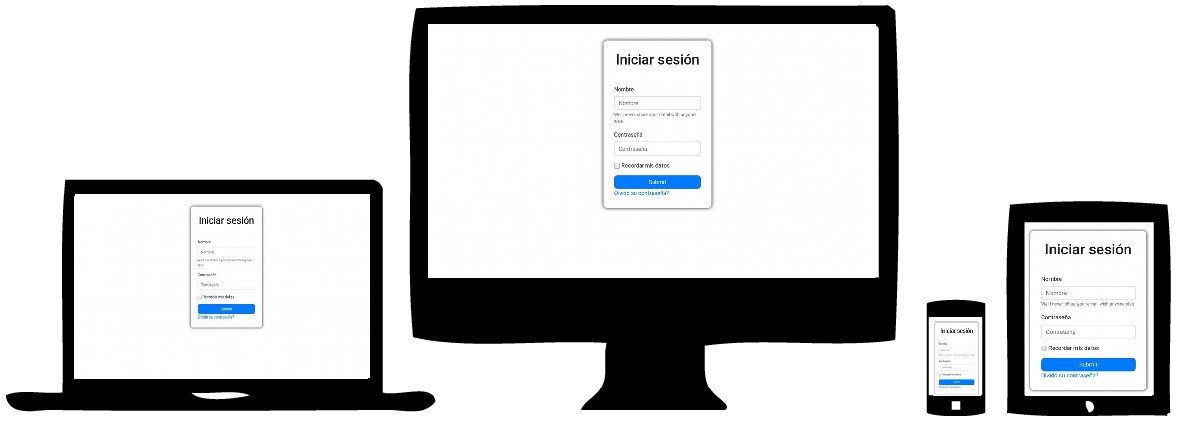
\includegraphics[scale=0.7]{figs/loginForm.pdf}}
\caption{Diseño del Sistema: Inicio de Sesión.}
\label{fig204}
\end{figure}

\begin{figure}[tbhp]
\centerline{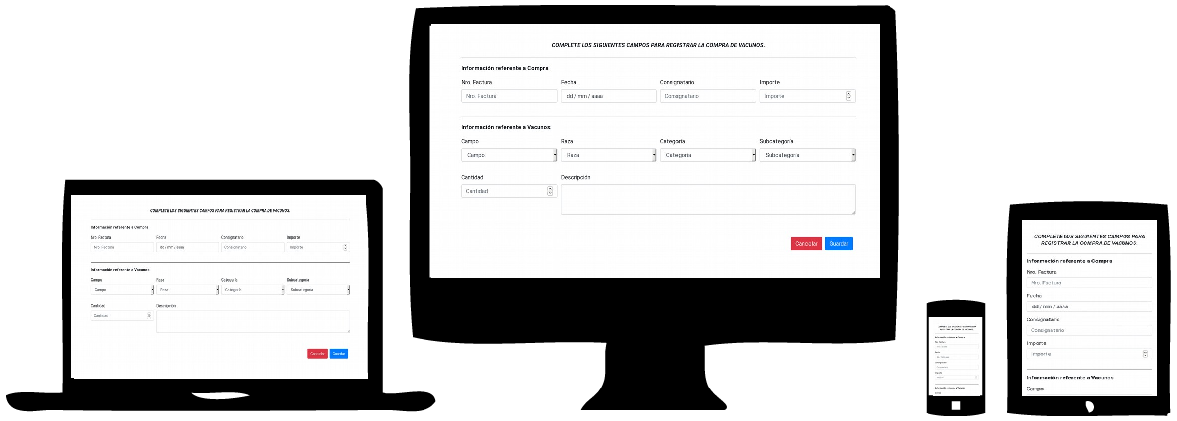
\includegraphics[scale=0.7]{figs/compraForm.pdf}}
\caption{Diseño del Sistema: Formulario de Compra.}
\label{fig205}
\end{figure}

\chapter{Desarrollo}

\chapter{Pruebas}

\chapter{Conclusiones y Trabajos Futuros}
%%%%%%%%%%%%%%%%%%%%%%%%%%%%%%%%%%%%%%%%%% FIN DEL DOCUMENTO %%%%%%%%%%%%%%%%%%%%%%%%%%%%%%%%%%%%%%%%%

%%%%%%%%%%%%%%%%%%%%%%%%%%%%%%%%%%%%%%%%%%%%% APÉNDICE DE CASOS DE USO %%%%%%%%%%%%%%%%%%%%%%%%%%%%%%%%%%%%%%%%%%%
\clearpage
\newpage
\section{Apéndice - Casos de Uso}\label{Ap}

\subsection{Diagramas de Casos de Uso}\label{ApDCU}
\begin{figure}[tbhp]
\centerline{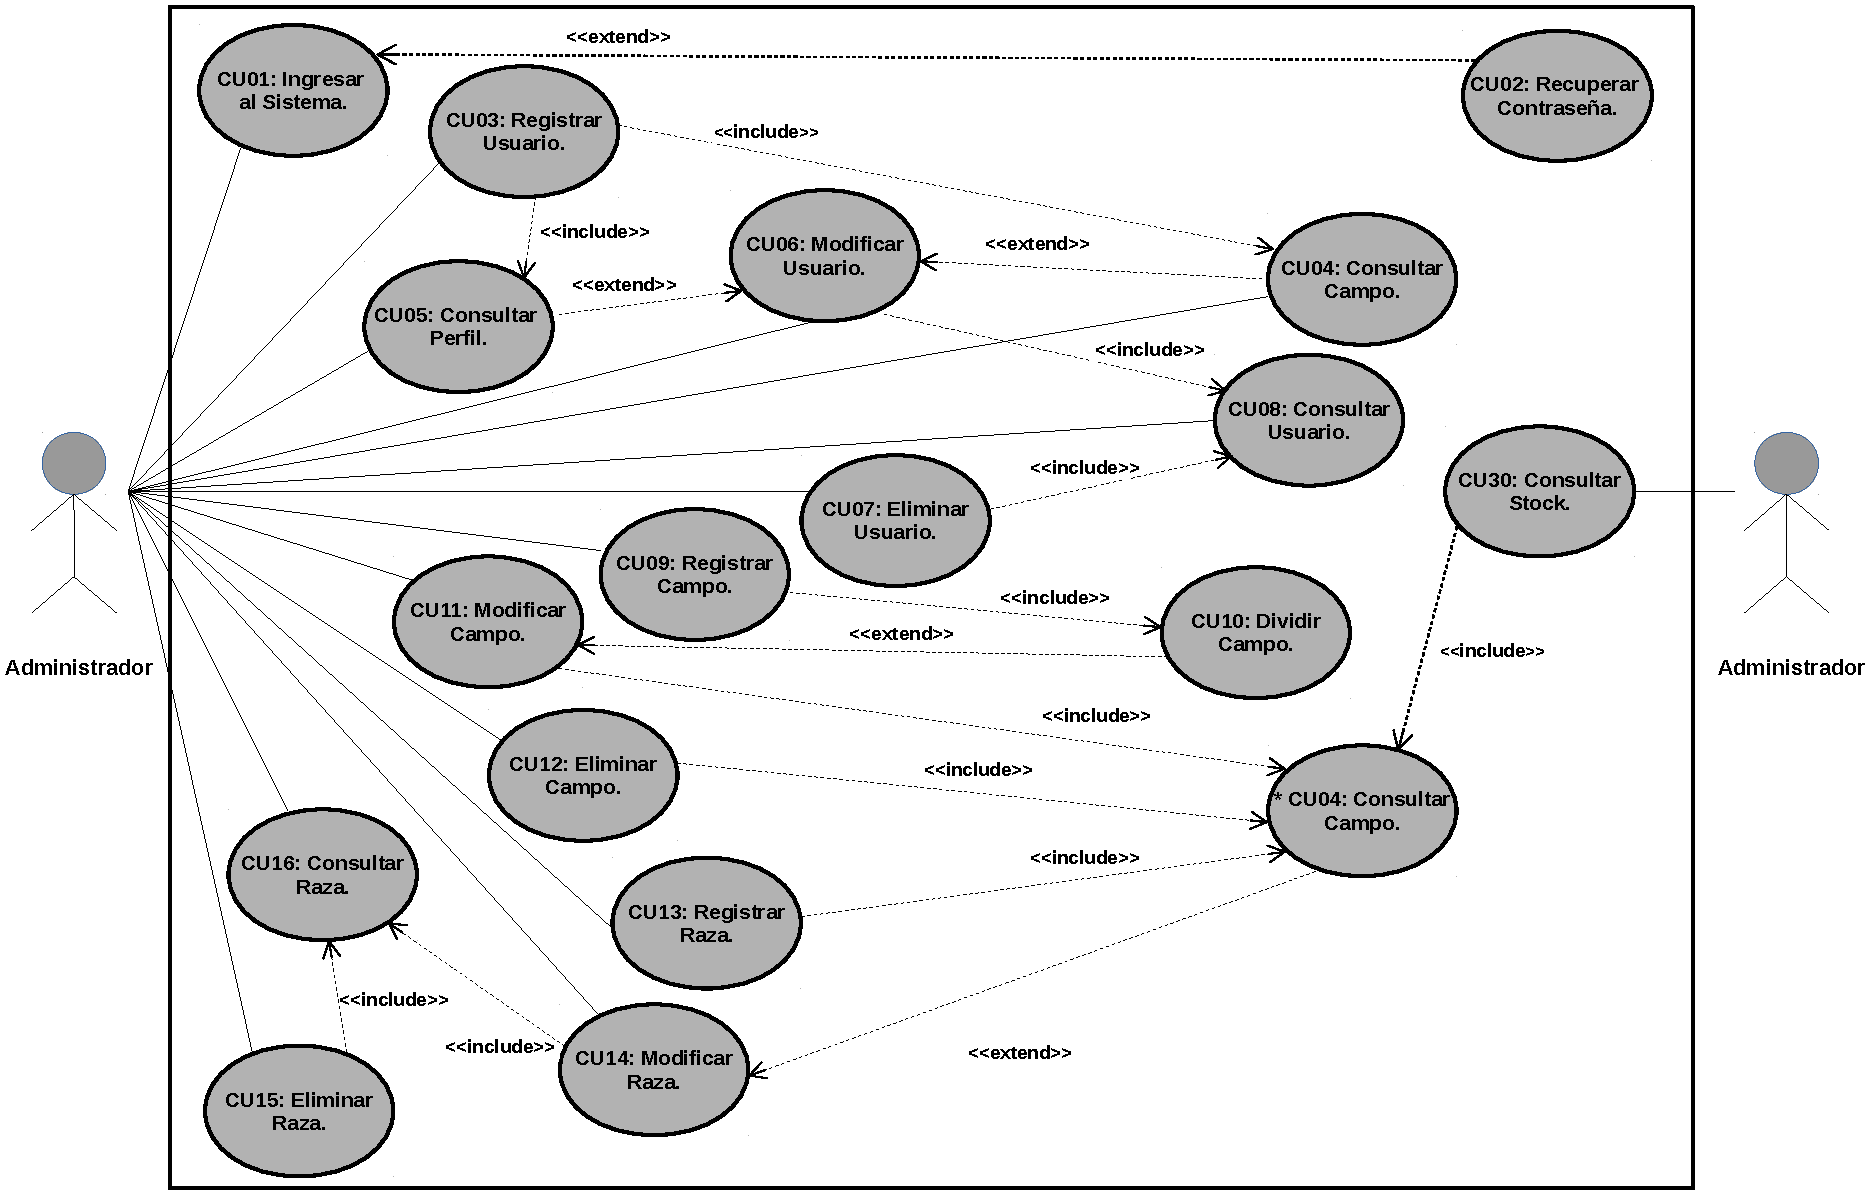
\includegraphics[scale=0.5]{figs/Diagrama_CU_Administrador.pdf}}
\caption{Diagrama de Casos de Uso del Actor \textbf{Administrador}.}
\label{Ap101}
\end{figure}

\begin{figure}[tbhp]
\centerline{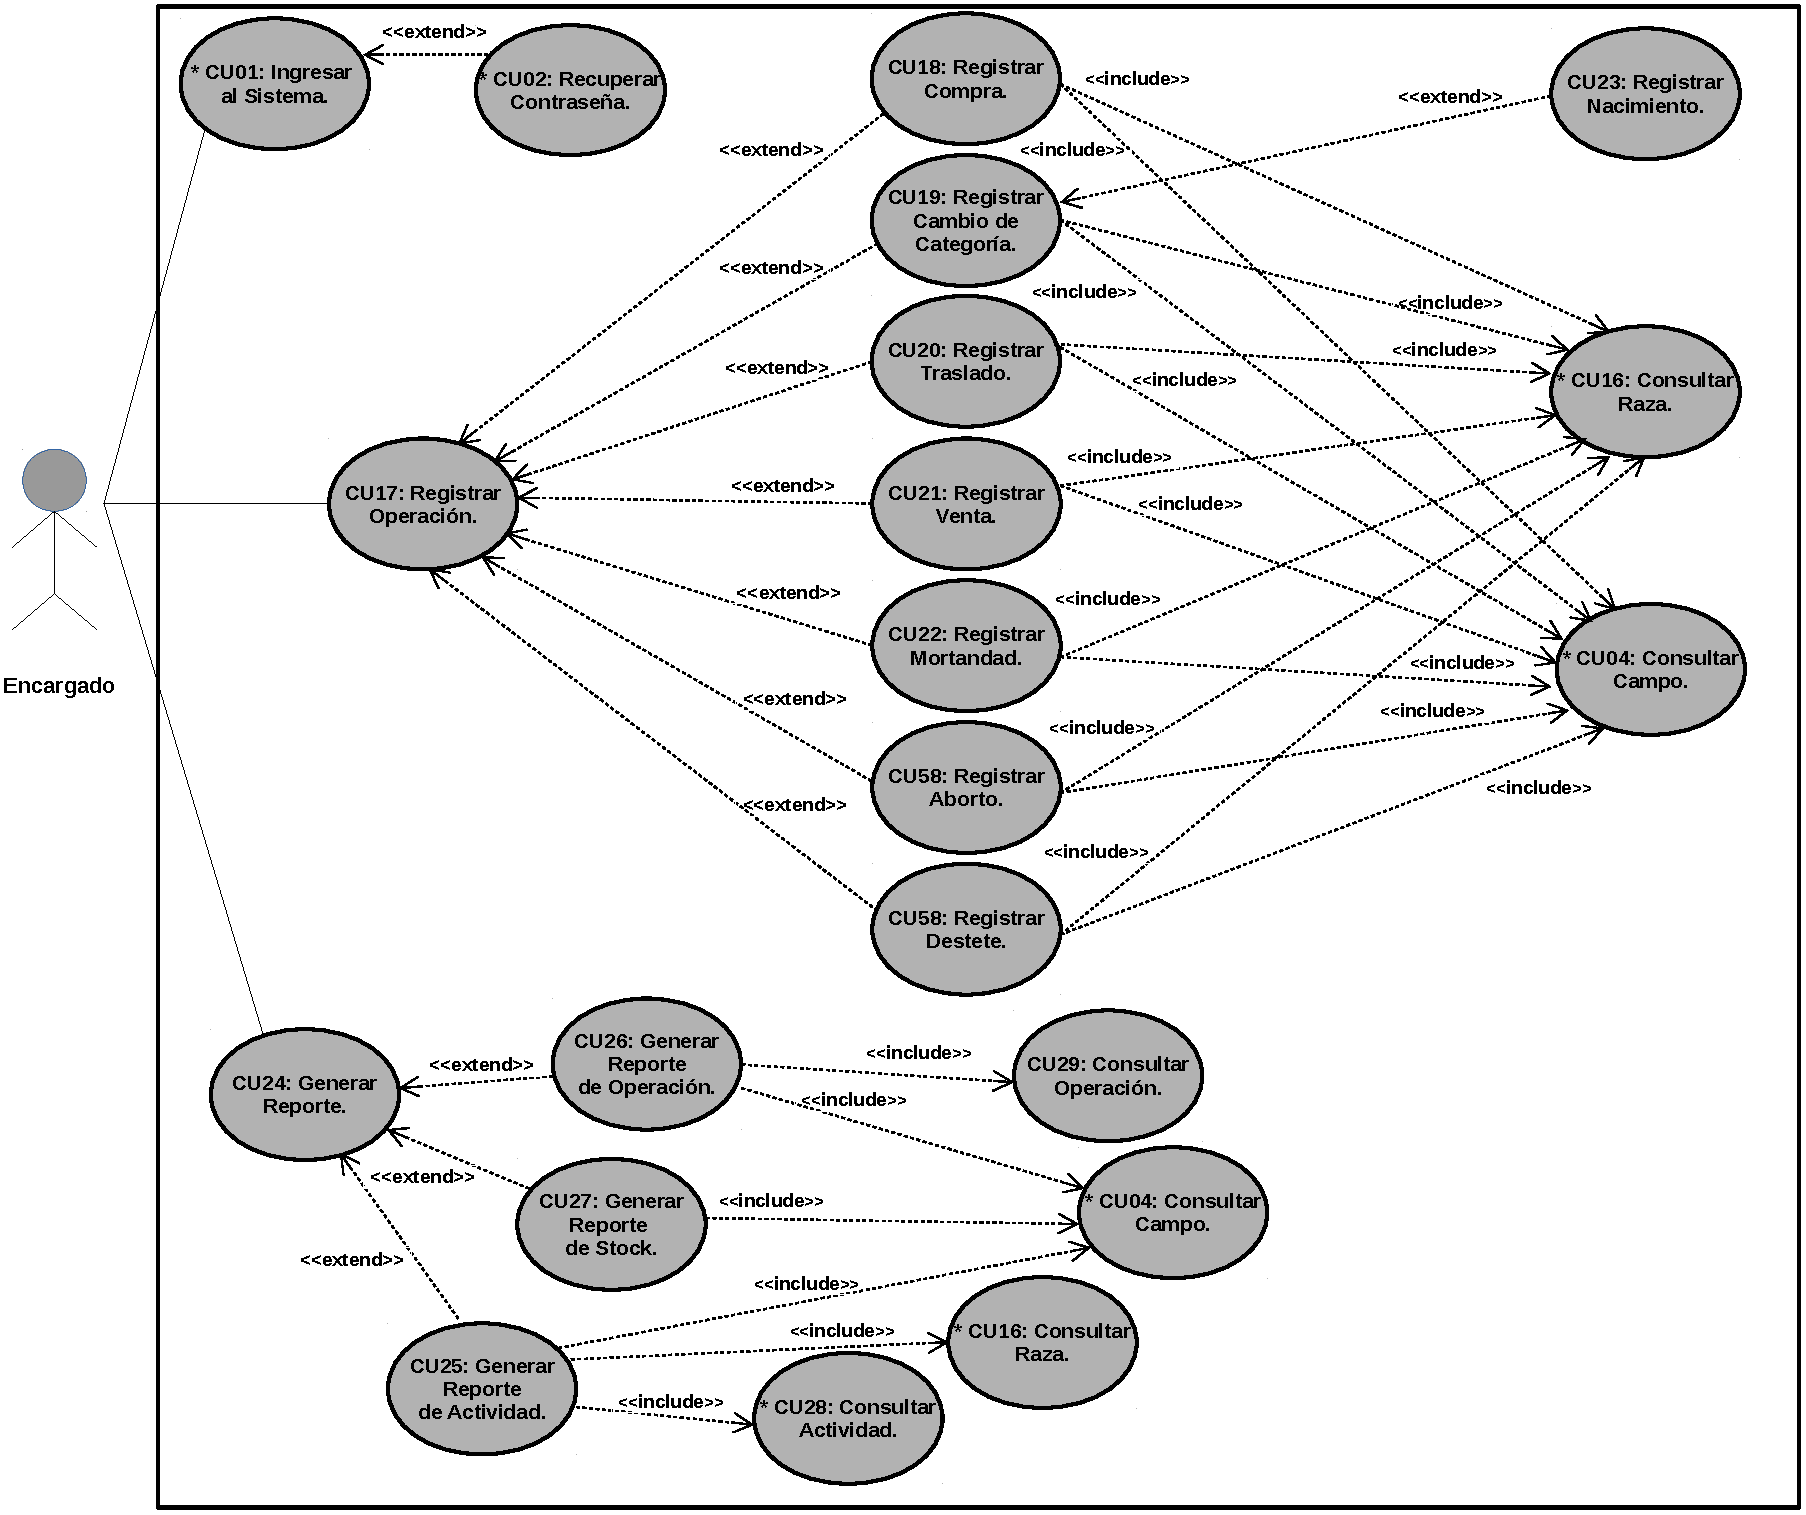
\includegraphics[scale=0.5]{figs/Diagrama_CU_Encargado.pdf}}
\caption{Diagrama de Casos de Uso del Actor \textbf{Encargado} - Parte 1.}
\label{Ap102}
\end{figure}

\begin{figure}[tbhp]
\centerline{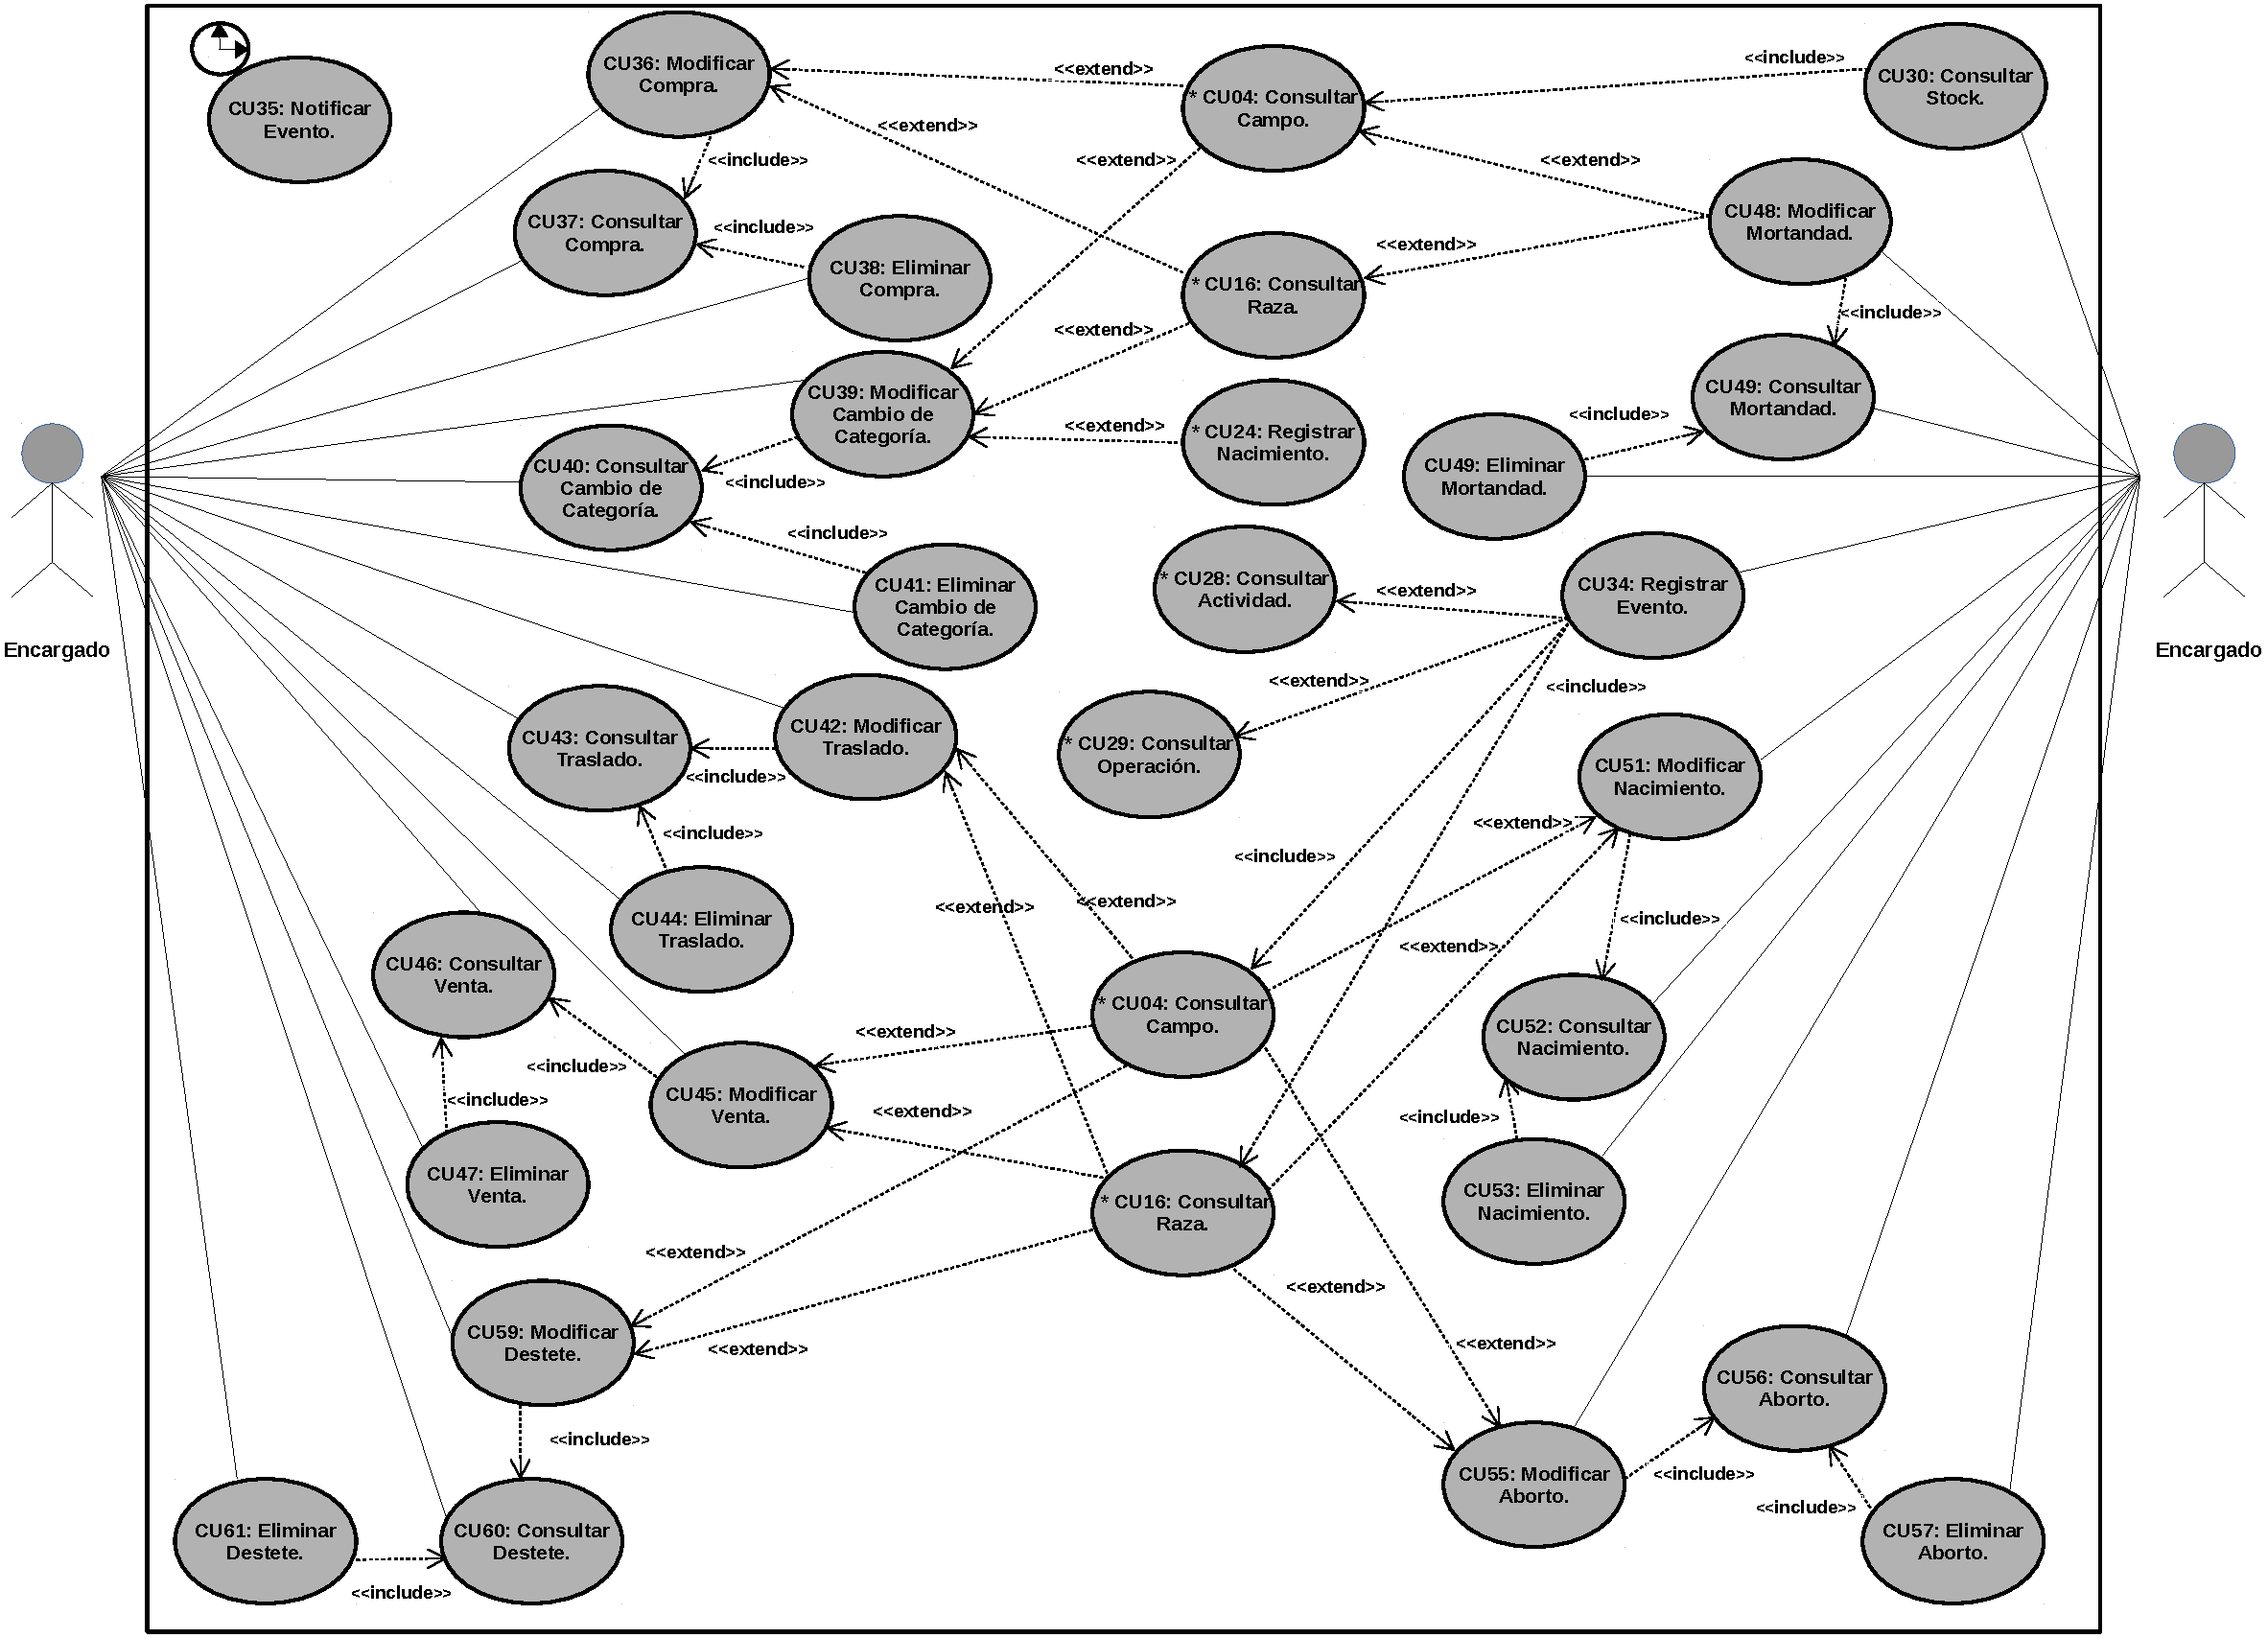
\includegraphics[scale=0.5]{figs/Diagrama_CU_Restantes.pdf}}
\caption{Diagrama de Casos de Uso del Actor \textbf{Encargado} - Parte 2.}
\label{Ap103}
\end{figure}

\begin{figure}[tbhp]
\centerline{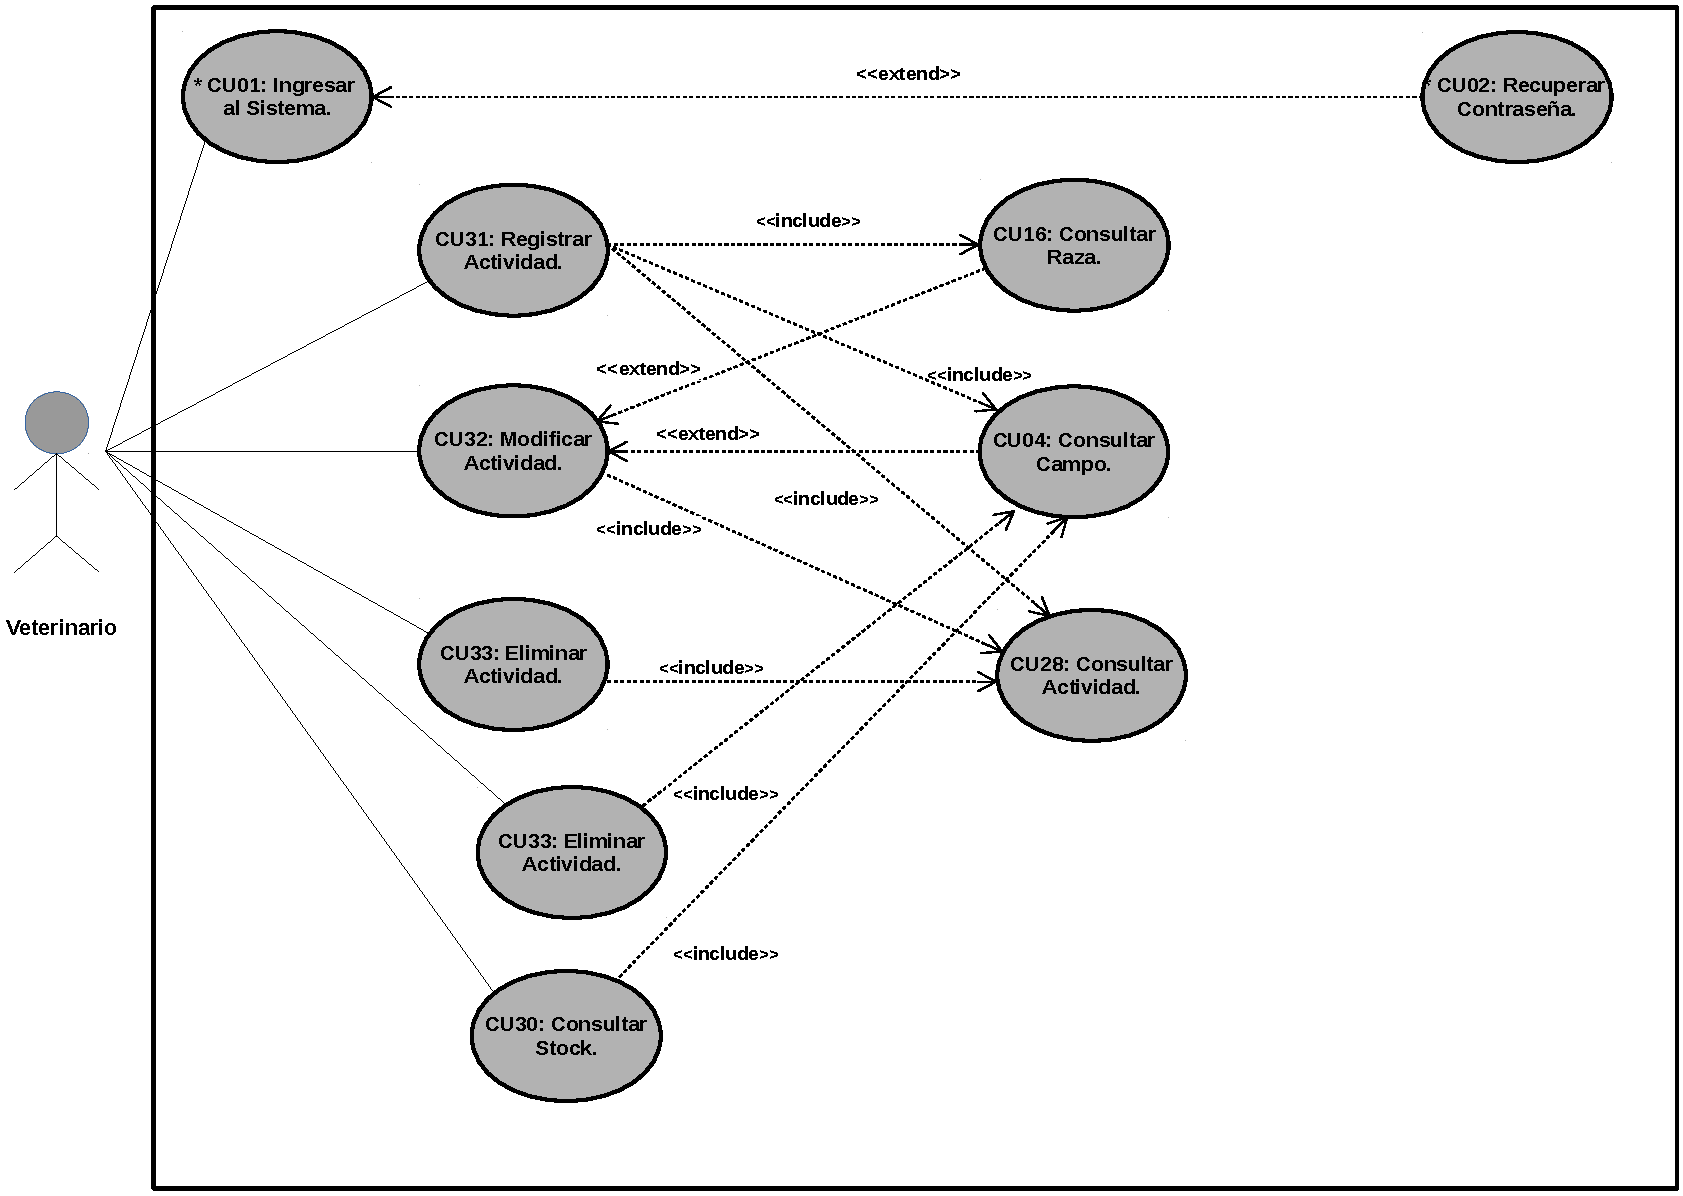
\includegraphics[scale=0.5]{figs/Diagrama_CU_Veterinario.pdf}}
\caption{Diagrama de Casos de Uso del Actor \textbf{Veterinario}.}
\label{Ap104}
\end{figure}

\newpage
\clearpage
\subsection{Fichas Textuales de Casos de Uso}\label{ApFCU}

\begin{figure}[tbhp]
\centerline{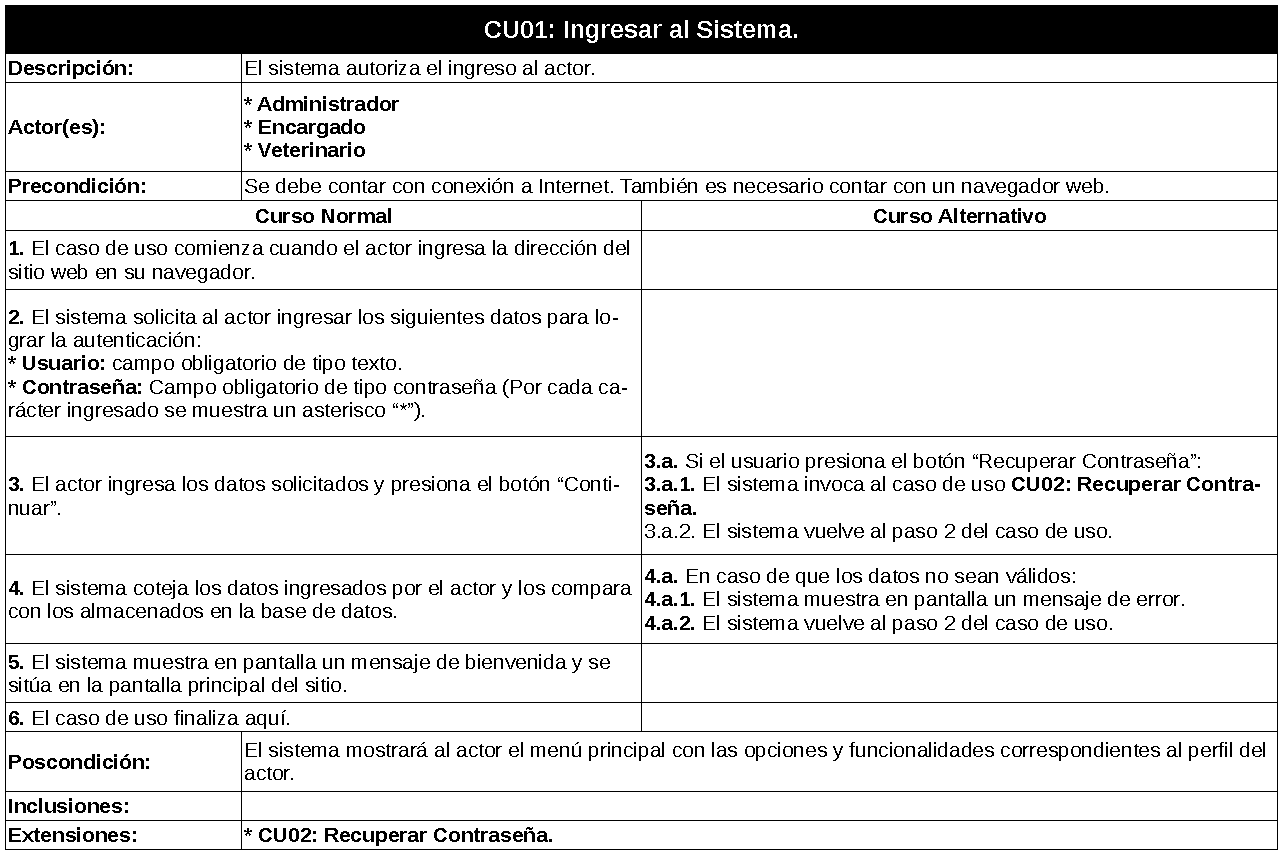
\includegraphics[scale=0.6]{Fichas_CU/pg_0001.pdf}}
\caption{CU01: Ingresar al Sistema.}
\label{Ap201}
\end{figure}

\begin{figure}[tbhp]
\centerline{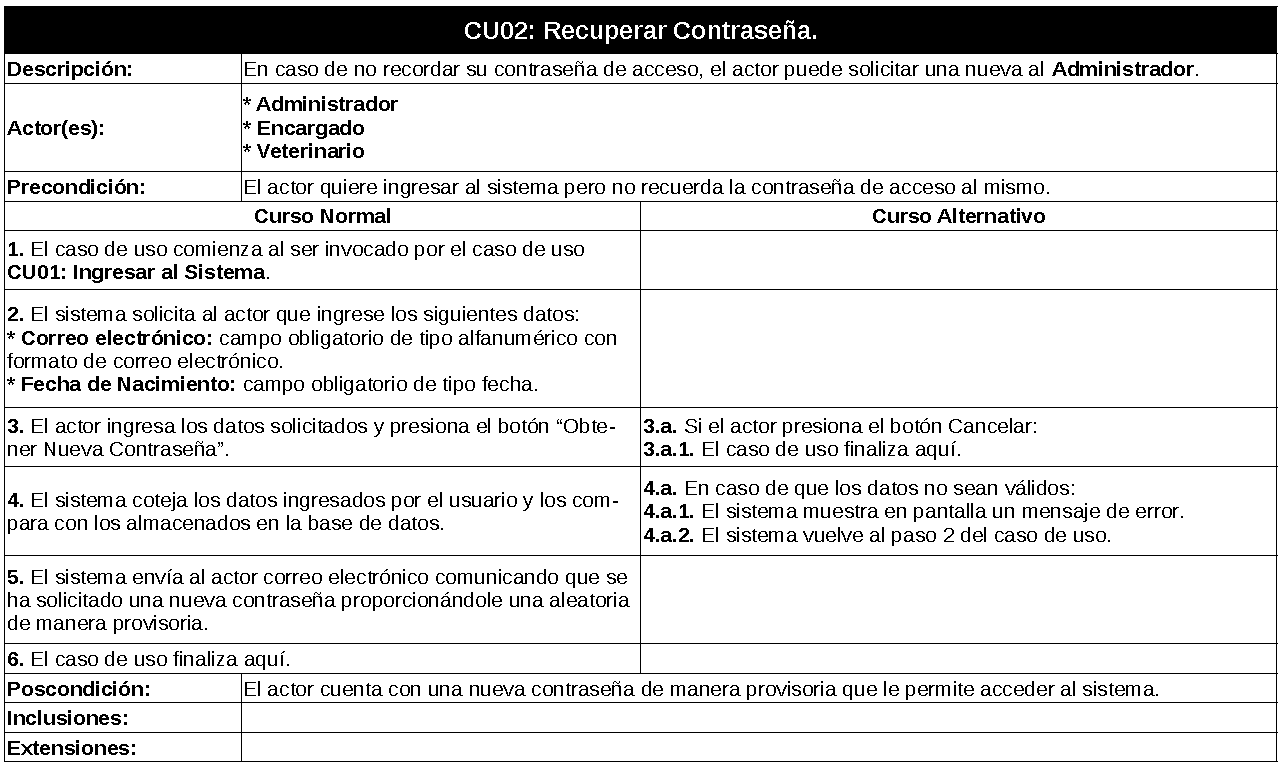
\includegraphics[scale=0.6]{Fichas_CU/pg_0002.pdf}}
\caption{CU02: Recuperar Contraseña.}
\label{Ap202}
\end{figure}

\begin{figure}[tbhp]
\centerline{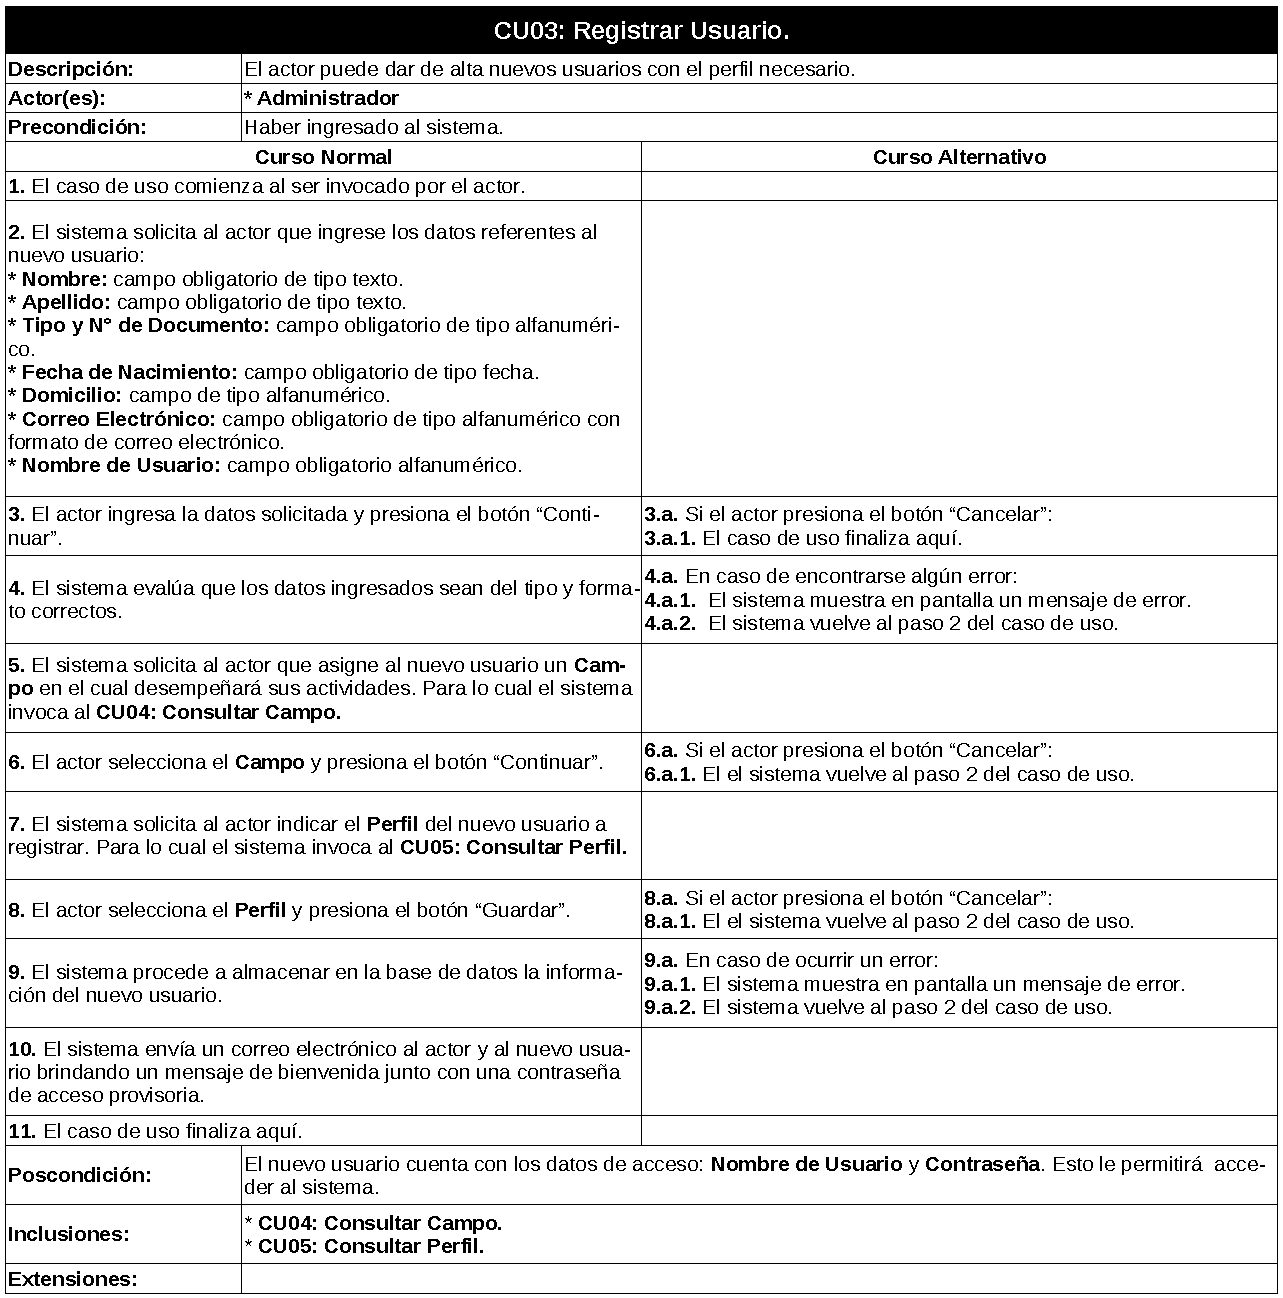
\includegraphics[scale=0.6]{Fichas_CU/pg_0003.pdf}}
\caption{CU03: Registrar Usuario.}
\label{Ap203}
\end{figure}

\begin{figure}[tbhp]
\centerline{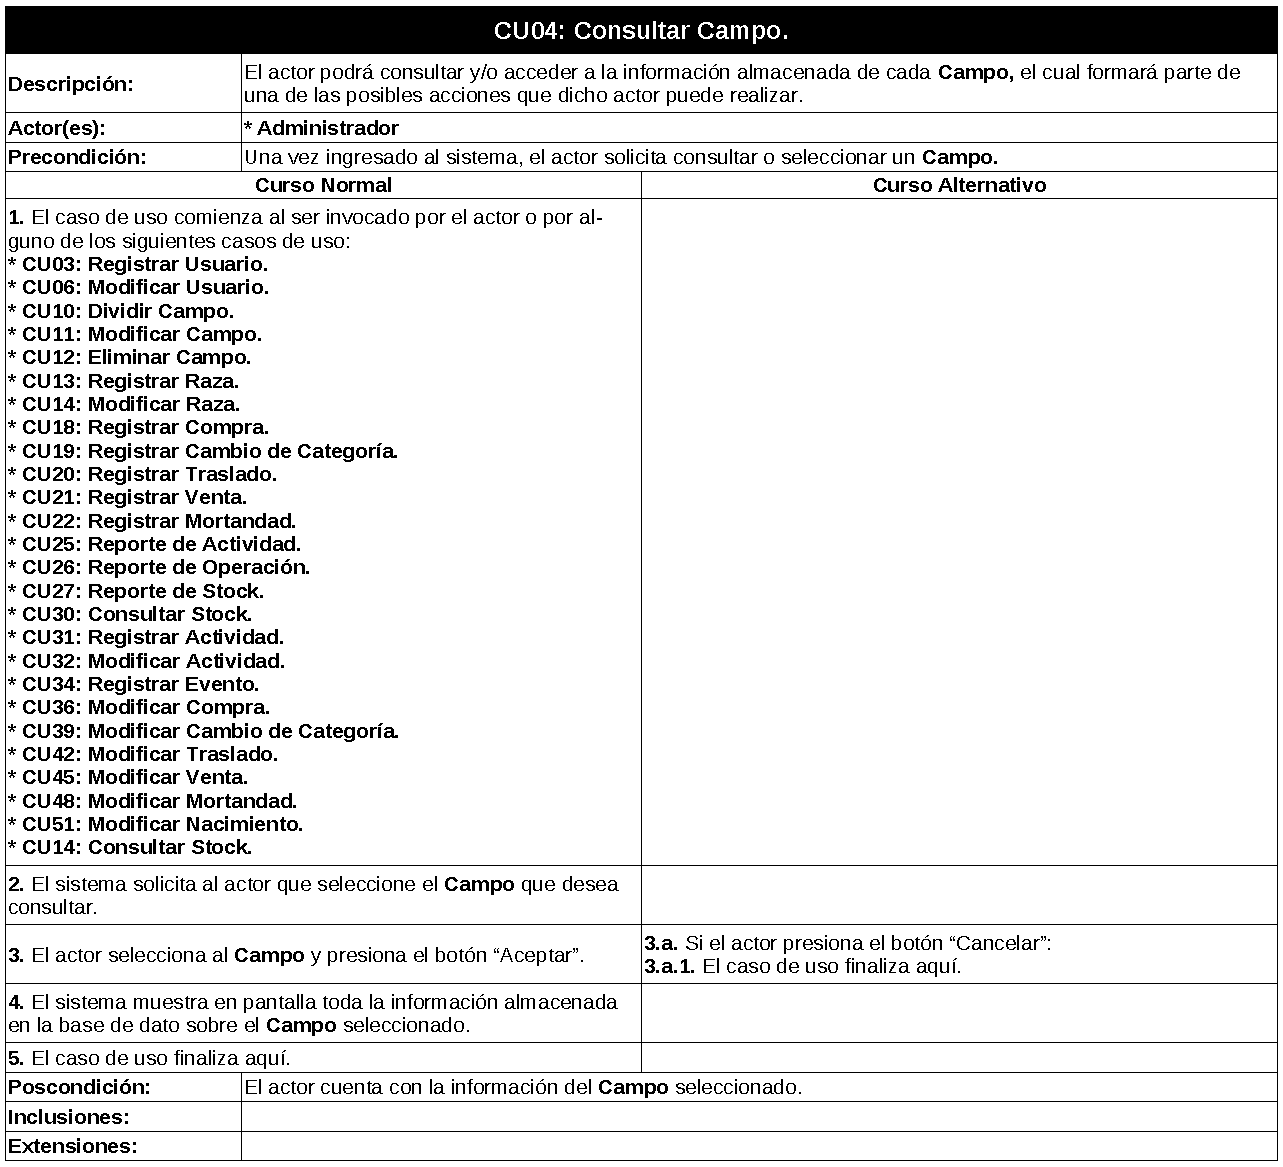
\includegraphics[scale=0.6]{Fichas_CU/pg_0004.pdf}}
\caption{CU04: Consultar Campo.}
\label{Ap204}
\end{figure}

\begin{figure}[tbhp]
\centerline{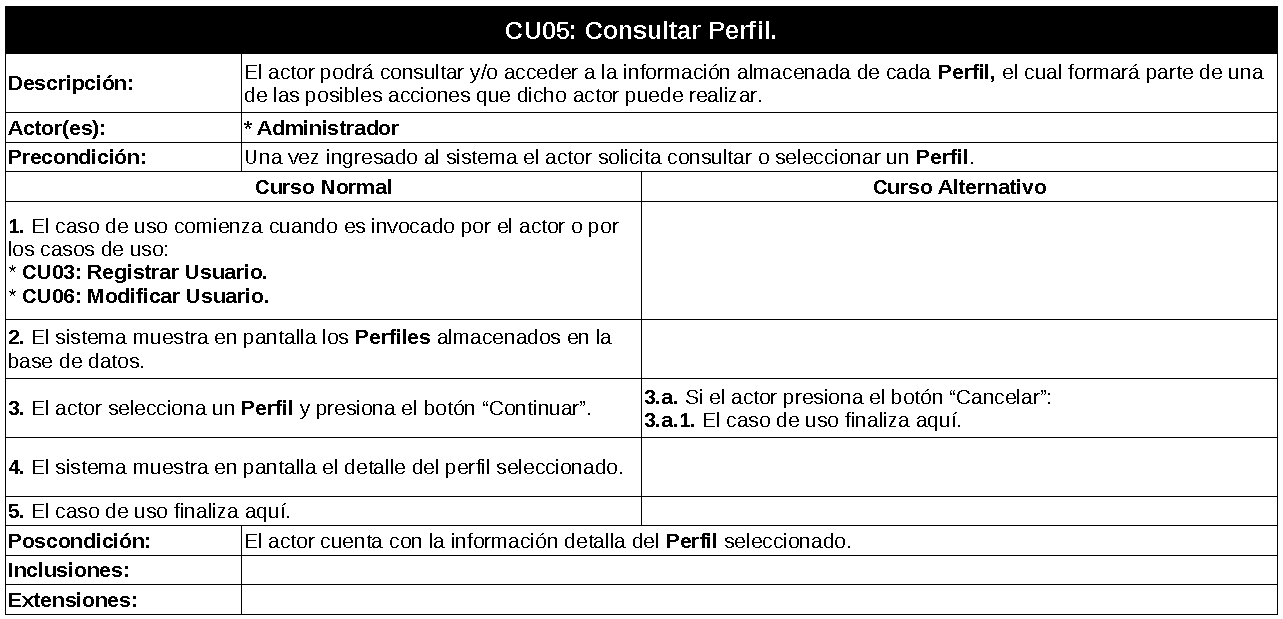
\includegraphics[scale=0.6]{Fichas_CU/pg_0005.pdf}}
\caption{CU05: Consultar Perfil.}
\label{Ap205}
\end{figure}

\begin{figure}[tbhp]
\centerline{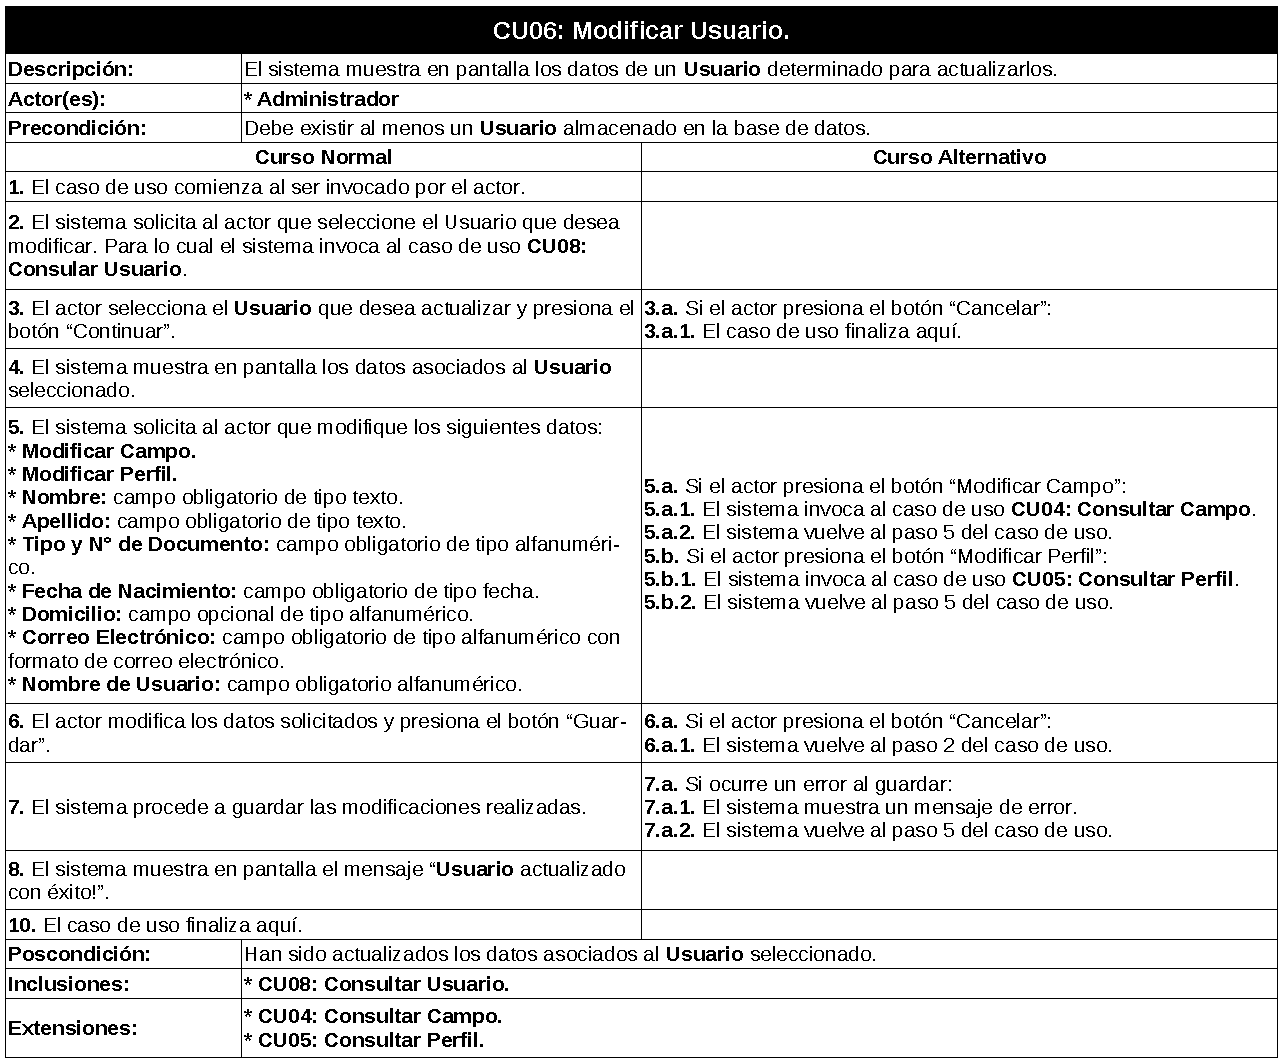
\includegraphics[scale=0.6]{Fichas_CU/pg_0006.pdf}}
\caption{CU06: Modificar Usuario.}
\label{Ap206}
\end{figure}

\begin{figure}[tbhp]
\centerline{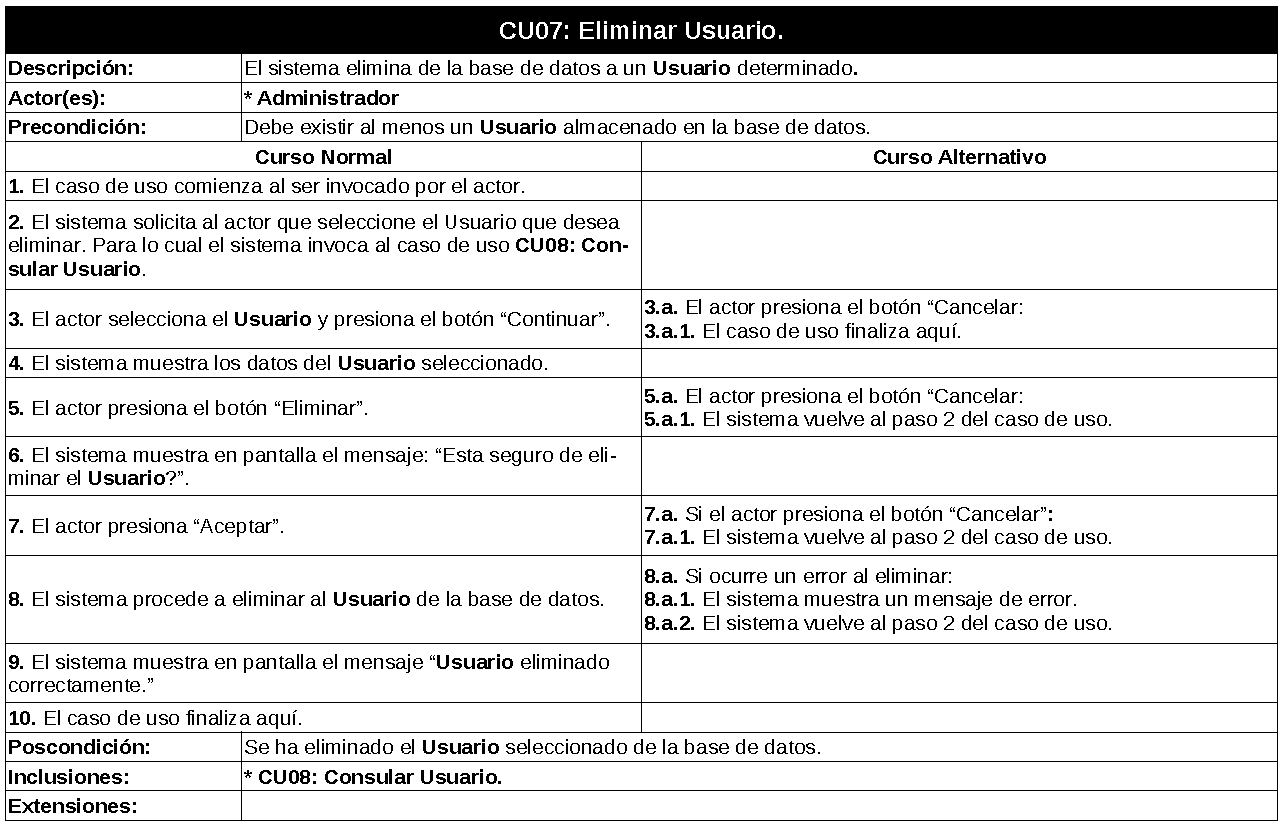
\includegraphics[scale=0.6]{Fichas_CU/pg_0007.pdf}}
\caption{CU07: Eliminar Usuario.}
\label{Ap207}
\end{figure}

\begin{figure}[tbhp]
\centerline{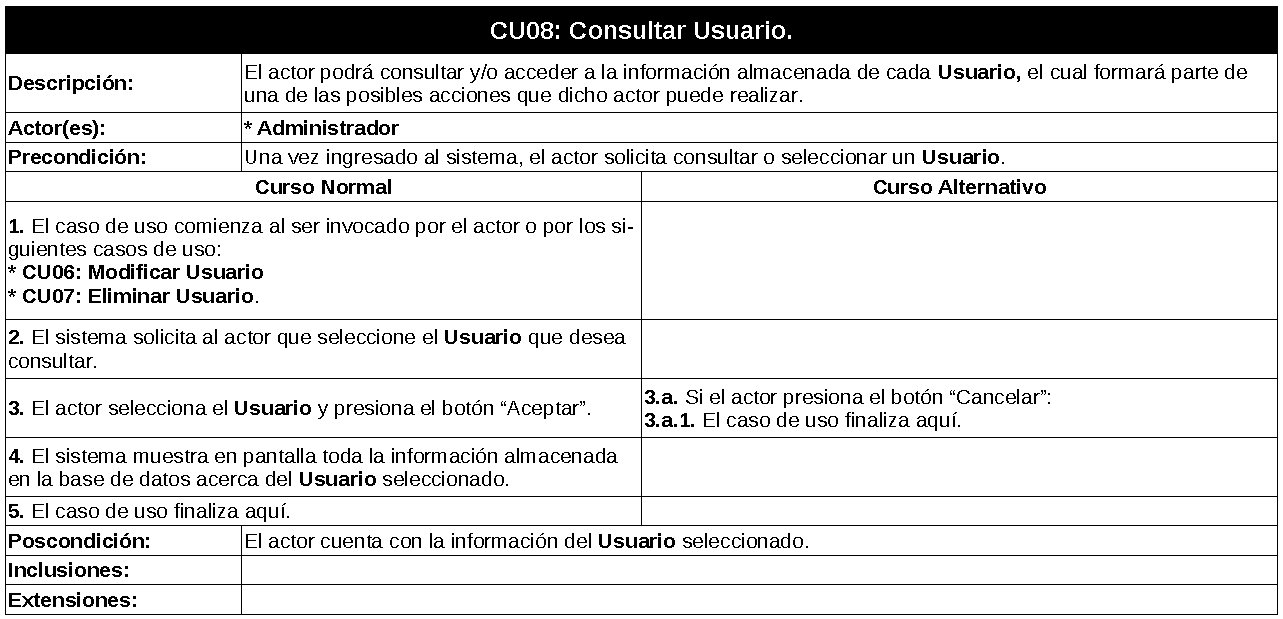
\includegraphics[scale=0.6]{Fichas_CU/pg_0008.pdf}}
\caption{CU08: Consultar Usuario.}
\label{Ap208}
\end{figure}

\begin{figure}[tbhp]
\centerline{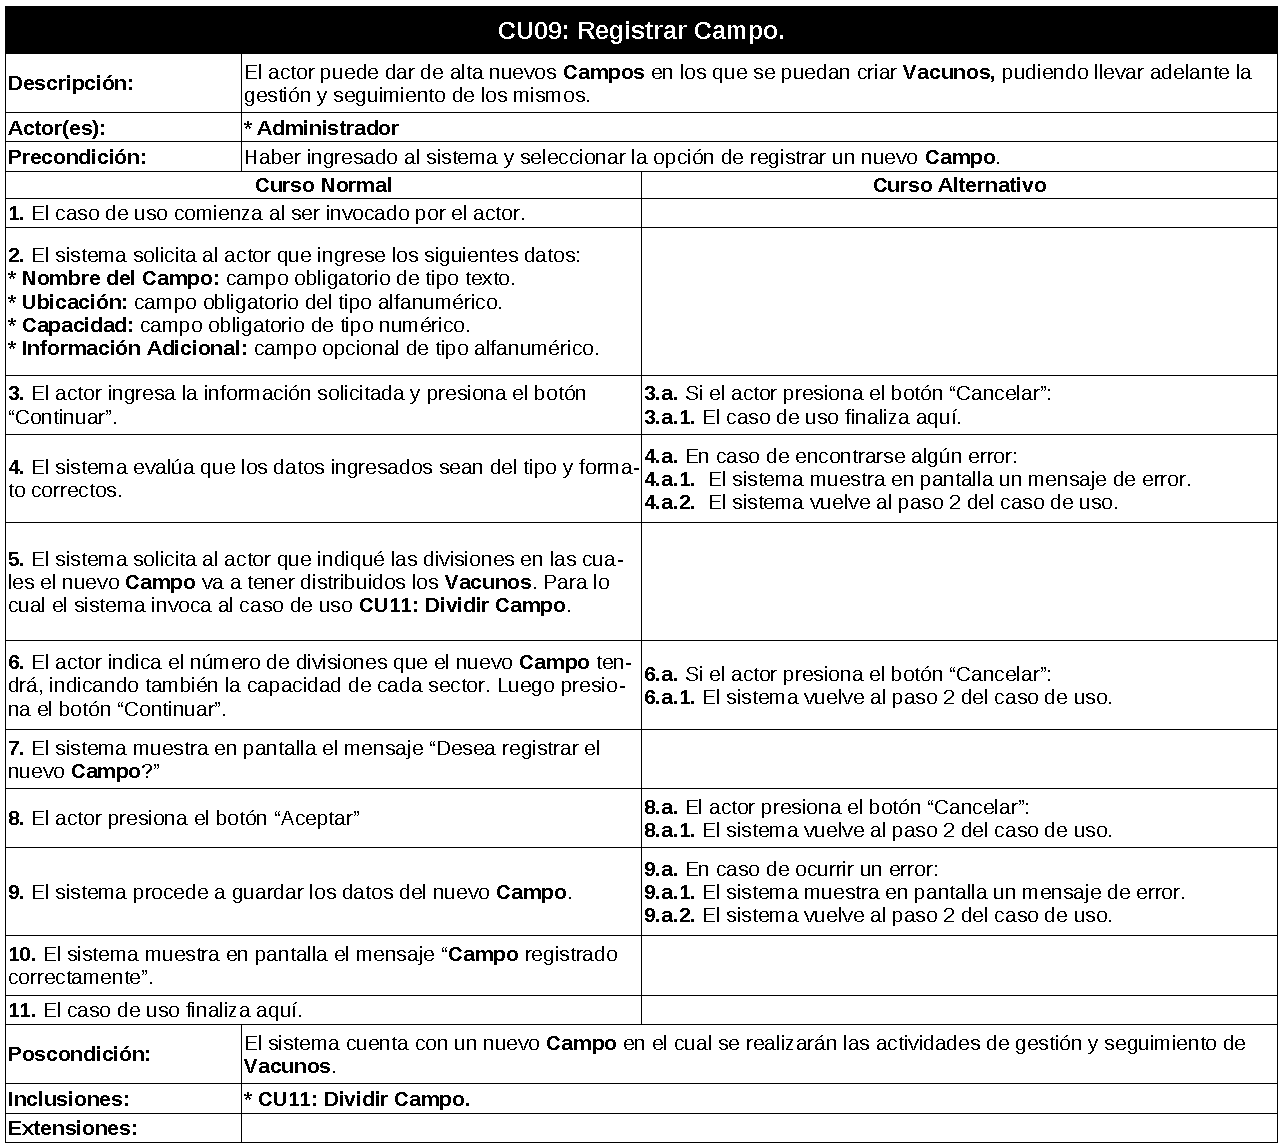
\includegraphics[scale=0.6]{Fichas_CU/pg_0009.pdf}}
\caption{CU09: Registrar Campo.}
\label{Ap209}
\end{figure}

\begin{figure}[tbhp]
\centerline{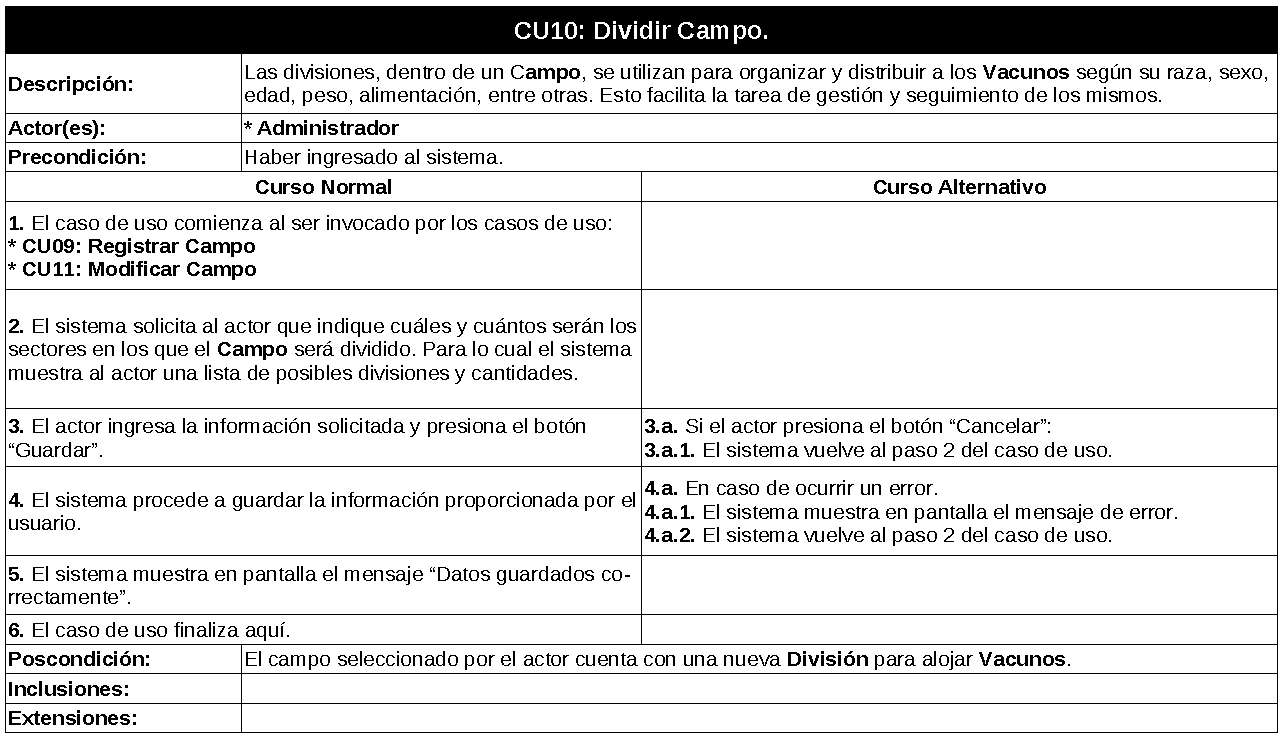
\includegraphics[scale=0.6]{Fichas_CU/pg_0010.pdf}}
\caption{CU10: Dividir Campo.}
\label{Ap210}
\end{figure}

\begin{figure}[tbhp]
\centerline{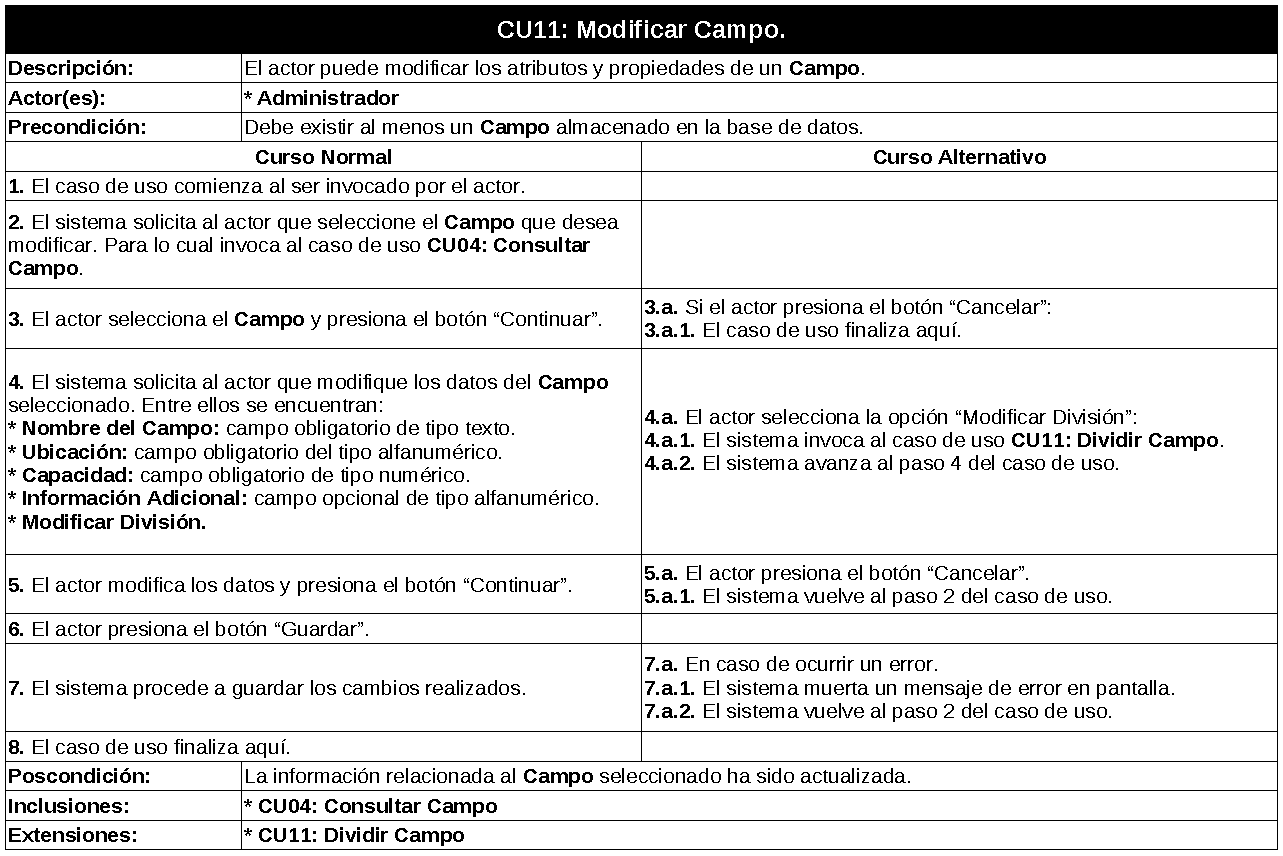
\includegraphics[scale=0.6]{Fichas_CU/pg_0011.pdf}}
\caption{CU11: Modificar Campo.}
\label{Ap211}
\end{figure}

\begin{figure}[tbhp]
\centerline{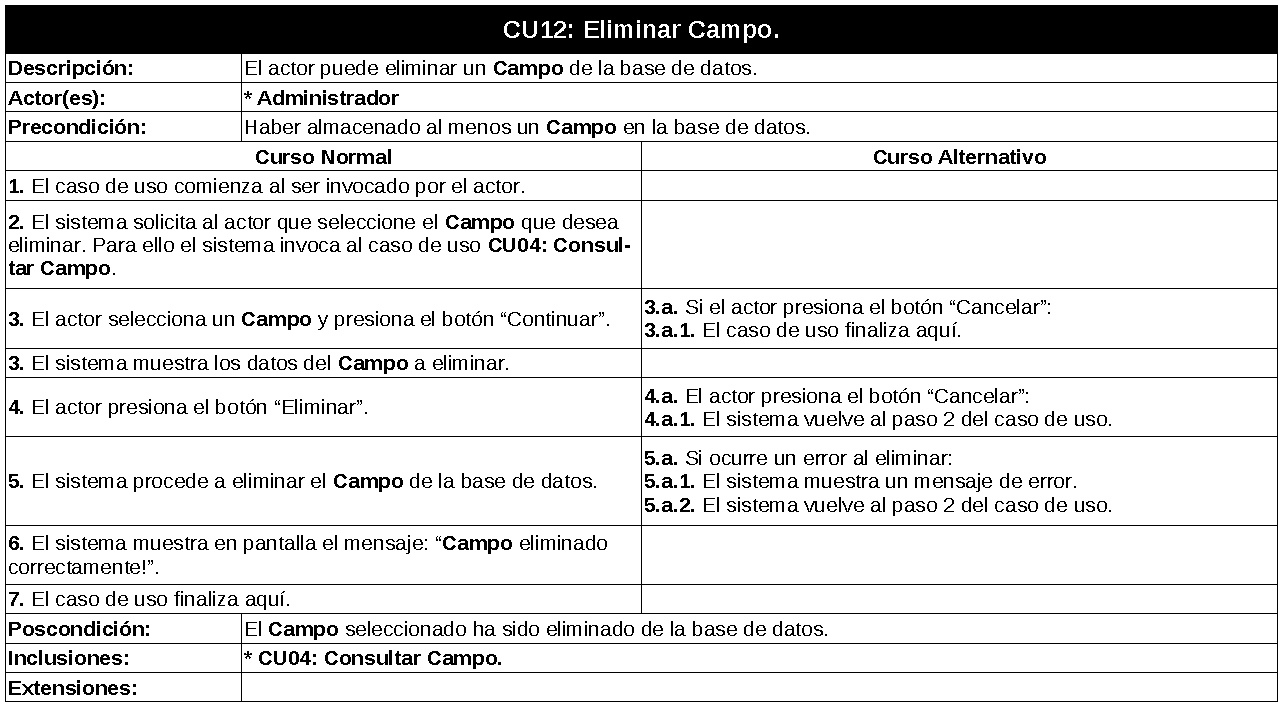
\includegraphics[scale=0.6]{Fichas_CU/pg_0012.pdf}}
\caption{CU12: Eliminar Campo.}
\label{Ap212}
\end{figure}

\begin{figure}[tbhp]
\centerline{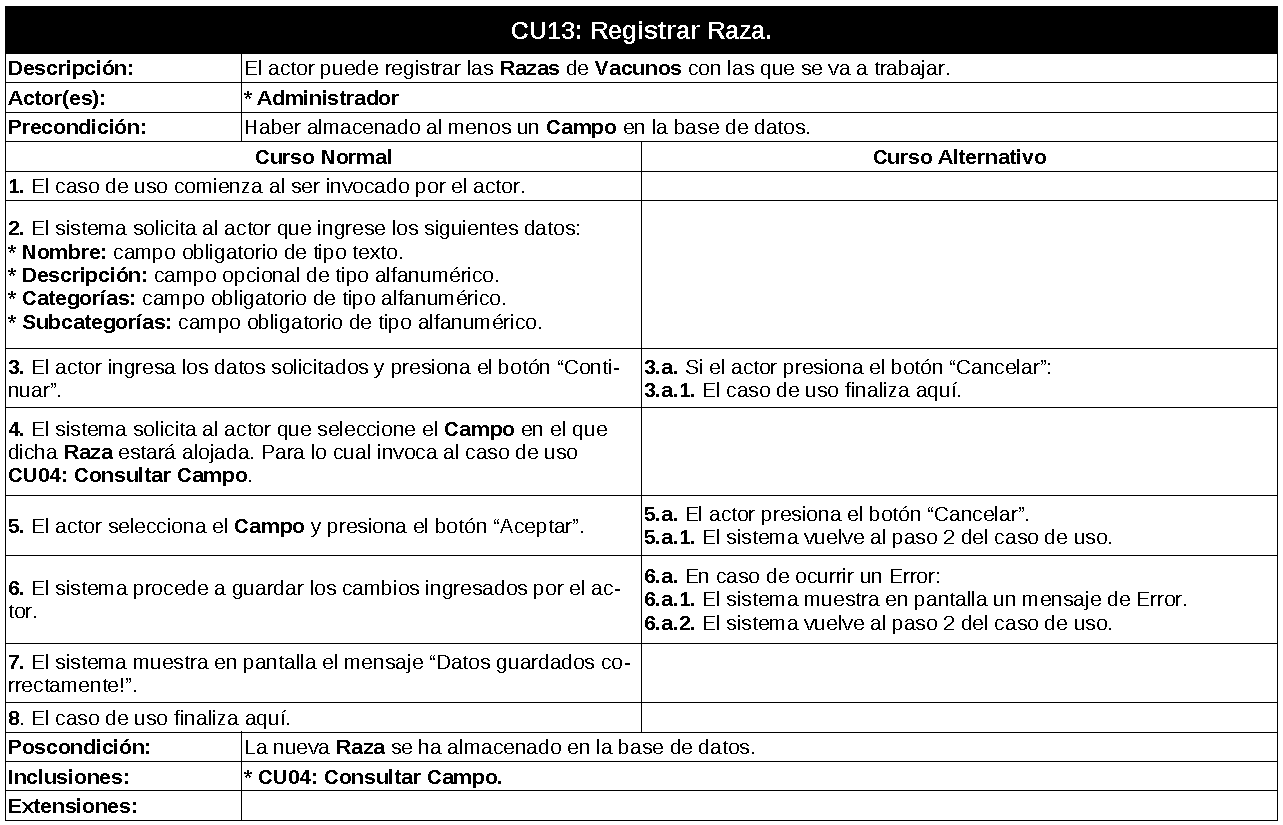
\includegraphics[scale=0.6]{Fichas_CU/pg_0013.pdf}}
\caption{CU13: Registrar Raza.}
\label{Ap213}
\end{figure}

\begin{figure}[tbhp]
\centerline{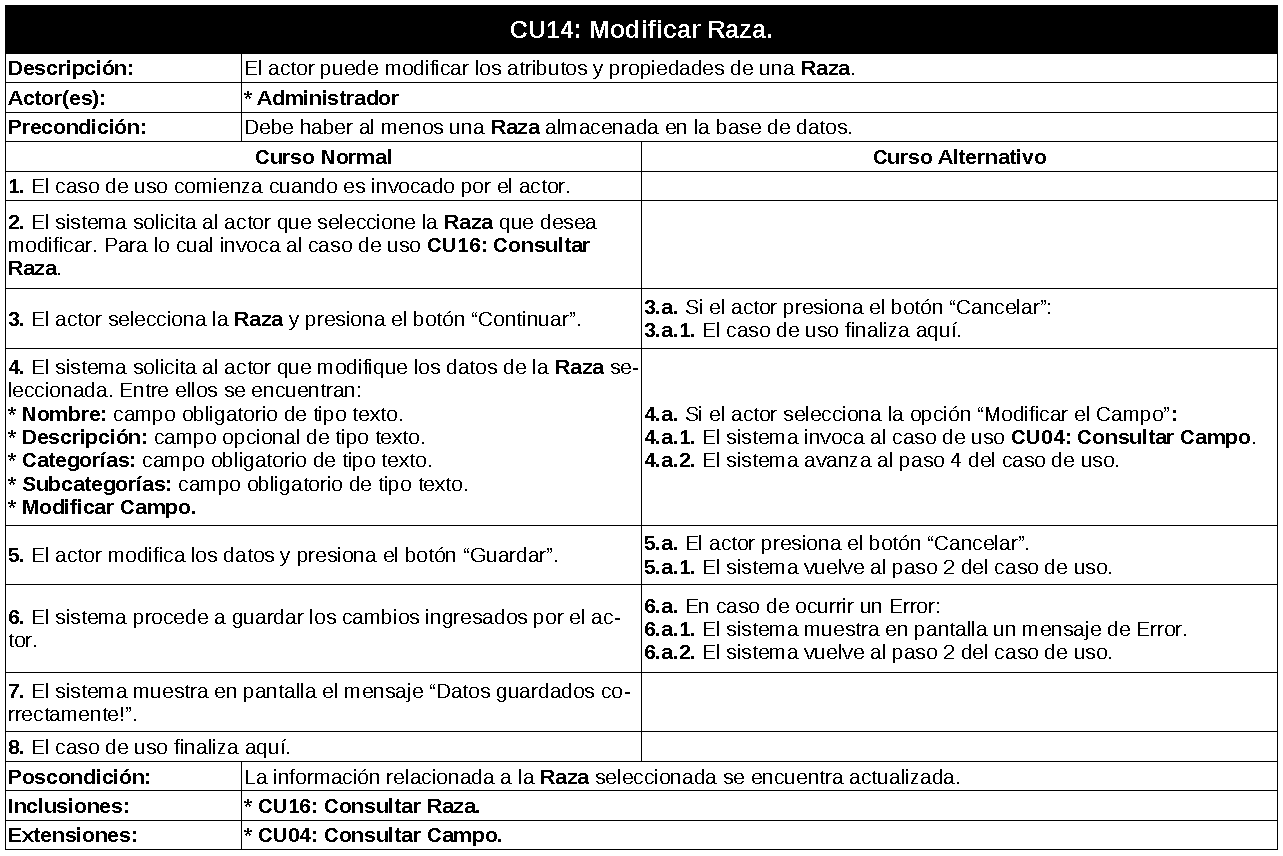
\includegraphics[scale=0.6]{Fichas_CU/pg_0014.pdf}}
\caption{CU14: Modificar Raza.}
\label{Ap214}
\end{figure}

\begin{figure}[tbhp]
\centerline{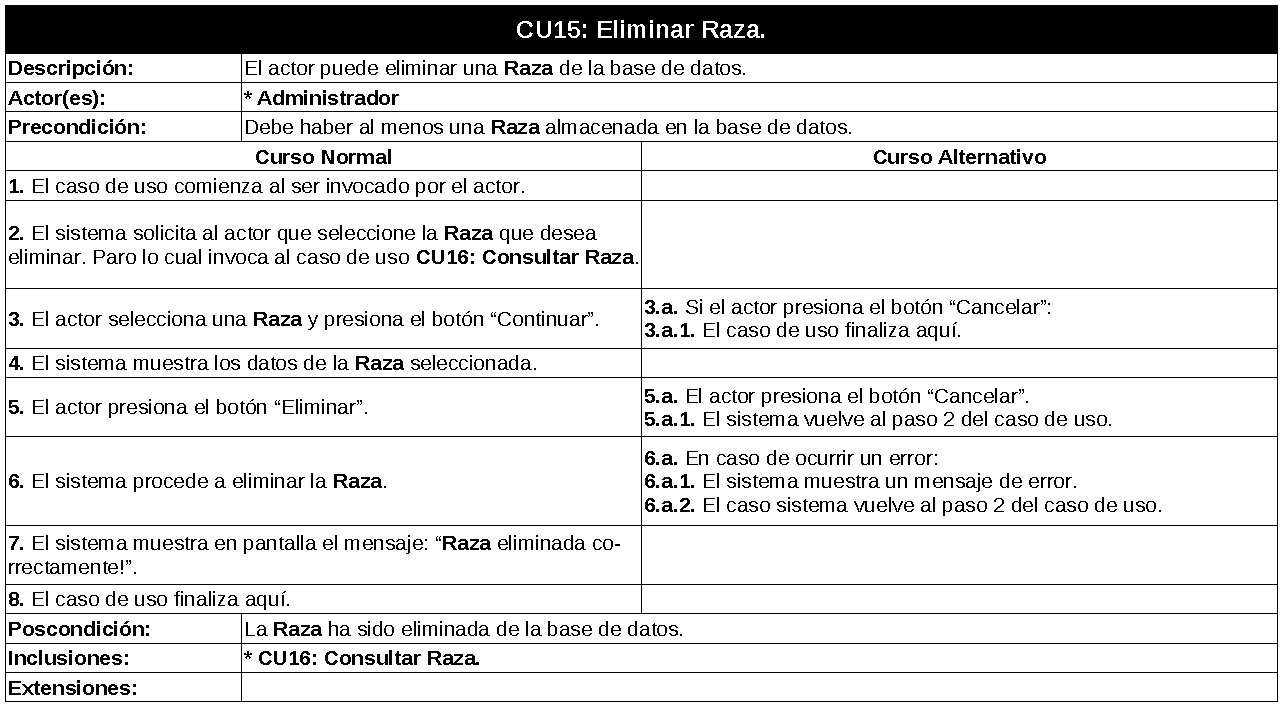
\includegraphics[scale=0.6]{Fichas_CU/pg_0015.pdf}}
\caption{CU15: Eliminar Raza.}
\label{Ap215}
\end{figure}

\begin{figure}[tbhp]
\centerline{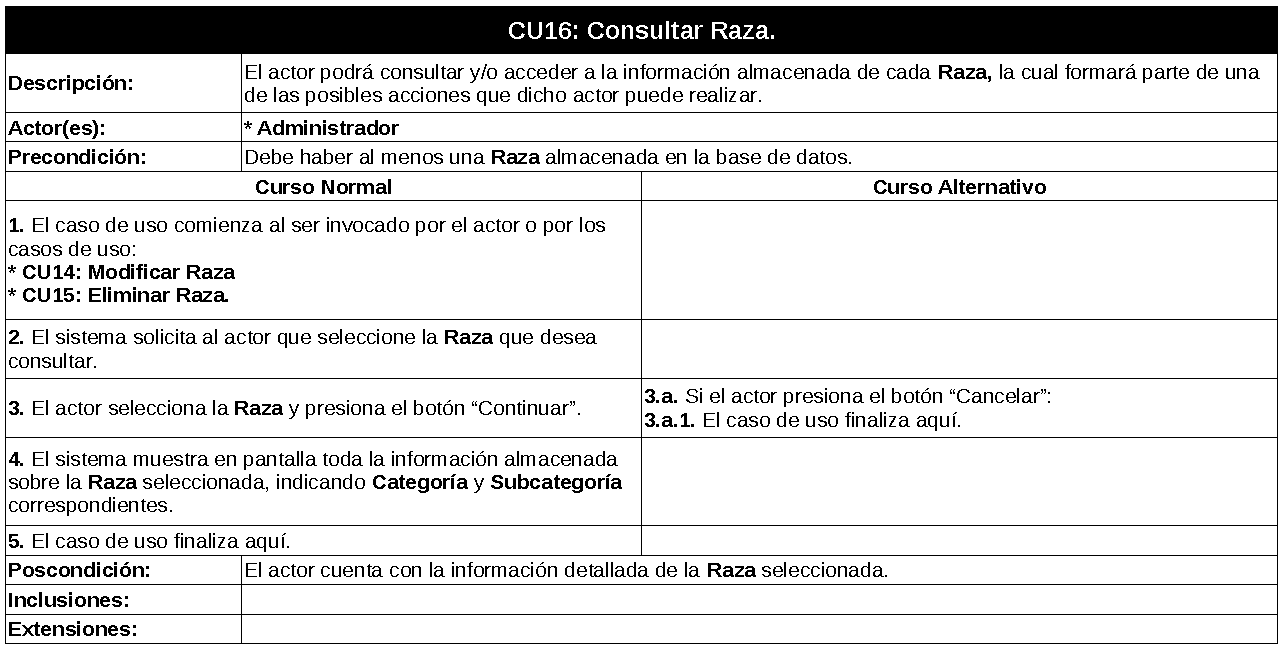
\includegraphics[scale=0.6]{Fichas_CU/pg_0016.pdf}}
\caption{CU16: Consultar Raza.}
\label{Ap216}
\end{figure}

\begin{figure}[tbhp]
\centerline{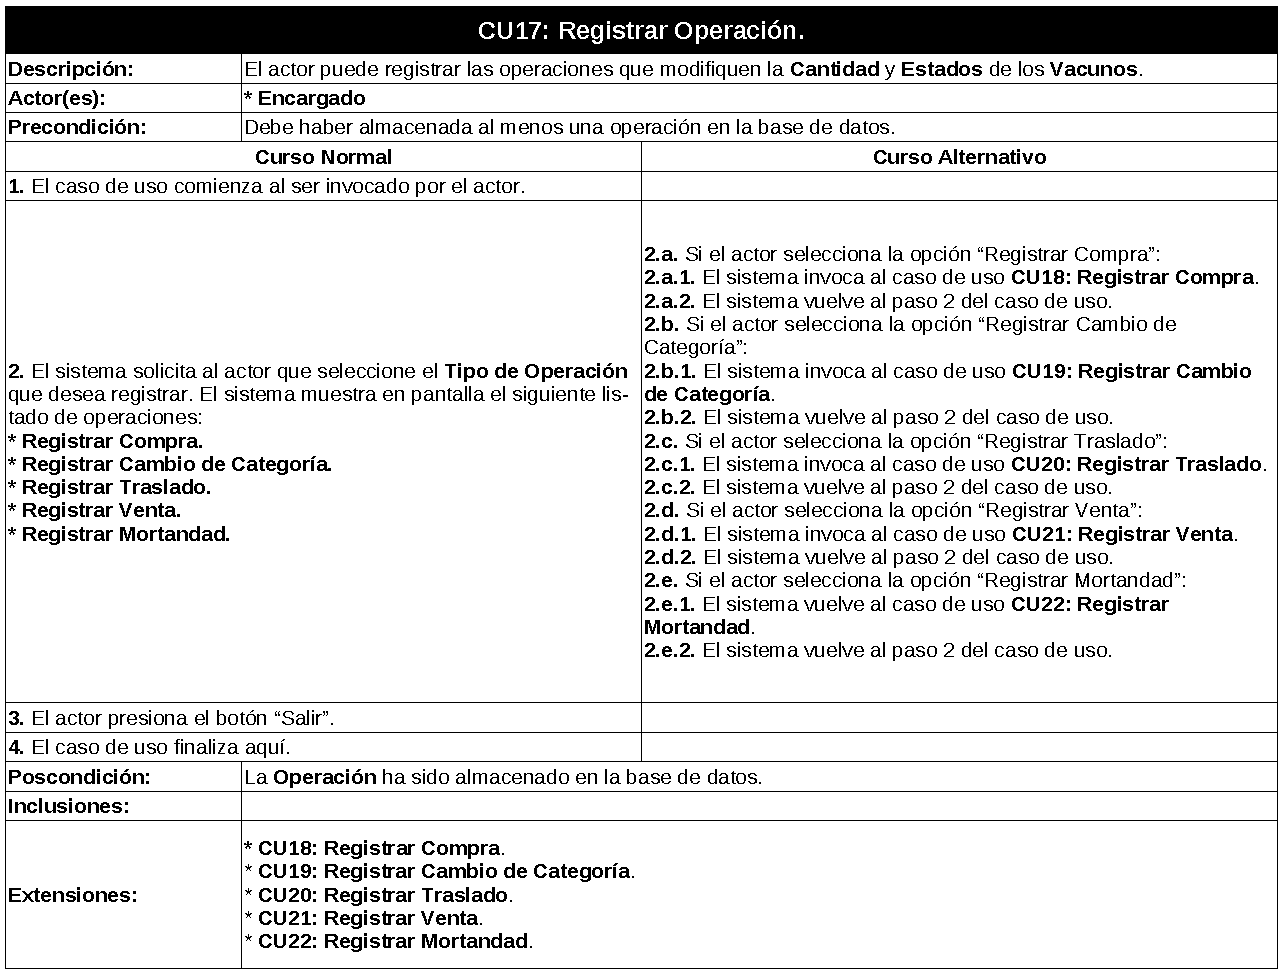
\includegraphics[scale=0.6]{Fichas_CU/pg_0017.pdf}}
\caption{CU17: Registrar Operación.}
\label{Ap217}
\end{figure}

\begin{figure}[tbhp]
\centerline{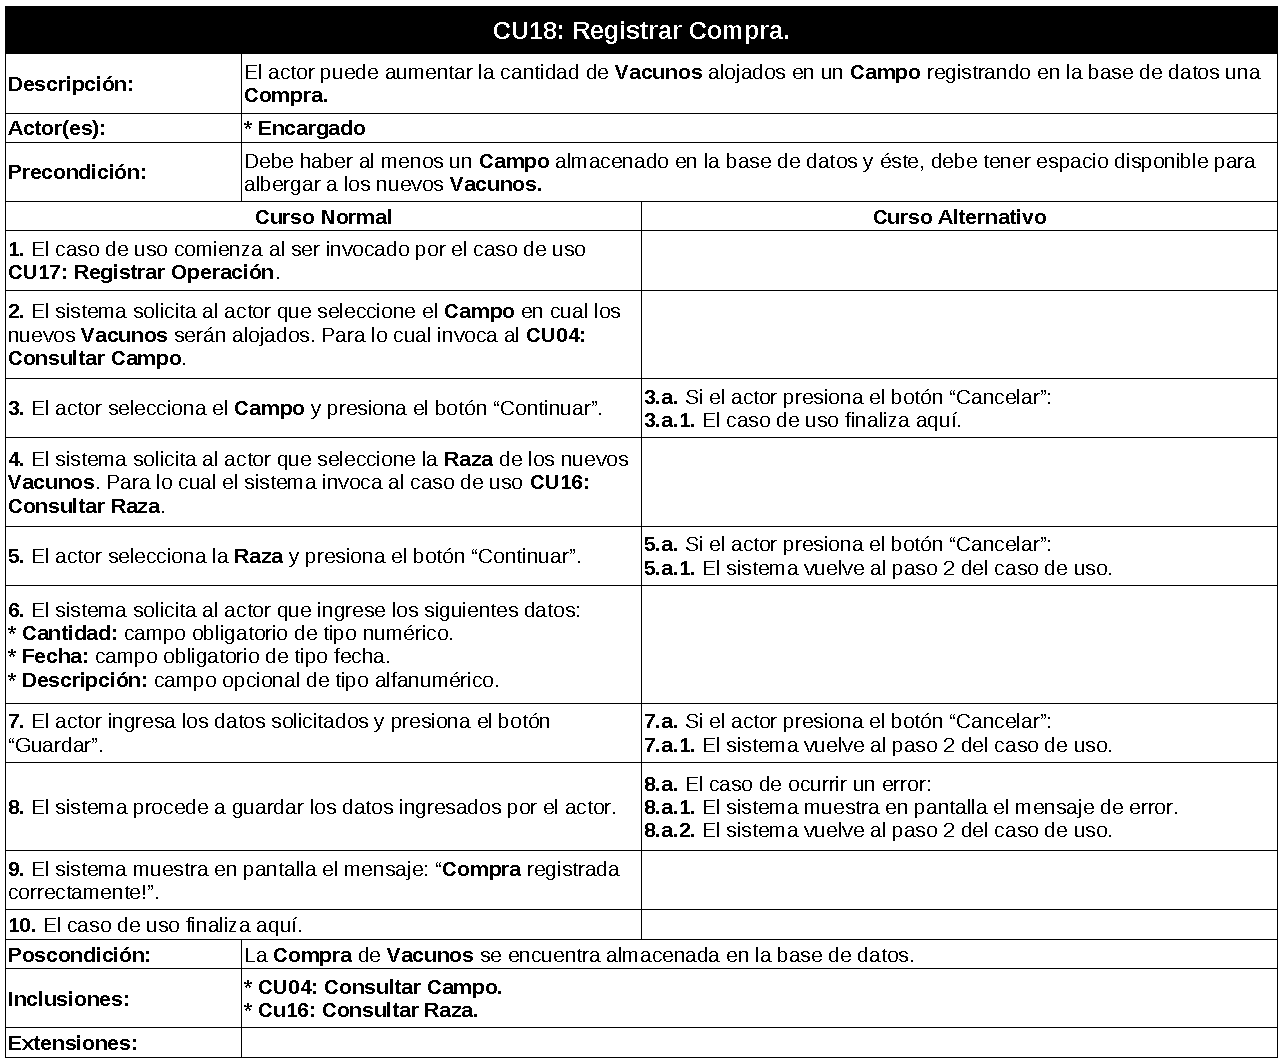
\includegraphics[scale=0.6]{Fichas_CU/pg_0018.pdf}}
\caption{CU18: Registrar Compra.}
\label{Ap218}
\end{figure}

\begin{figure}[tbhp]
\centerline{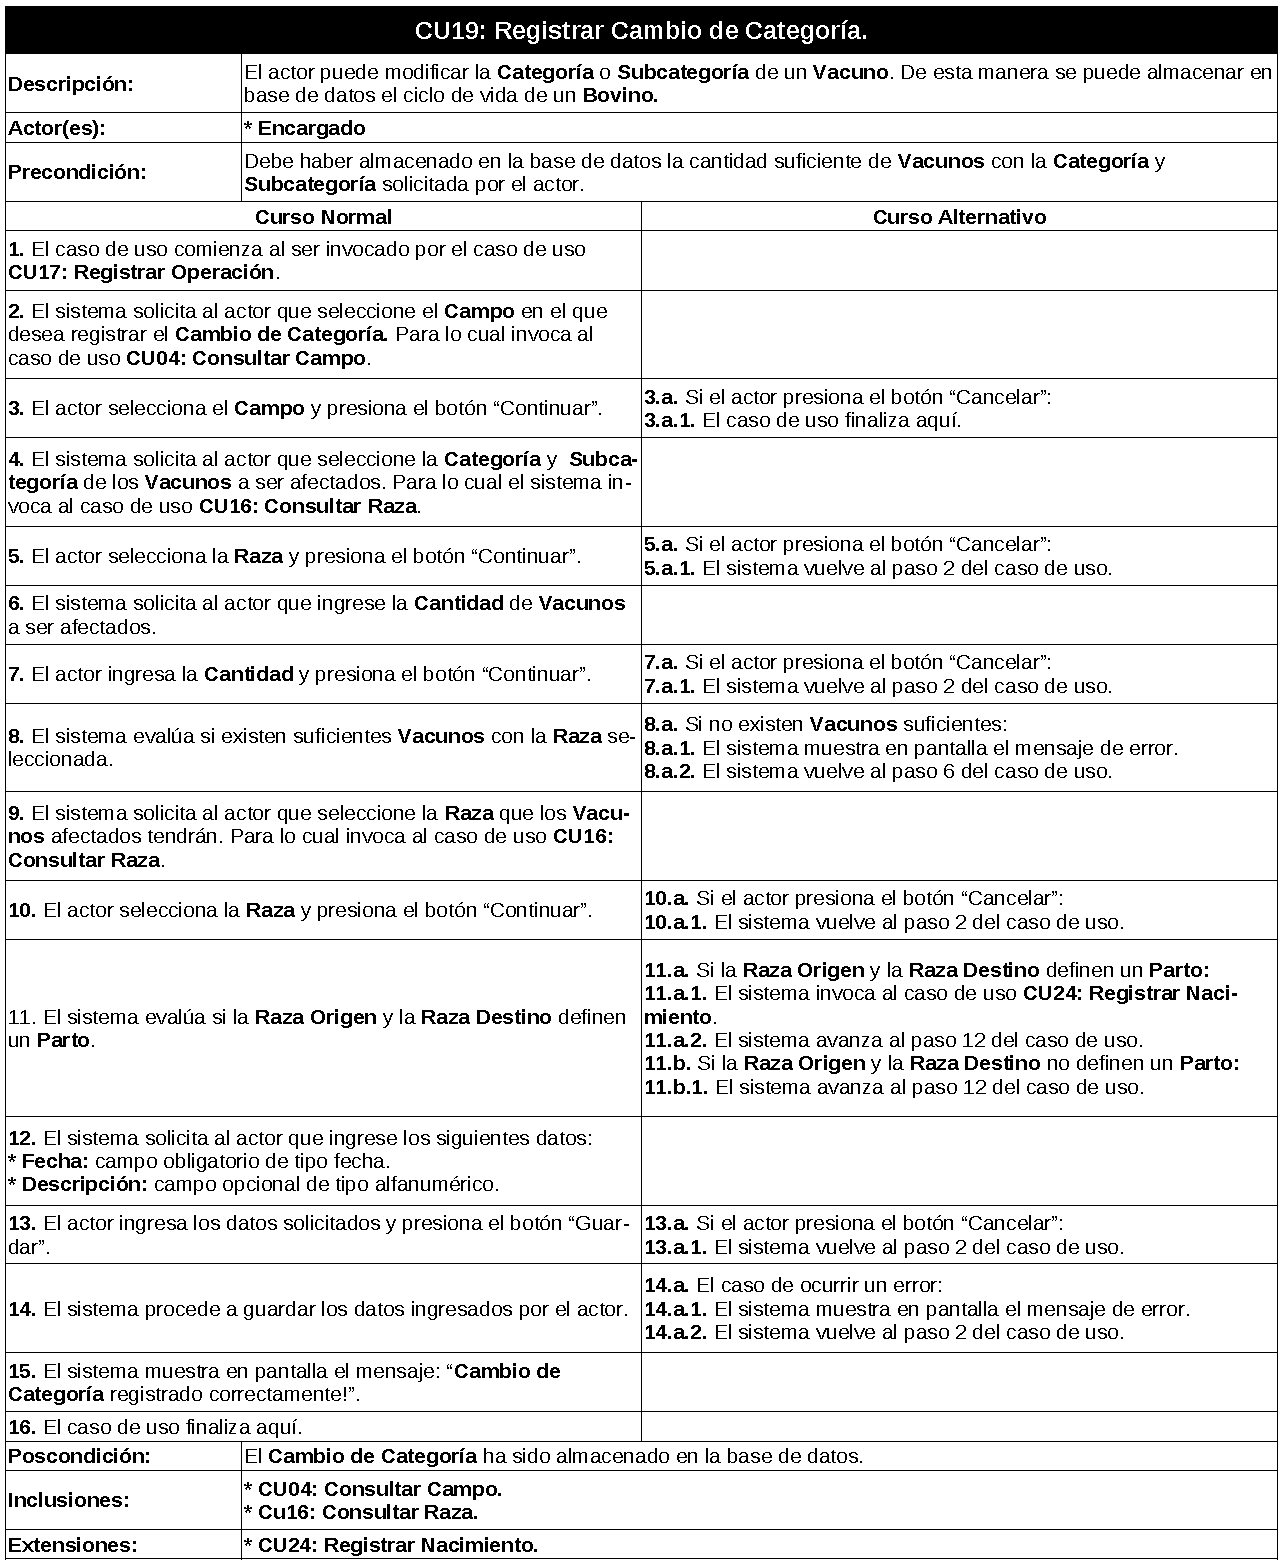
\includegraphics[scale=0.6]{Fichas_CU/pg_0019.pdf}}
\caption{CU19: Registrar Cambio de Categoría.}
\label{Ap219}
\end{figure}

\begin{figure}[tbhp]
\centerline{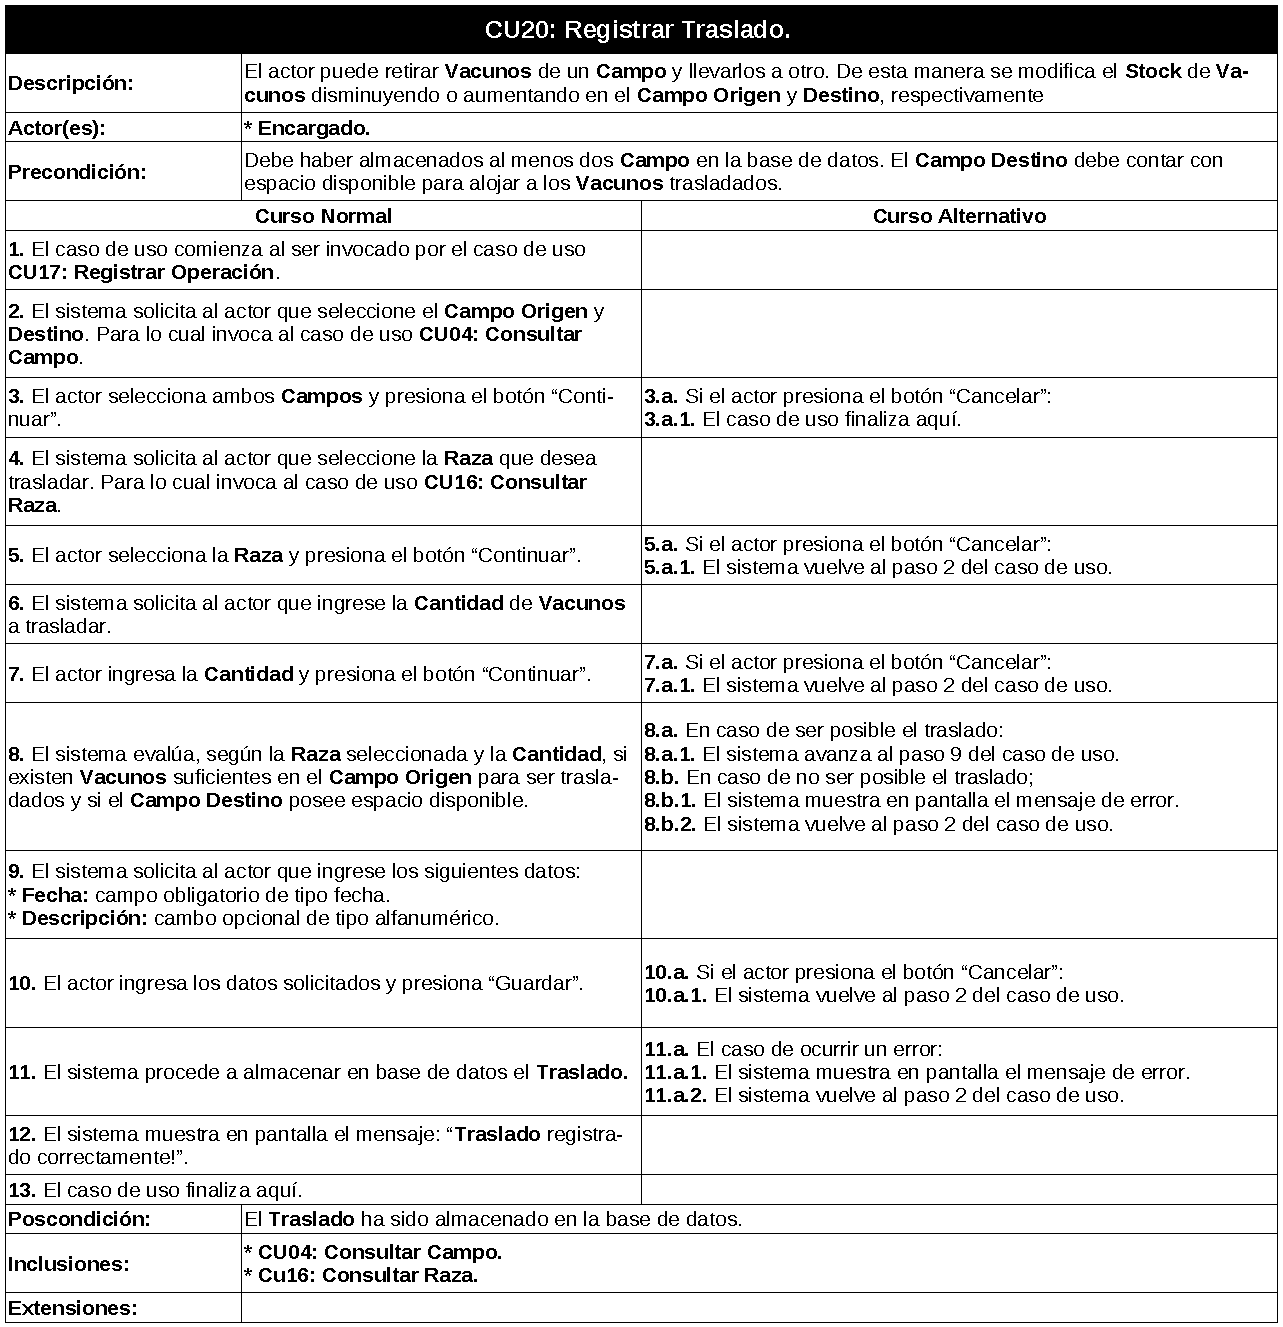
\includegraphics[scale=0.6]{Fichas_CU/pg_0020.pdf}}
\caption{CU20: Registrar Traslado.}
\label{Ap220}
\end{figure}

\begin{figure}[tbhp]
\centerline{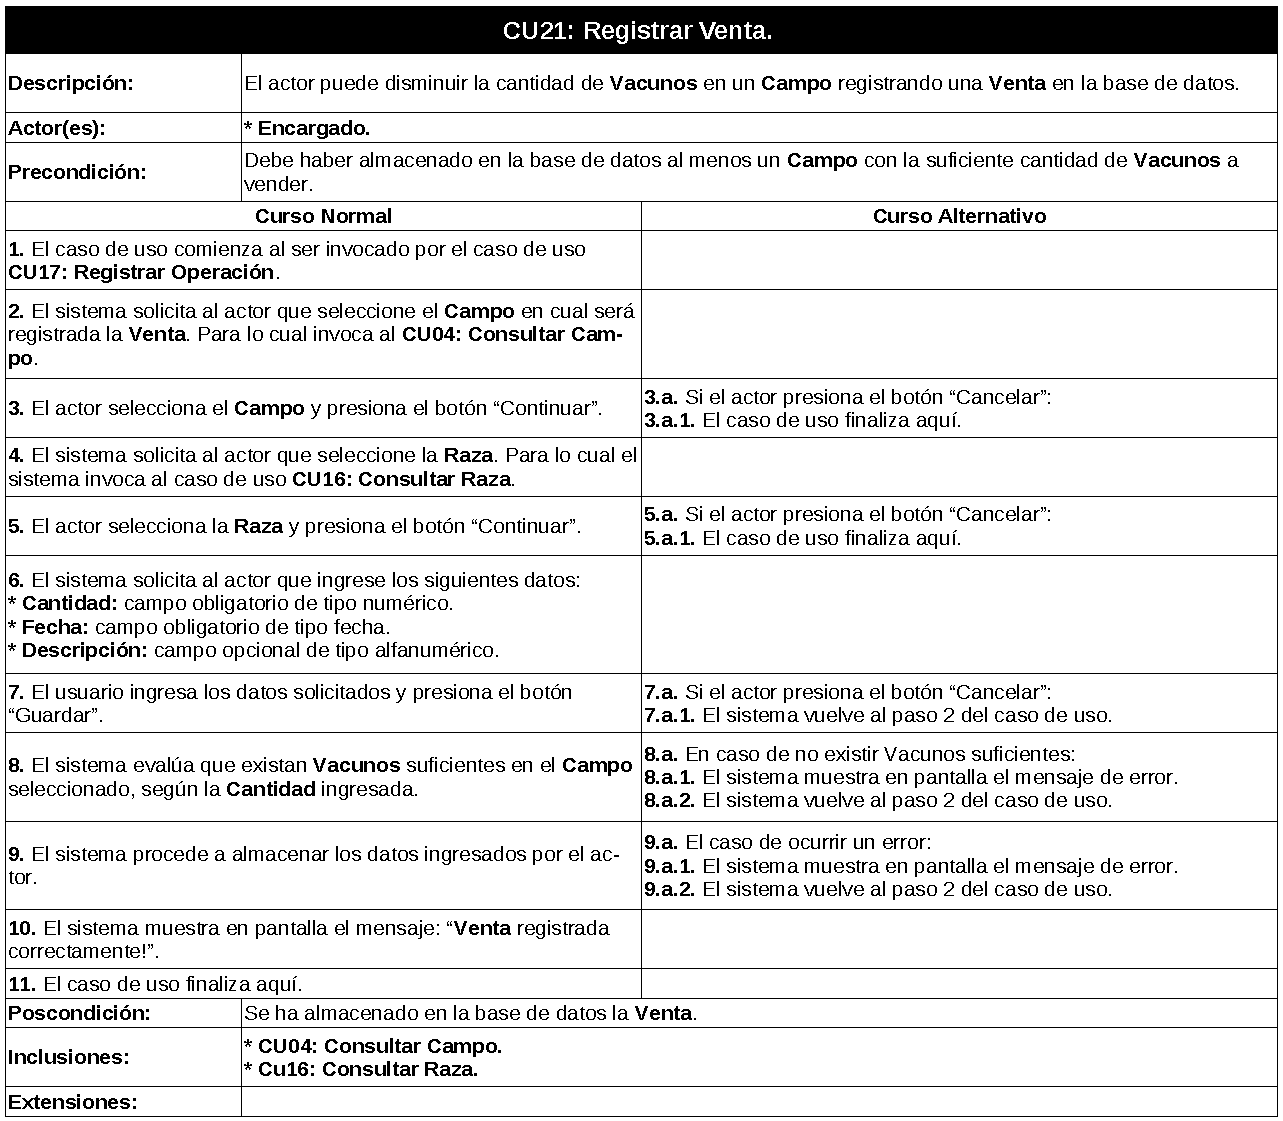
\includegraphics[scale=0.6]{Fichas_CU/pg_0021.pdf}}
\caption{CU21: Registrar Venta.}
\label{Ap221}
\end{figure}

\begin{figure}[tbhp]
\centerline{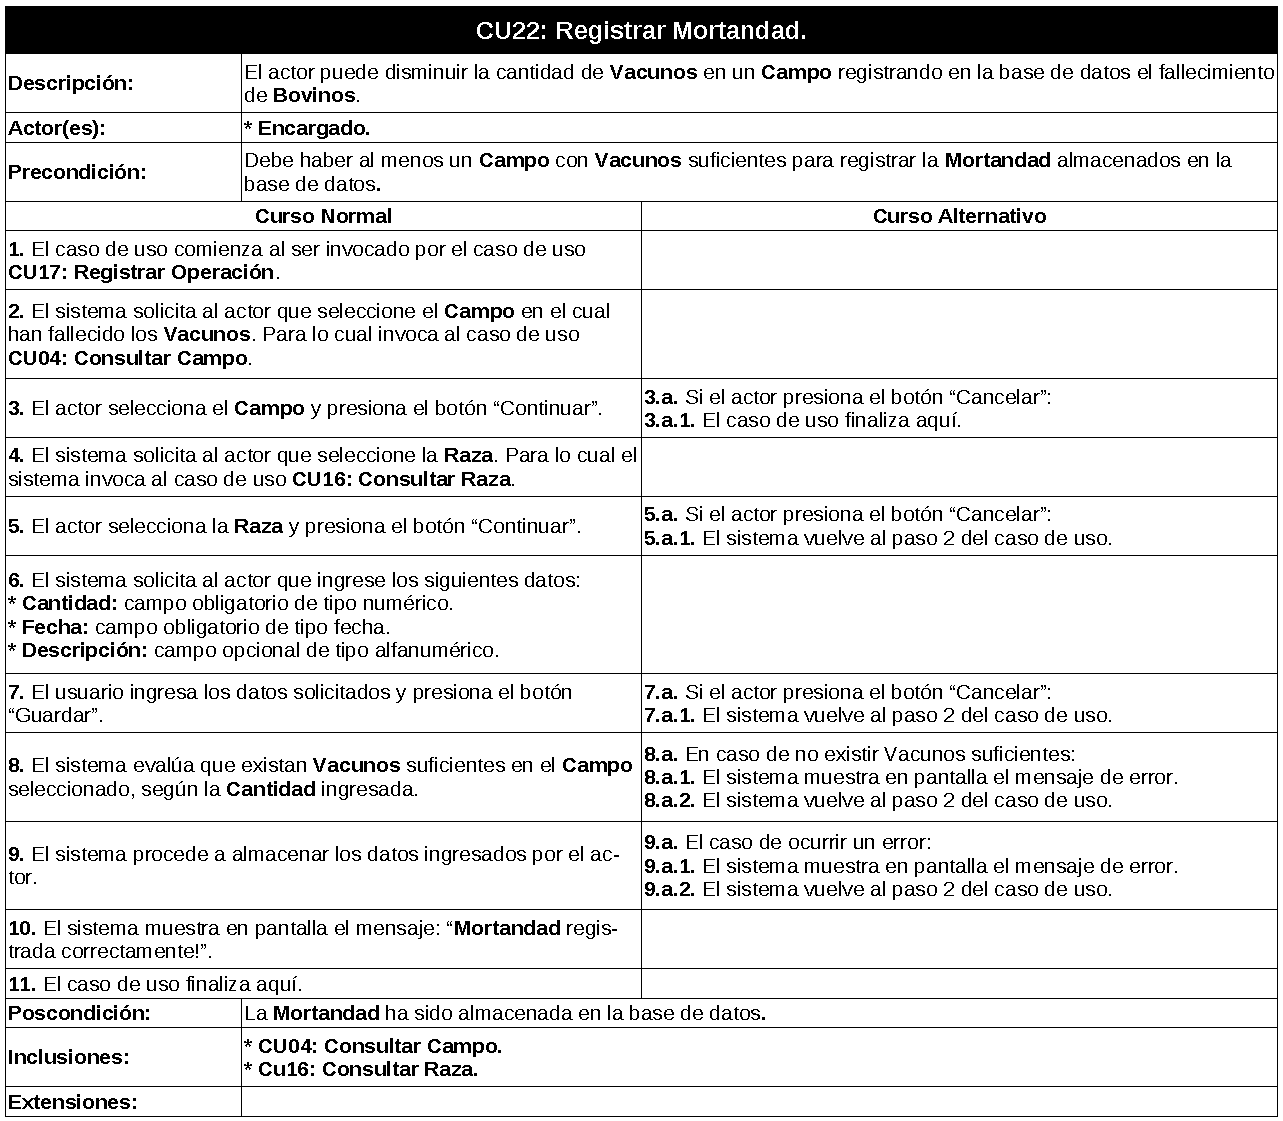
\includegraphics[scale=0.6]{Fichas_CU/pg_0022.pdf}}
\caption{CU22: Registrar Mortandad.}
\label{Ap222}
\end{figure}

\begin{figure}[tbhp]
\centerline{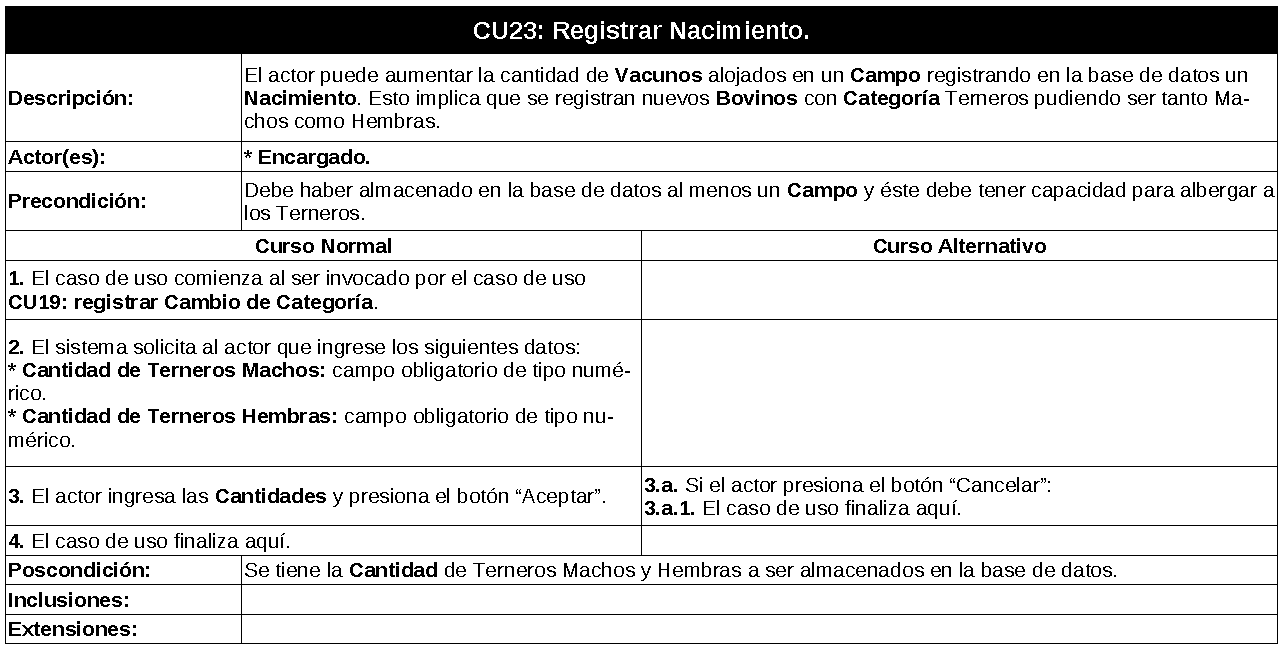
\includegraphics[scale=0.6]{Fichas_CU/pg_0023.pdf}}
\caption{CU23: Registrar Nacimiento.}
\label{Ap223}
\end{figure}

\begin{figure}[tbhp]
\centerline{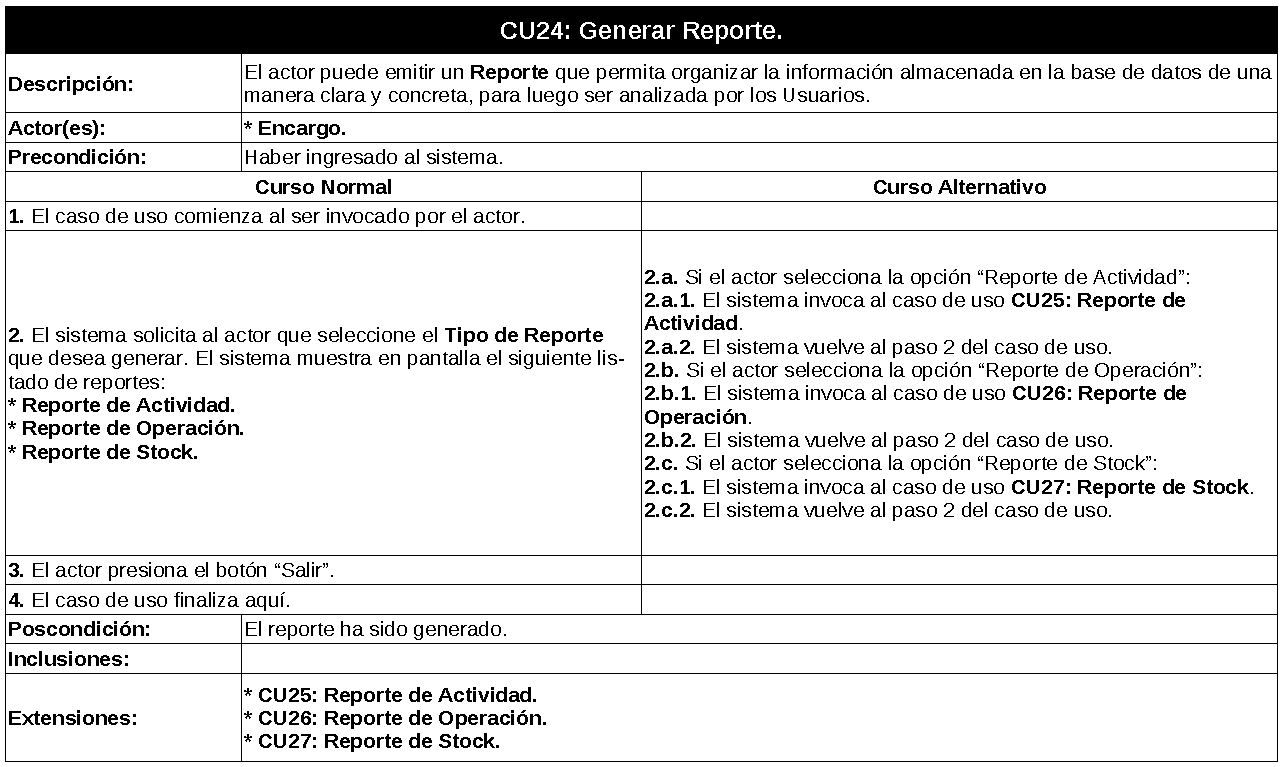
\includegraphics[scale=0.6]{Fichas_CU/pg_0024.pdf}}
\caption{CU24: Generar Reporte.}
\label{Ap224}
\end{figure}

\begin{figure}[tbhp]
\centerline{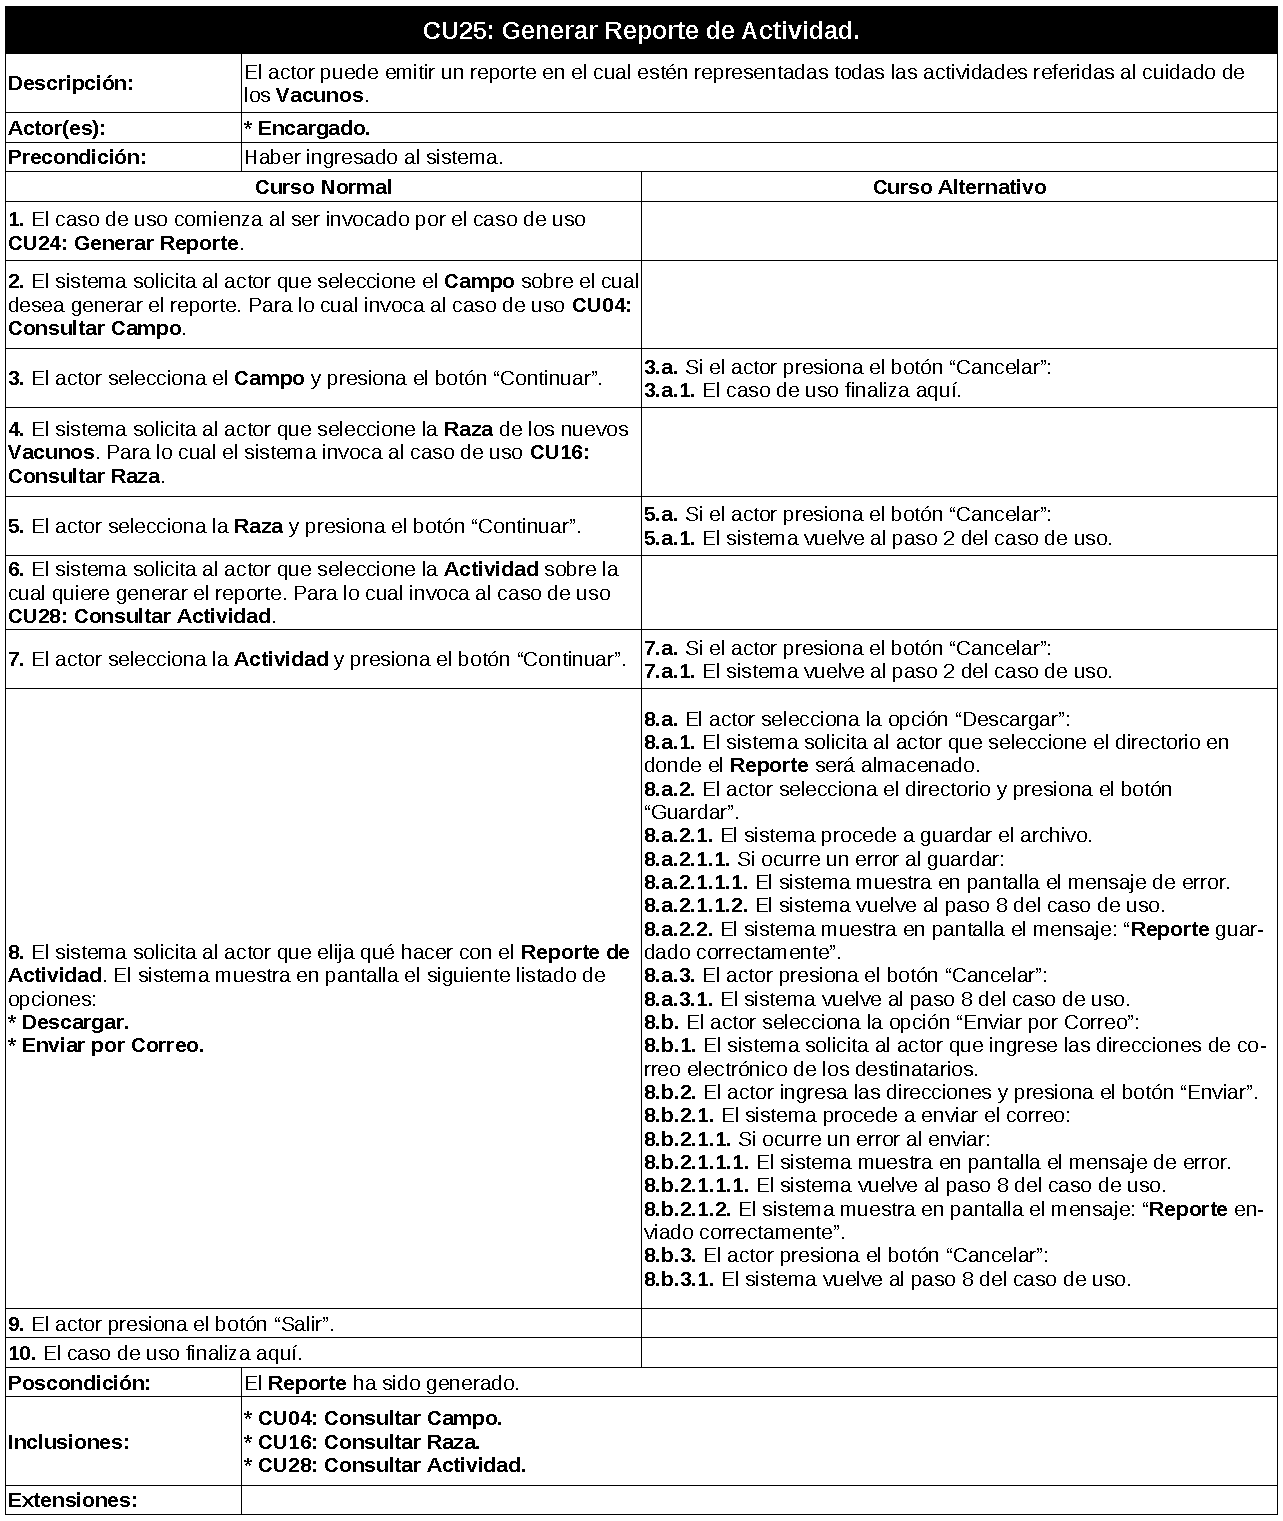
\includegraphics[scale=0.6]{Fichas_CU/pg_0025.pdf}}
\caption{CU25: Reporte de Actividad.}
\label{Ap225}
\end{figure}

\begin{figure}[tbhp]
\centerline{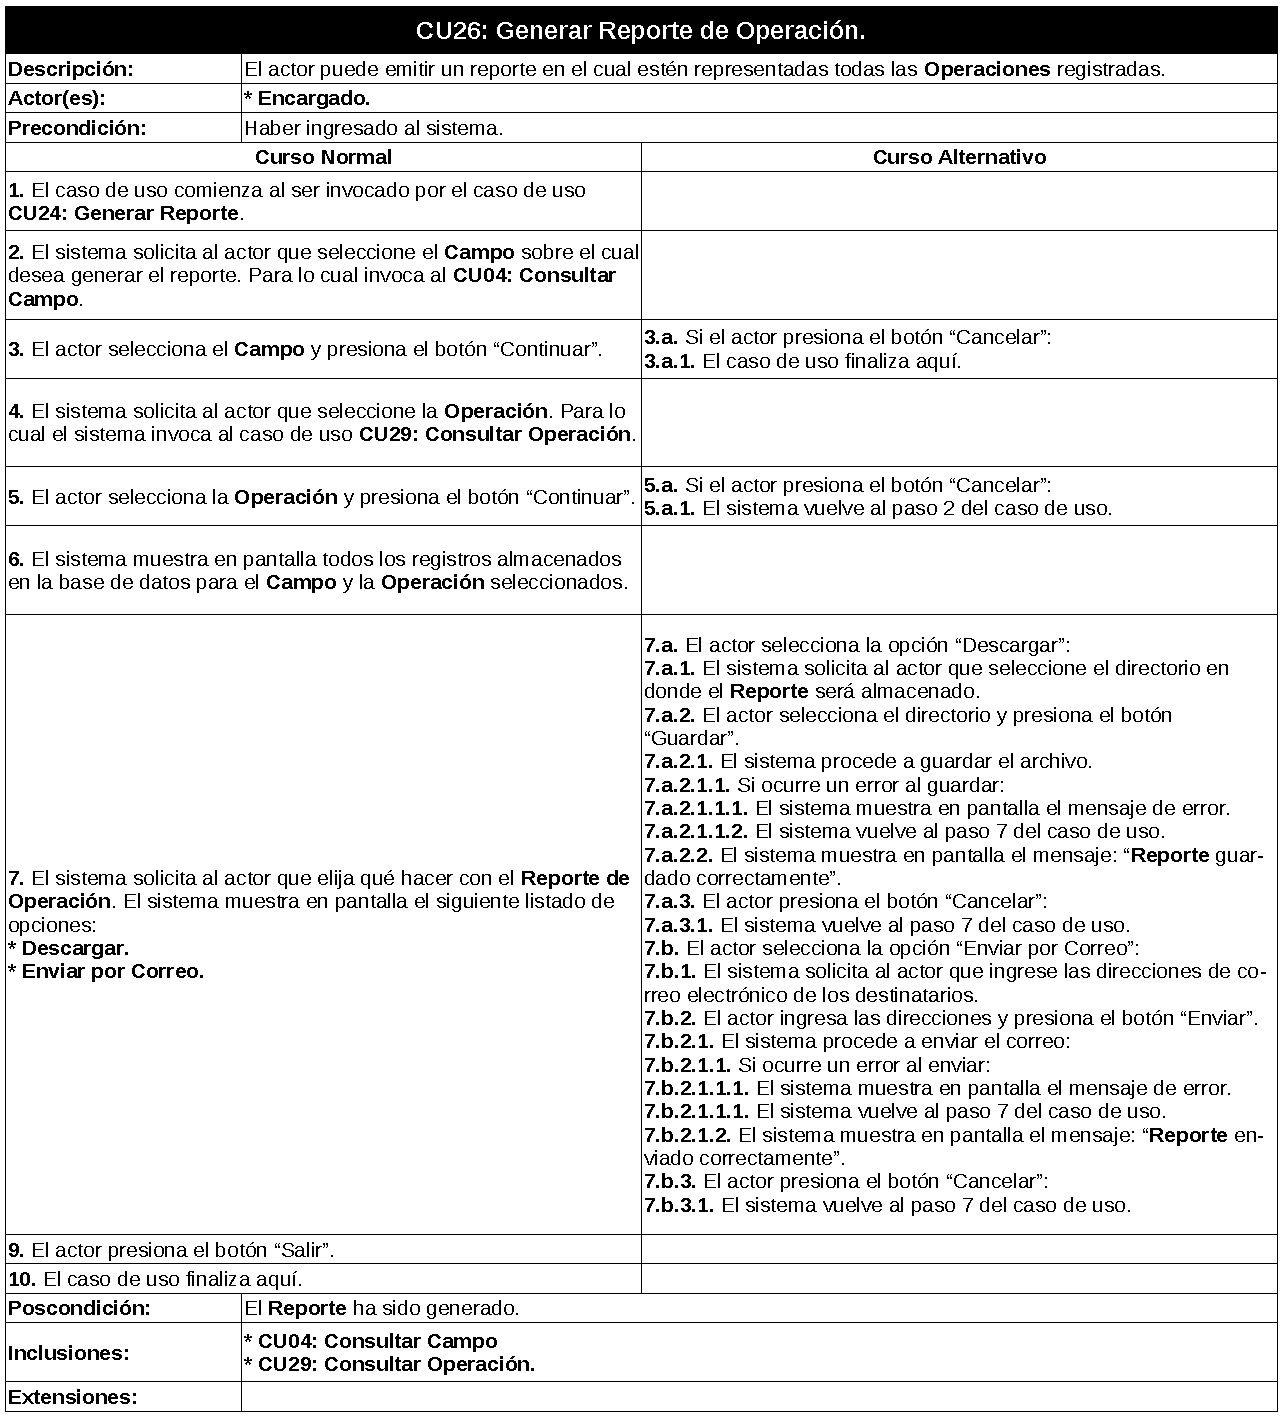
\includegraphics[scale=0.6]{Fichas_CU/pg_0026.pdf}}
\caption{CU26: Reporte de Operación.}
\label{Ap226}
\end{figure}

\begin{figure}[tbhp]
\centerline{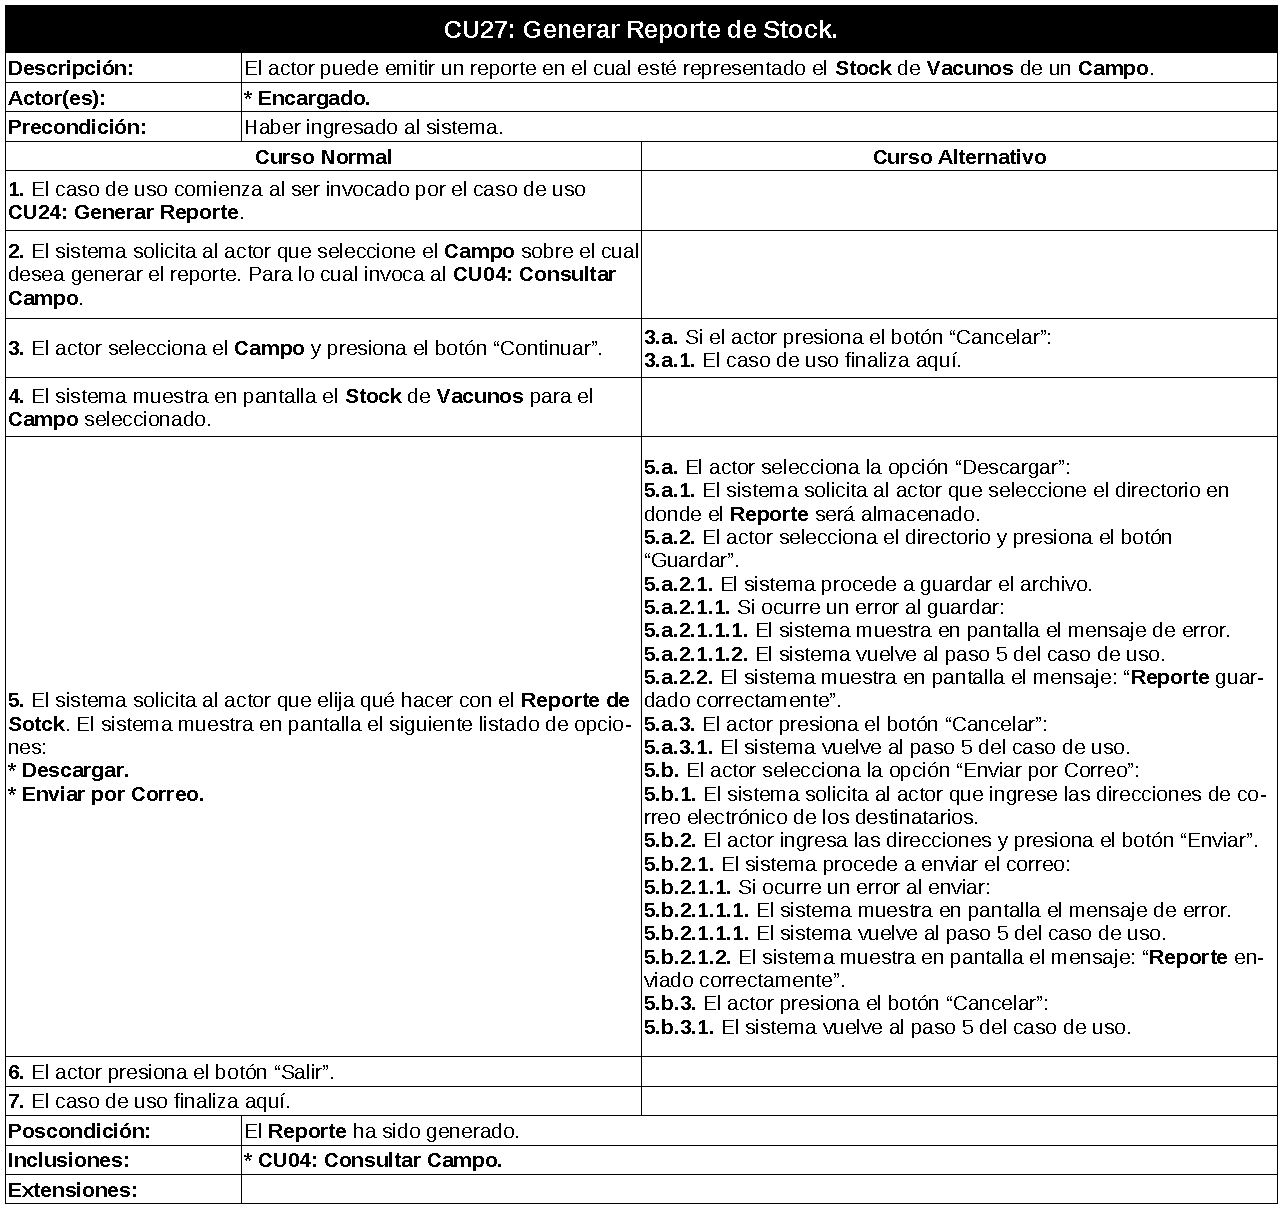
\includegraphics[scale=0.6]{Fichas_CU/pg_0027.pdf}}
\caption{CU27: Reporte de Stock.}
\label{Ap227}
\end{figure}

\begin{figure}[tbhp]
\centerline{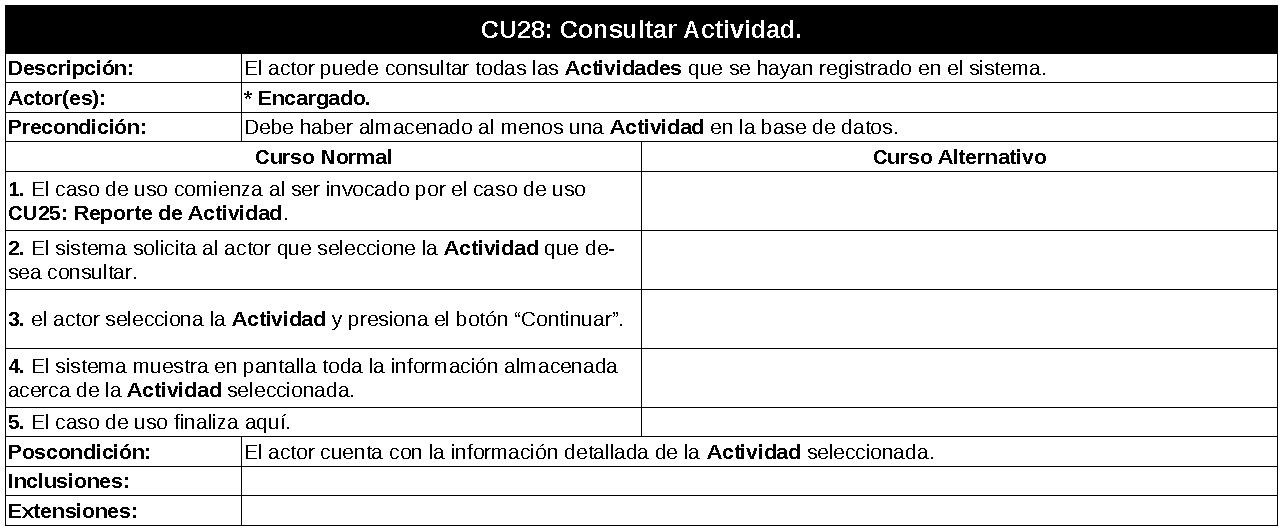
\includegraphics[scale=0.6]{Fichas_CU/pg_0028.pdf}}
\caption{CU28: Consultar Actividad.}
\label{Ap228}
\end{figure}

\begin{figure}[tbhp]
\centerline{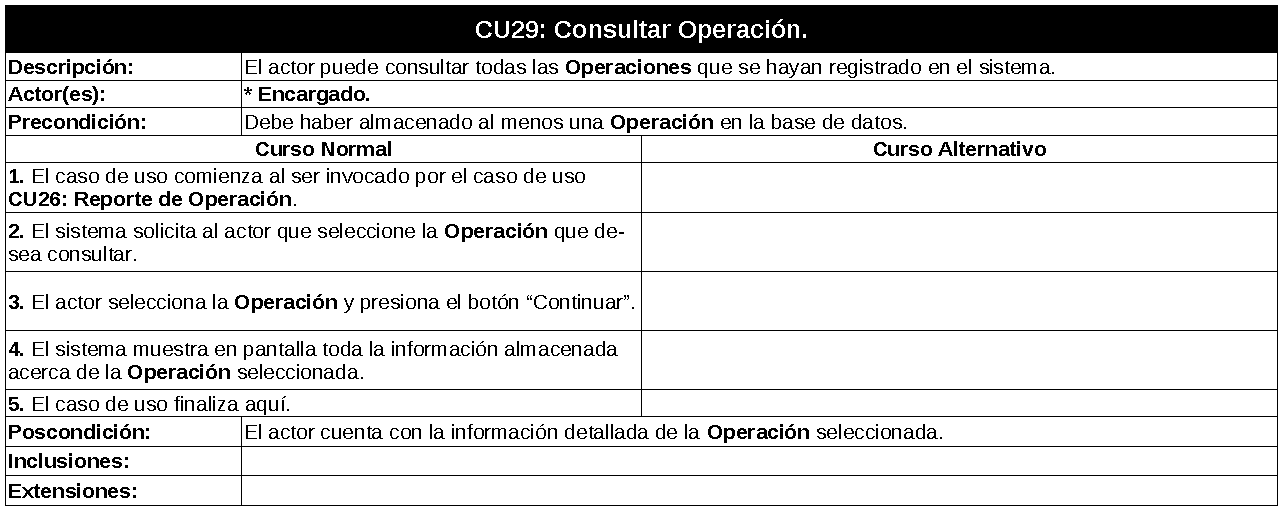
\includegraphics[scale=0.6]{Fichas_CU/pg_0029.pdf}}
\caption{CU29: Consultar Operación.}
\label{Ap229}
\end{figure}

\begin{figure}[tbhp]
\centerline{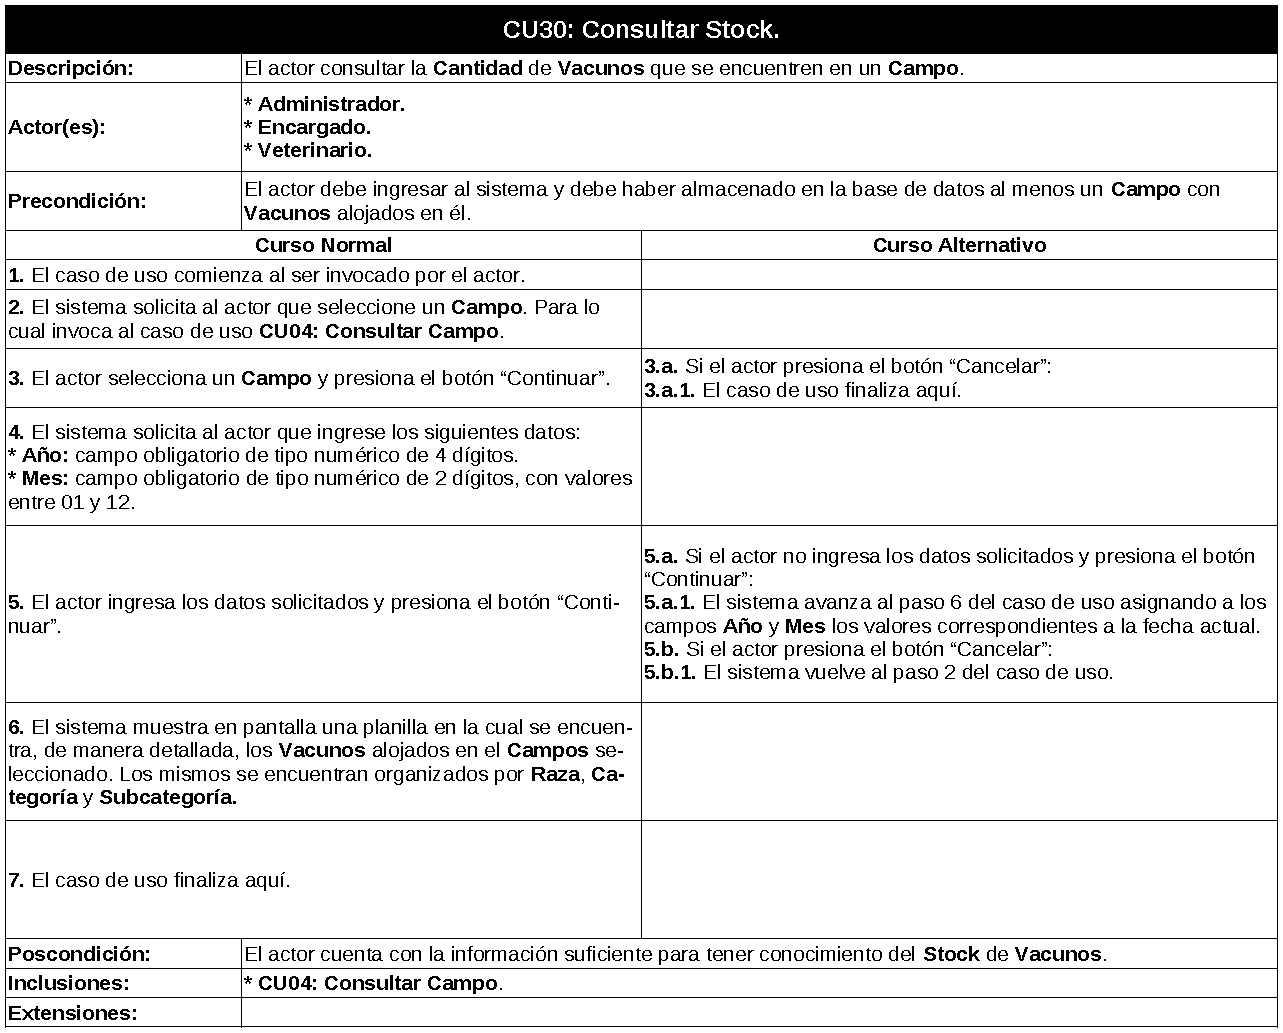
\includegraphics[scale=0.6]{Fichas_CU/pg_0030.pdf}}
\caption{CU30: Consultar Stock.}
\label{Ap230}
\end{figure}

\begin{figure}[tbhp]
\centerline{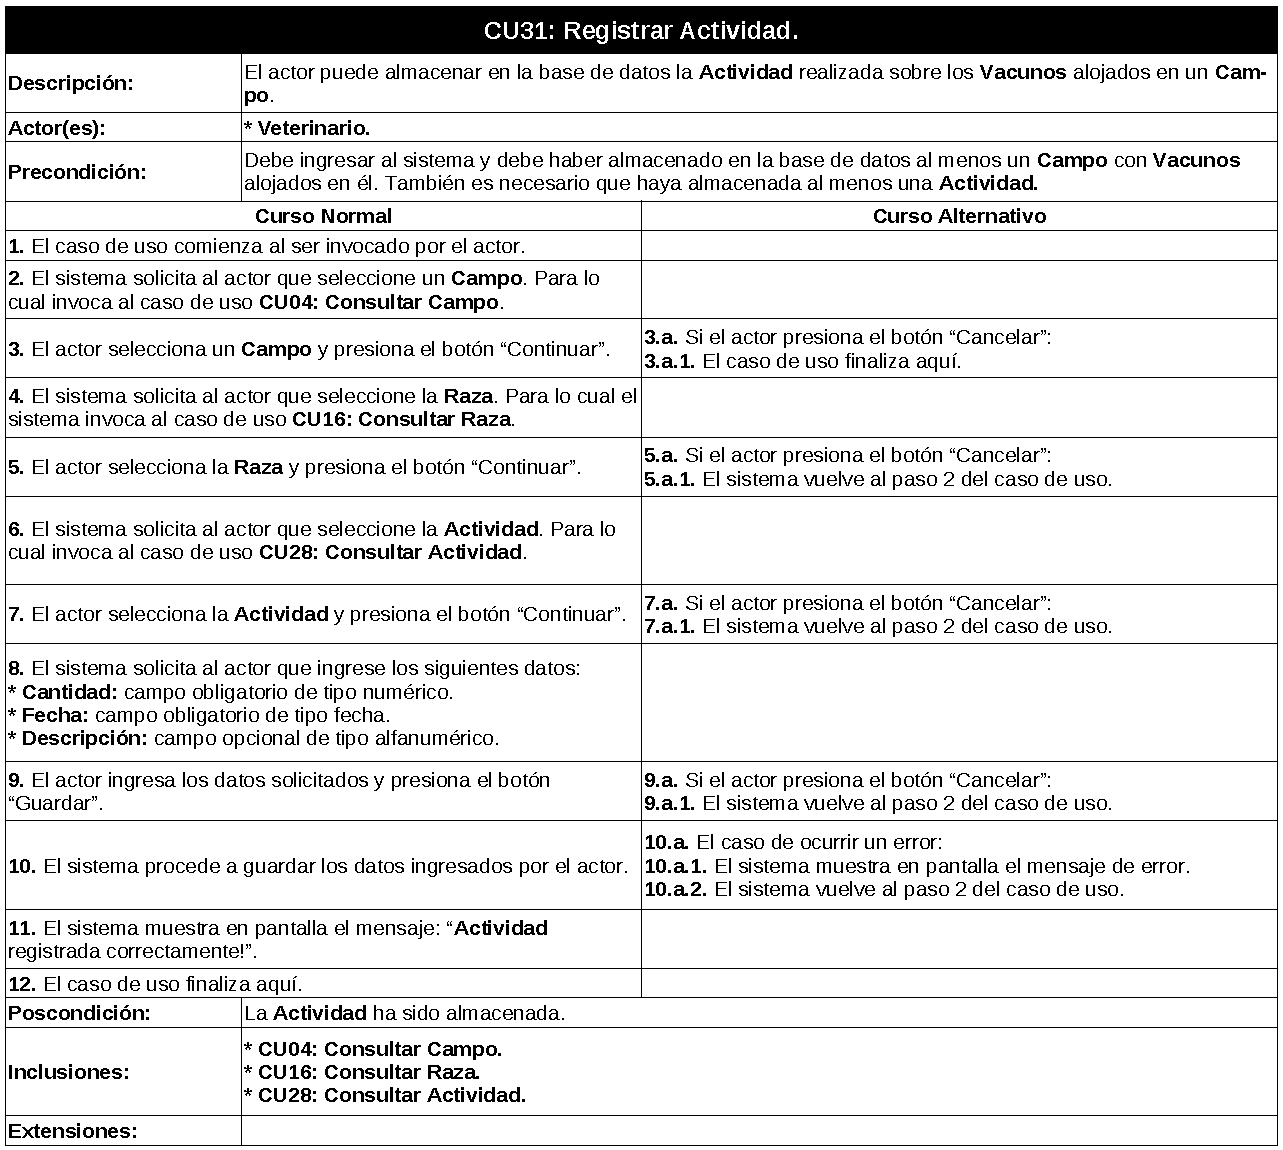
\includegraphics[scale=0.6]{Fichas_CU/pg_0031.pdf}}
\caption{CU31: Registrar Actividad.}
\label{Ap231}
\end{figure}

\begin{figure}[tbhp]
\centerline{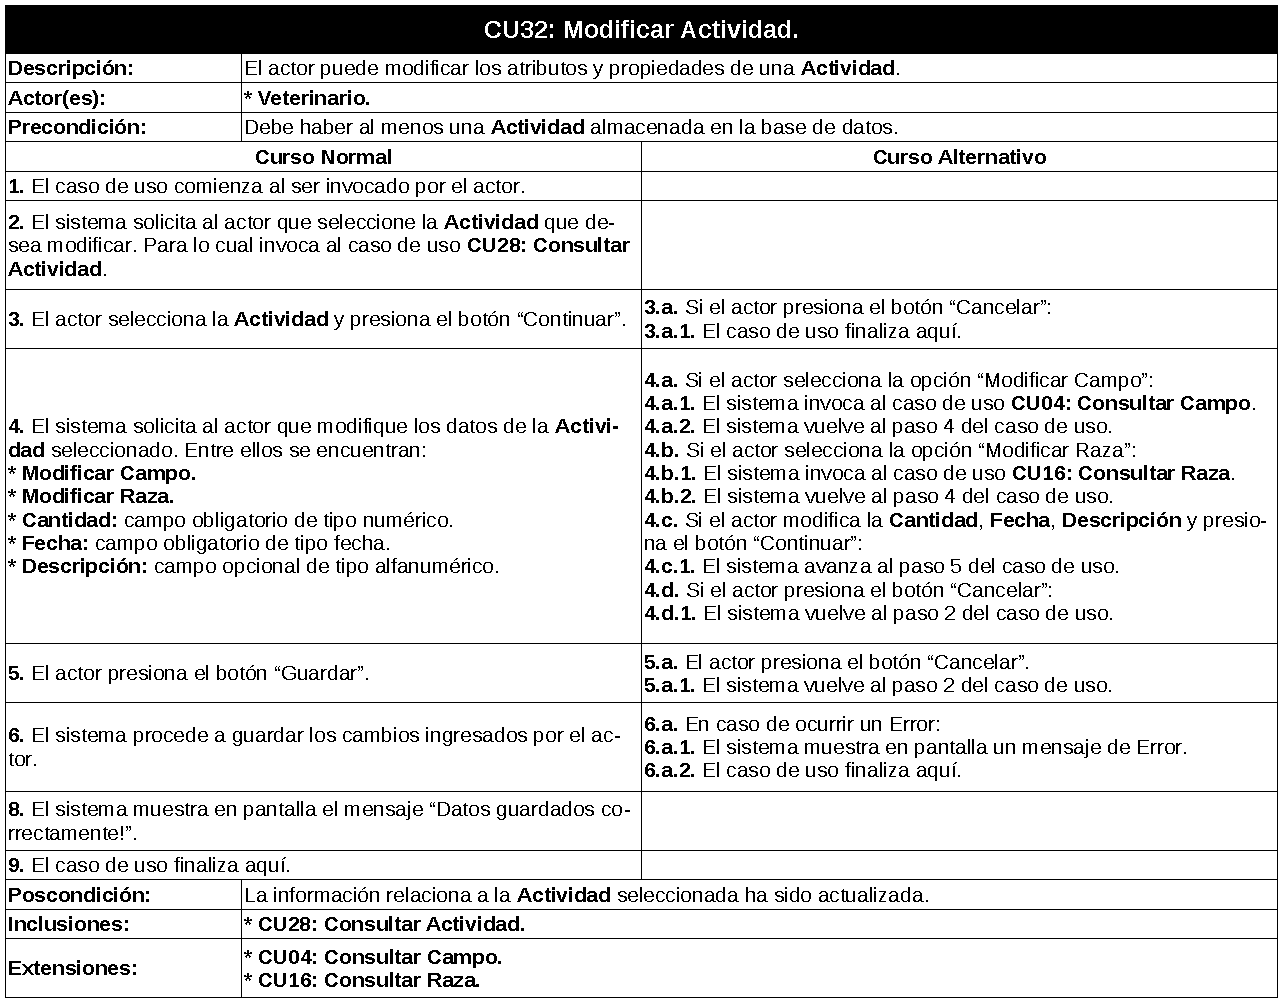
\includegraphics[scale=0.6]{Fichas_CU/pg_0032.pdf}}
\caption{CU32: Modificar Actividad.}
\label{Ap232}
\end{figure}

\begin{figure}[tbhp]
\centerline{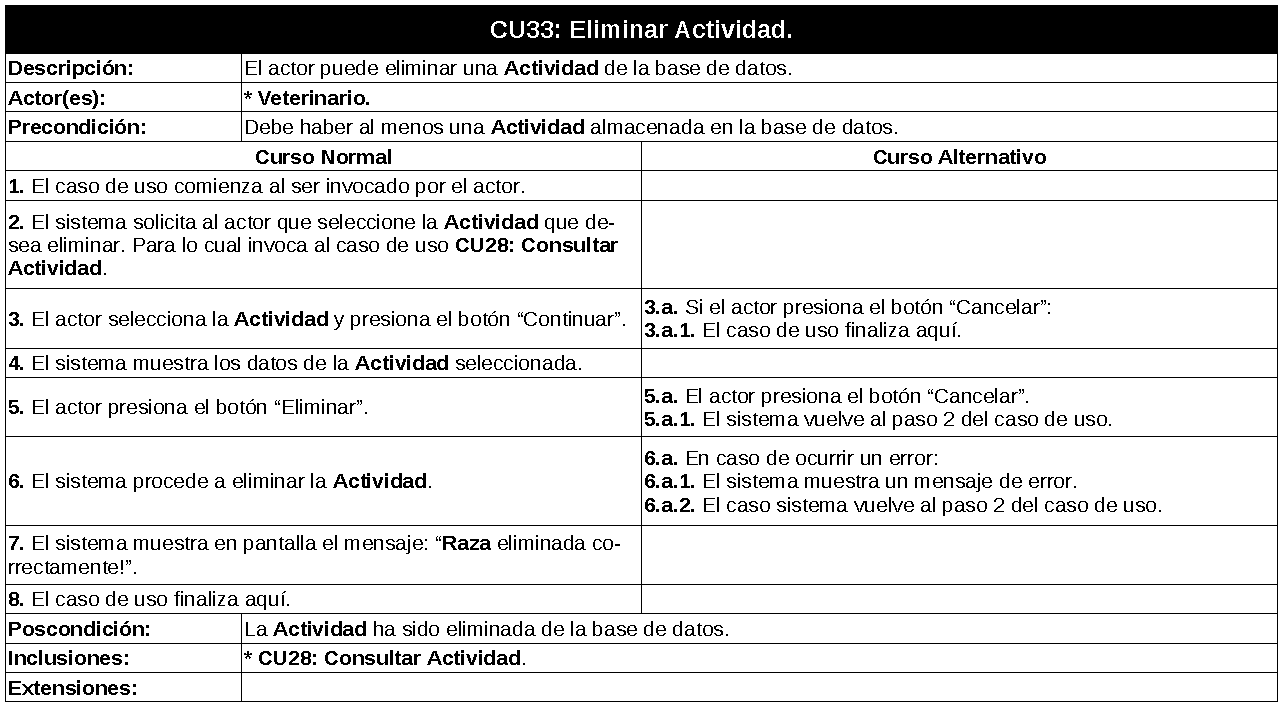
\includegraphics[scale=0.6]{Fichas_CU/pg_0033.pdf}}
\caption{CU33: Eliminar Actividad.}
\label{Ap233}
\end{figure}

\begin{figure}[tbhp]
\centerline{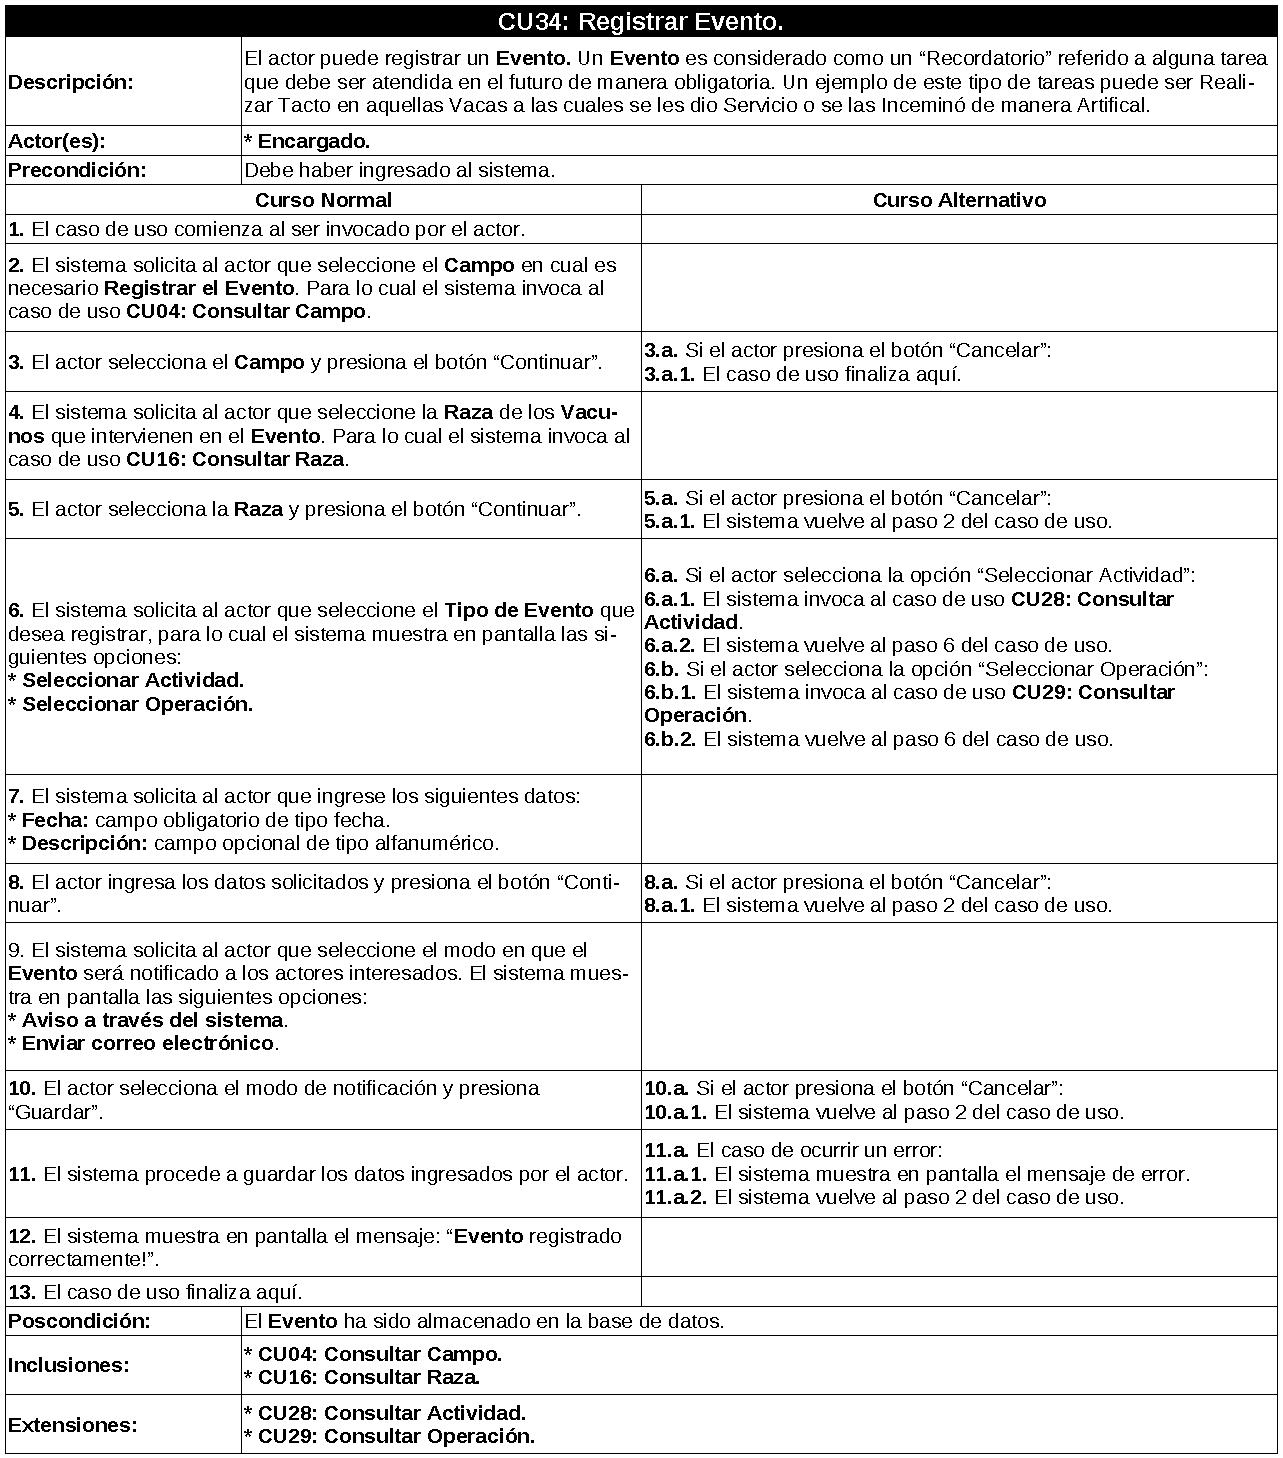
\includegraphics[scale=0.6]{Fichas_CU/pg_0034.pdf}}
\caption{CU34: Registrar Evento.}
\label{Ap234}
\end{figure}

\begin{figure}[tbhp]
\centerline{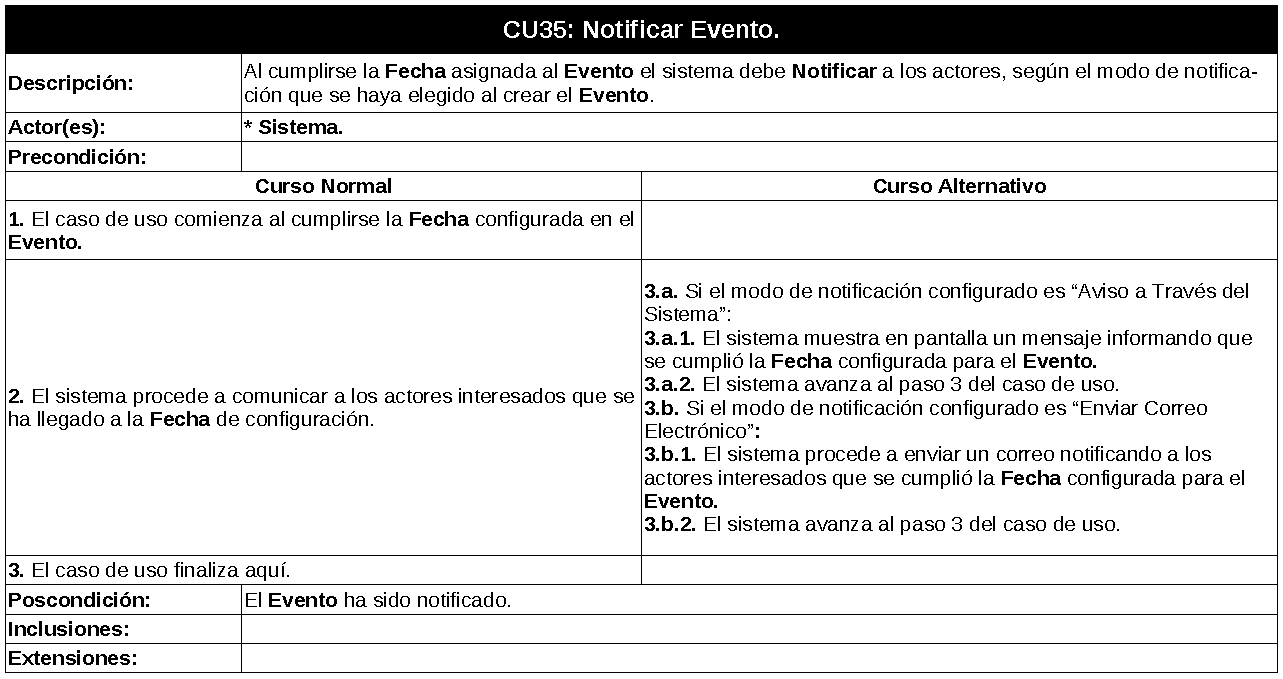
\includegraphics[scale=0.6]{Fichas_CU/pg_0035.pdf}}
\caption{CU35: Notificar Evento.}
\label{Ap235}
\end{figure}

\begin{figure}[tbhp]
\centerline{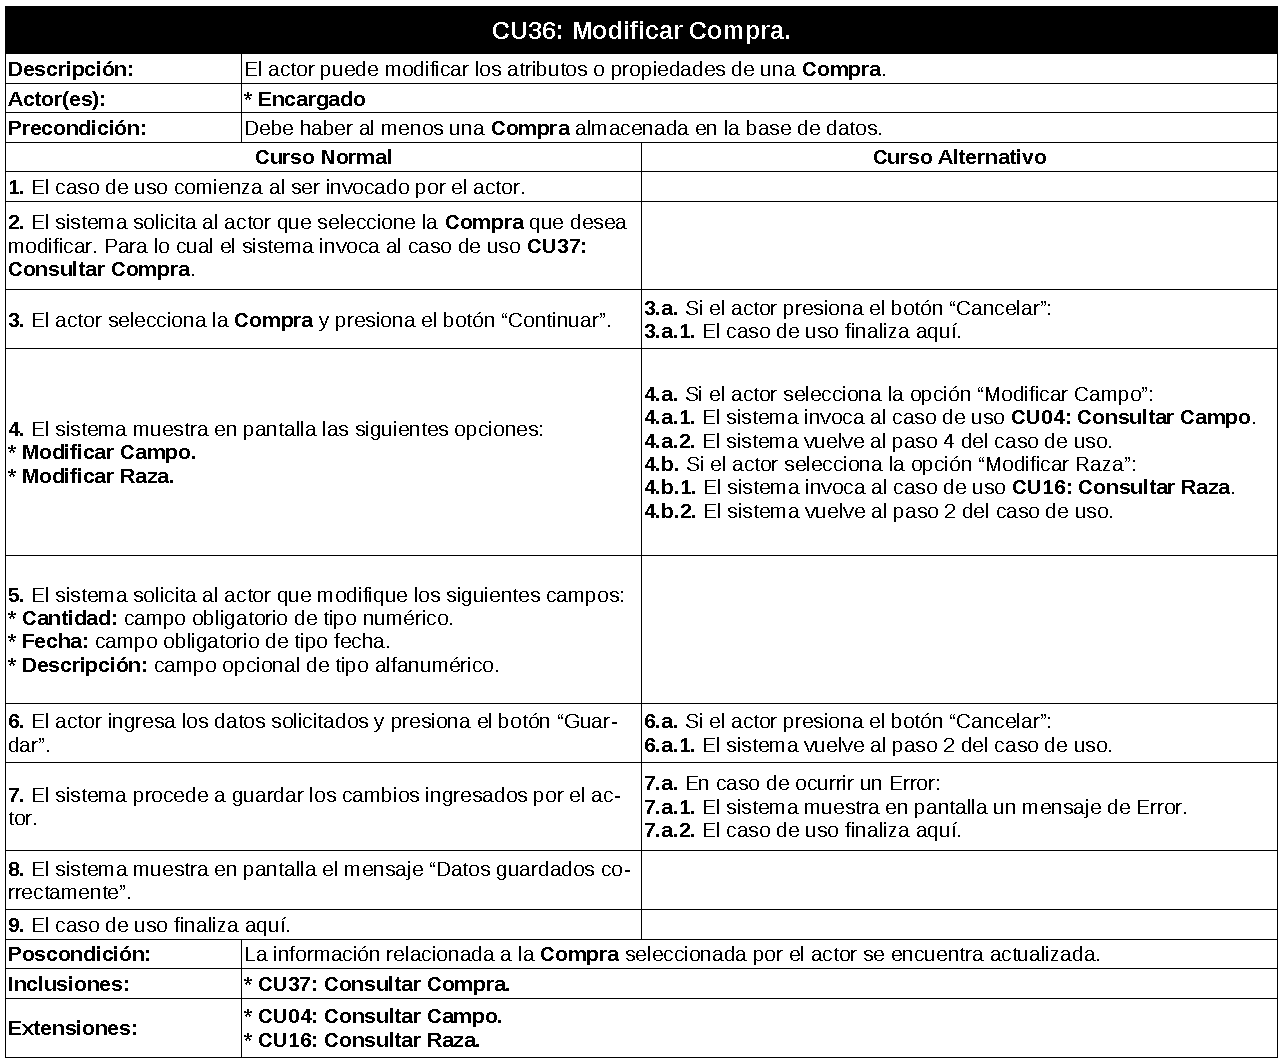
\includegraphics[scale=0.6]{Fichas_CU/pg_0036.pdf}}
\caption{CU36: Modificar Compra.}
\label{Ap236}
\end{figure}

\begin{figure}[tbhp]
\centerline{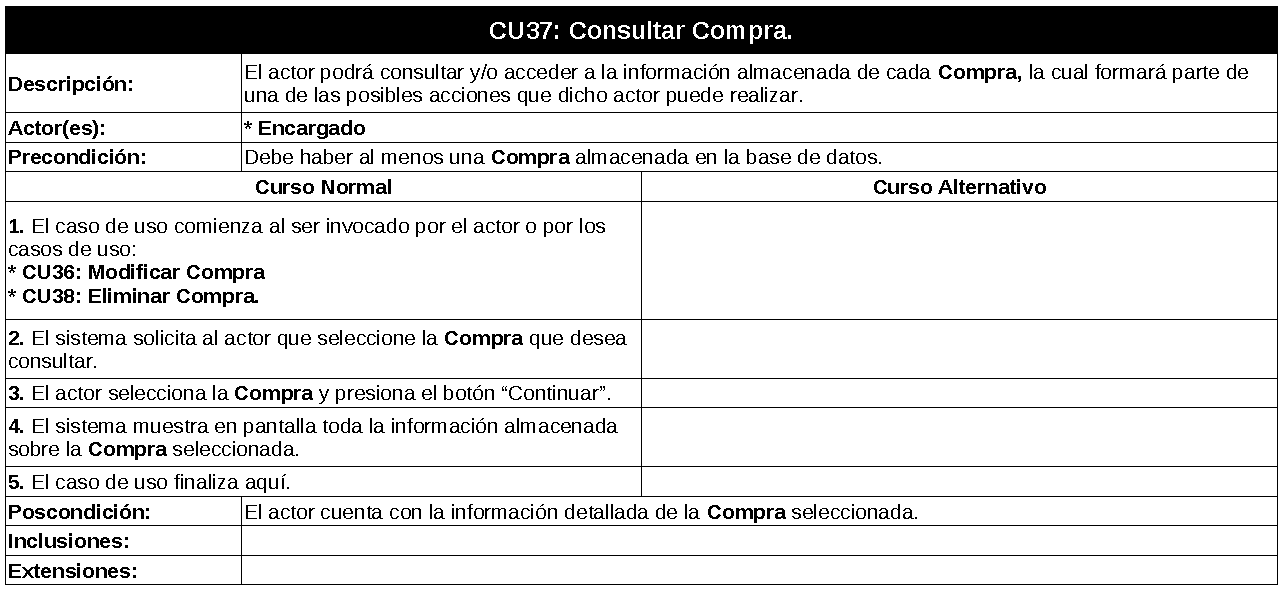
\includegraphics[scale=0.6]{Fichas_CU/pg_0037.pdf}}
\caption{CU37: Consultar Compra.}
\label{Ap237}
\end{figure}

\begin{figure}[tbhp]
\centerline{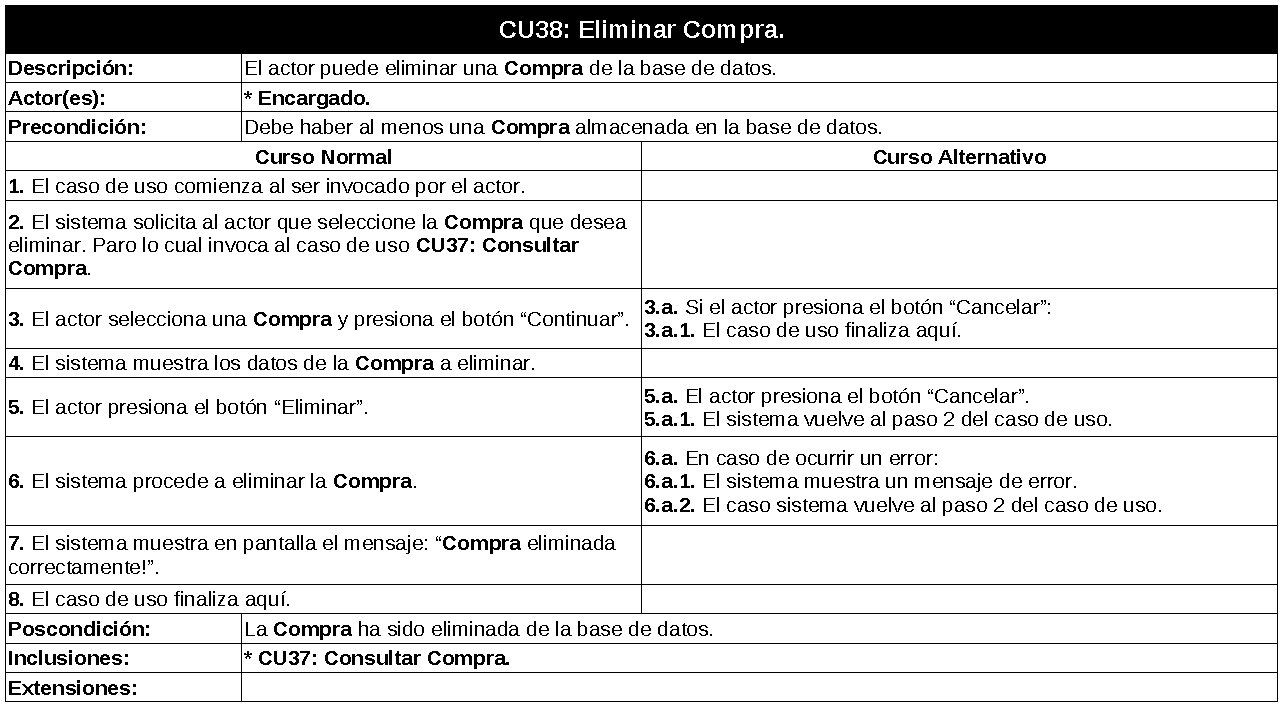
\includegraphics[scale=0.6]{Fichas_CU/pg_0038.pdf}}
\caption{CU38: Eliminar Compra.}
\label{Ap238}
\end{figure}

\begin{figure}[tbhp]
\centerline{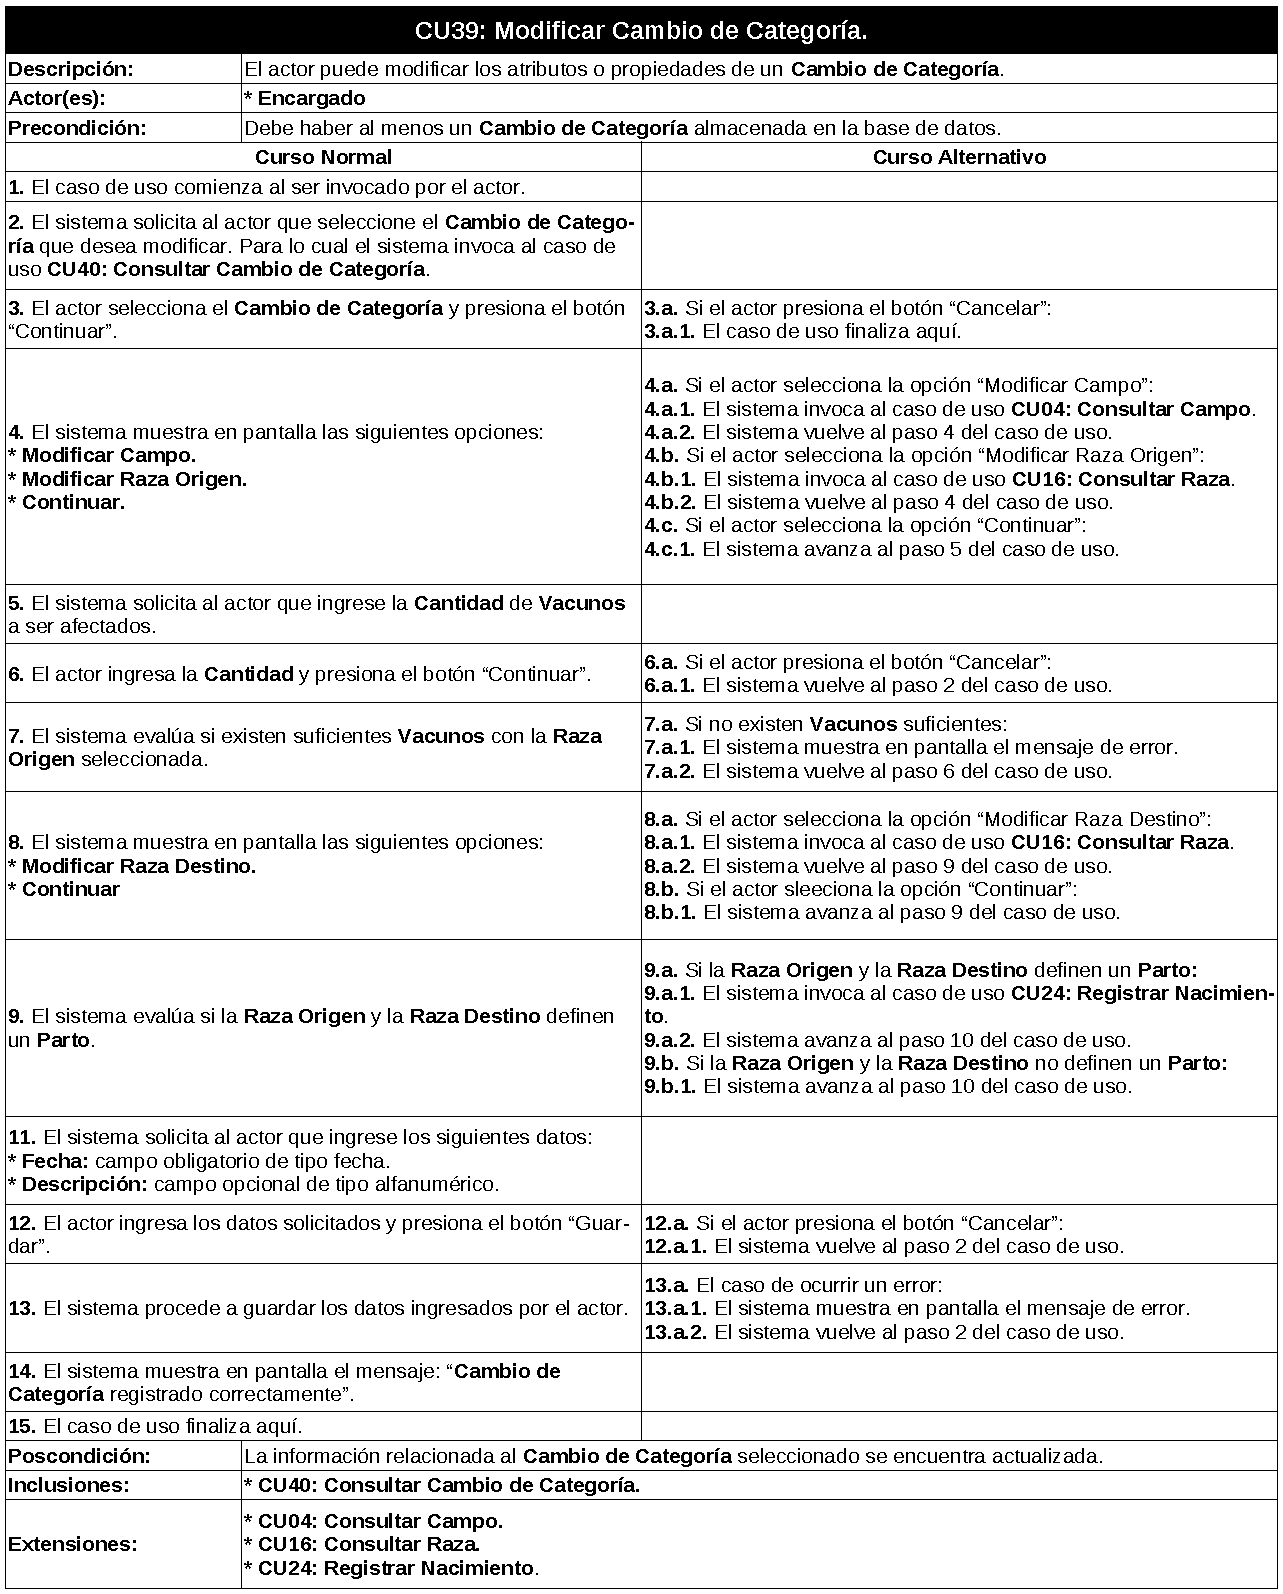
\includegraphics[scale=0.6]{Fichas_CU/pg_0039.pdf}}
\caption{CU39: Modificar Cambio de Categoria.}
\label{Ap239}
\end{figure}

\begin{figure}[tbhp]
\centerline{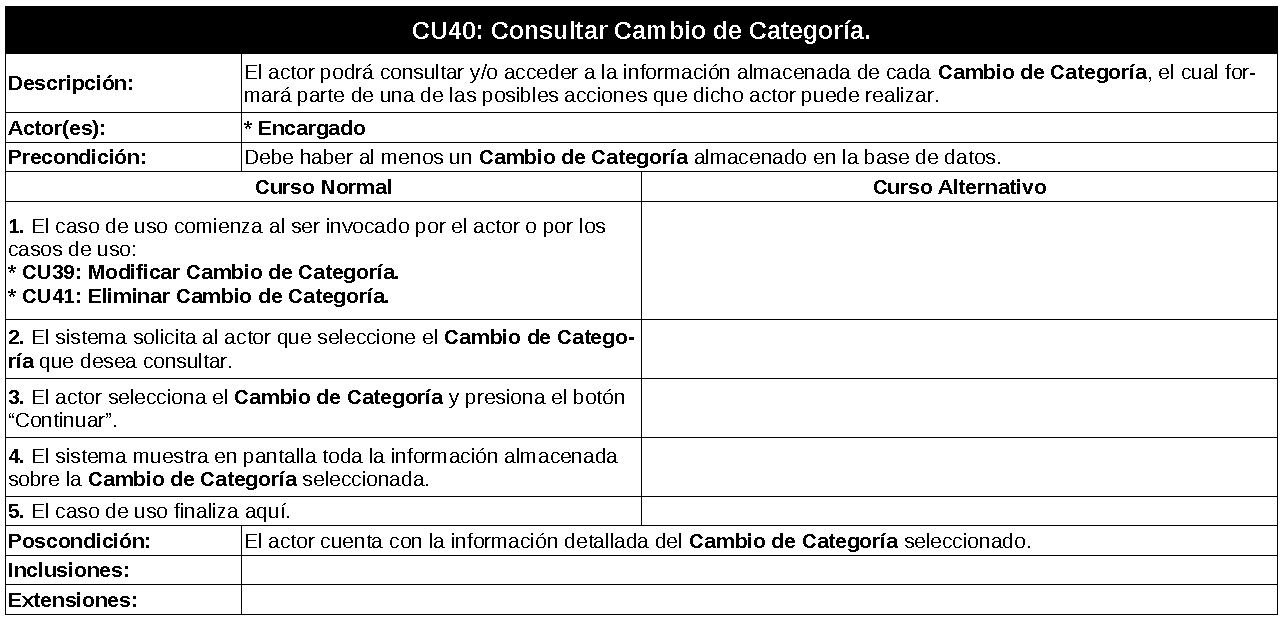
\includegraphics[scale=0.6]{Fichas_CU/pg_0040.pdf}}
\caption{CU40: Consultar Cambio de Categoria.}
\label{Ap240}
\end{figure}

\begin{figure}[tbhp]
\centerline{\includegraphics[scale=0.6]{Fichas_CU/pg_0041.pdf}}
\caption{CU41: Eliminar Cambio de Categoria.}
\label{Ap241}
\end{figure}

\begin{figure}[tbhp]
\centerline{\includegraphics[scale=0.6]{Fichas_CU/pg_0042.pdf}}
\caption{CU42: Modificar Traslado.}
\label{Ap242}
\end{figure}

\begin{figure}[tbhp]
\centerline{\includegraphics[scale=0.6]{Fichas_CU/pg_0043.pdf}}
\caption{CU43: Consultar Traslado.}
\label{Ap243}
\end{figure}

\begin{figure}[tbhp]
\centerline{\includegraphics[scale=0.6]{Fichas_CU/pg_0044.pdf}}
\caption{CU44: Eliminar Traslado.}
\label{Ap244}
\end{figure}

\begin{figure}[tbhp]
\centerline{\includegraphics[scale=0.6]{Fichas_CU/pg_0045.pdf}}
\caption{CU45: Modificar Venta.}
\label{Ap245}
\end{figure}

\begin{figure}[tbhp]
\centerline{\includegraphics[scale=0.6]{Fichas_CU/pg_0046.pdf}}
\caption{CU46: Consultar Venta.}
\label{Ap246}
\end{figure}

\begin{figure}[tbhp]
\centerline{\includegraphics[scale=0.6]{Fichas_CU/pg_0047.pdf}}
\caption{CU47: Eliminar Venta.}
\label{Ap247}
\end{figure}

\begin{figure}[tbhp]
\centerline{\includegraphics[scale=0.6]{Fichas_CU/pg_0048.pdf}}
\caption{CU48: Modificar Mortandad.}
\label{Ap248}
\end{figure}

\begin{figure}[tbhp]
\centerline{\includegraphics[scale=0.6]{Fichas_CU/pg_0049.pdf}}
\caption{CU49: Consultar Mortandad.}
\label{Ap249}
\end{figure}

\newpage
\clearpage
\begin{figure}[tbhp]
\centerline{\includegraphics[scale=0.6]{Fichas_CU/pg_0050.pdf}}
\caption{CU50: Eliminar Mortandad.}
\label{Ap250}
\end{figure}

\begin{figure}[tbhp]
\centerline{\includegraphics[scale=0.6]{Fichas_CU/pg_0051.pdf}}
\caption{CU51: Modificar Nacimiento.}
\label{Ap251}
\end{figure}

\begin{figure}[tbhp]
\centerline{\includegraphics[scale=0.6]{Fichas_CU/pg_0052.pdf}}
\caption{CU52: Consultar Nacimiento.}
\label{Ap252}
\end{figure}

\begin{figure}[tbhp]
\centerline{\includegraphics[scale=0.6]{Fichas_CU/pg_0053.pdf}}
\caption{CU53: Eliminar Nacimiento.}
\label{Ap253}
\end{figure}

\begin{figure}[tbhp]
\centerline{\includegraphics[scale=0.6]{Fichas_CU/pg_0054.pdf}}
\caption{CU54: Registrar Aborto.}
\label{Ap254}
\end{figure}

\begin{figure}[tbhp]
\centerline{\includegraphics[scale=0.6]{Fichas_CU/pg_0055.pdf}}
\caption{CU55: Modificar Aborto.}
\label{Ap255}
\end{figure}

\begin{figure}[tbhp]
\centerline{\includegraphics[scale=0.6]{Fichas_CU/pg_0056.pdf}}
\caption{CU56: Consultar Aborto.}
\label{Ap256}
\end{figure}

\begin{figure}[tbhp]
\centerline{\includegraphics[scale=0.6]{Fichas_CU/pg_0057.pdf}}
\caption{CU57: Eliminar Aborto.}
\label{Ap257}
\end{figure}

\begin{figure}[tbhp]
\centerline{\includegraphics[scale=0.6]{Fichas_CU/pg_0058.pdf}}
\caption{CU58: Registrar Destete.}
\label{Ap258}
\end{figure}

\begin{figure}[tbhp]
\centerline{\includegraphics[scale=0.6]{Fichas_CU/pg_0059.pdf}}
\caption{CU59: Modificar Destete.}
\label{Ap259}
\end{figure}

\begin{figure}[tbhp]
\centerline{\includegraphics[scale=0.6]{Fichas_CU/pg_0060.pdf}}
\caption{CU60: Consultar Destete.}
\label{Ap260}
\end{figure}

\begin{figure}[tbhp]
\centerline{\includegraphics[scale=0.6]{Fichas_CU/pg_0061.pdf}}
\caption{CU61: Eliminar Destete.}
\label{Ap261}
\end{figure}

%%%%%%%%%%%%%%%%%%%%%%%%%%%%%%%%%%%%%%%%%%%%% BIBLIOGRAFÍA %%%%%%%%%%%%%%%%%%%%%%%%%%%%%%%%%%%%%%%%%%%

%\renewcommand{\bibname}{\vspace{-2.5cm}\large{BIBLIOGRAFÍA}\vspace{-0.5cm}}
%\nocite{*}
%\bibliographystyle{documento}
%\fancypagestyle{plain}{%
%\fancyhf{}
%\fancyfoot[R]{\thepage}}
%\bibliography{documento}
%\addcontentsline{toc}{section}{\hspace{0.36cm}BIBLIOGRAFÍA}
\end{document}